% !TeX program = xelatex
% !TeX TXS-program:compile = txs:///xelatex/[--shell-escape]
%%%%%%%%%%%%%%%%%%%%%%%%%%%%%%%%%%%%%%%%%%%%%%%%%%%%%%%%%%%%%%%%%%%%%%%%
% Plantilla TFG/TFM
% Escuela Politécnica Superior de la Universidad de Alicante
% Realizado por: Jose Manuel Requena Plens
% Contacto: info@jmrplens.com / Telegram:@jmrplens
%%%%%%%%%%%%%%%%%%%%%%%%%%%%%%%%%%%%%%%%%%%%%%%%%%%%%%%%%%%%%%%%%%%%%%%%

% Elige si deseas optimizar la ejecución del proyecto almacenando las figuras generadas con TikZ y PGF en una carpeta (archivos/figuras-procesadas).
% 1 - Si, 2 - No
\def\OptimizaTikZ{1}

% Archivo .TEX que incluye todas las configuraciones del documento y los paquetes. Añade todo aquello que necesites utilizar en el documento en este archivo.
% En él se encuentra la configuración de los márgenes, establecidos según las directrices de estilo de la EPS.
\input{include/configuracioninicial}

% Obligatorio colocar en el main en la version para Overleaf, no eliminar
\if\OptimizaTikZ 1
\tikzexternalize[prefix=archivos/figuras-procesadas/] % Ruta
\fi 

%%%%%%%%%%%%%%%%%%%%%%%%%%%%%%%%%%%%%%%%%%%%%%%%%%%%%%%%%%%%%%%%%%%%%%
% INFORMACIÓN DEL TFG
% Comentar lo que NO se desee añadir y sustituir con la información correcta.
%%%%%%%%%%%%%%%%%%%%%%%%%%%%%%%%%%%%%%%%%%%%%%%%%%%%%%%%%%%%%%%%%%%%%%
% Título y subtítulo
\newcommand{\titulo}{Análisis comparativo de modelos de aprendizaje automático para la estimación del crecimiento del PIB en la zona euro}
\newcommand{\subtitulo}{}
% Datos del autor
\newcommand{\miNombre}{César Mora Gómez (alumno)}
\newcommand{\miEmail}{cmgm25@alu.ua.es}
% Datos del tutor/es
\newcommand{\miTutor}{Jorge Calvo Zaragoza (tutor1)}
\newcommand{\departamentoTutor}{Departamento de lenguajes y sistemas informáticos}
% Datos de la facultada y universidad
\newcommand{\miFacultad}{Escuela Politécnica Superior}
\newcommand{\miFacultadCorto}{EPS UA}
\newcommand{\miUniversidad}{\protect{Universidad de Alicante}}
\newcommand{\miUbicacion}{Alicante}

%%%%%%%%%%%%%%%%%%%%%%%%%%%%%%%%%%%%%%%%%%%%%%%%%%%%%%%%%%%%%%%%%%%%%%
% INDICA TU TITULACIÓN
% ID	GRADO -------------------------------------------------
% 1		Ingeniería en Imagen y Sonido en Telecomunicación
% 2		Ingeniería Civil
% 3		Ingeniería Química
% 4		Ingeniería Informática
% 5		Ingeniería Multimedia
% 6		Arquitectura Técnica
% 7		Arquitectura
% 8		Robótica
% %		%%%%%%%%%%%%
% ID	MÁSTER ------------------------------------------------
% A		Telecomunicación
% B		Caminos, Canales y Puertos
% C		Gestión en la Edificación
% D		Desarrollo Web
% E		Materiales, Agua, Terreno
% F		Informática
% G 	Automática y Robótica
% H		Prevención de riesgos laborales
% I		Gestión Sostenible Agua
% J		Desarrollo Aplicaciones Móviles
% K		Ingeniería Química
% L		Ciberseguridad
%%%%%%%%%%%%%%%%%%%%%%%%%%%%%%%%%%%%%%%%%%%%%%%%%%%%%%%%%%%%%%%%%%%%%%%%%
%!!!!!!!!!!!!!!!!!!!!!!!!!!!!!!!!!!!!!!!!!!!!!!!!!!!!!!!!!!!!!!!!!!!!!%%%
																		%
\def\IDtitulo{4} % INTRODUCE LA ID DE TU TITULACIÓN						%
																		%
%!!!!!!!!!!!!!!!!!!!!!!!!!!!!!!!!!!!!!!!!!!!!!!!!!!!!!!!!!!!!!!!!!!!!!%%%
%%%%%%%%%%%%%%%%%%%%%%%%%%%%%%%%%%%%%%%%%%%%%%%%%%%%%%%%%%%%%%%%%%%%%%%%%

% Configuración automática según el identificador elegido
\input{include/configuraciontitulacion} 

% Información añadida a las propiedades del archivo PDF.
\hypersetup{
pdfauthor = {\miNombre~(\miEmail)},
pdftitle = {\titulo},
}

%%%%%%%%%%%%%%%%%%%%%%%% 
% INICIO DEL DOCUMENTO
% A partir de aquí debes empezar a realizar tu TFG/TFM
%%%%%%%%%%%%%%%%%%%%%%%%
\begin{document}

% Números romanos hasta el mainmatter.
\frontmatter

% PORTADA
\input{include/portada/portada_color} % Portada Color
\input{include/portada/portada_bn} % Portada B/N

%%%%% PREAMBULO
% Incluye el .tex que contiene el preámbulo, agradecimientos y dedicatorias.
% \input{capitulos/preliminaresconagradecimientos} 

% Incluye después del archivo anterior el indice y lista de figuras, tablas y códigos.
\tableofcontents	% Índice
\listoffigures		% Índice de figuras
\listoftables		% Índice de tablas

% Inicia la numeración habitual.
\mainmatter

%%%%
% CONTENIDO. CAPÍTULOS DEL TRABAJO - Añade o elimina según tus necesidades
%%%%
%%%%%%%%%%%%%%%%%%%%%%%%%%%%%%%%%%%%%%%%%%%%%%%%%%%%%%%%%%%%%%%%%%%%%%%%
% Plantilla TFG/TFM
% Escuela Politécnica Superior de la Universidad de Alicante
% Realizado por: Jose Manuel Requena Plens
% Contacto: info@jmrplens.com / Telegram:@jmrplens
%%%%%%%%%%%%%%%%%%%%%%%%%%%%%%%%%%%%%%%%%%%%%%%%%%%%%%%%%%%%%%%%%%%%%%%%

\chapter{Introducción}

\section{Importancia del PIB}

El Producto Interior Bruto (PIB) es uno de los principales indicadores macroeconómicos utilizados para medir el nivel de actividad económica de un país. Este indicador recoge el valor monetario total de los bienes y servicios finales producidos dentro de una economía durante un periodo de tiempo determinado, generalmente un trimestre o un año. Debido a su carácter agregado, el PIB se ha consolidado como una referencia fundamental para analizar el desempeño económico de los países y evaluar la evolución de su actividad productiva.

Su evolución proporciona información clave sobre el crecimiento económico, los ciclos económicos y la salud general de una economía. A través del análisis de las variaciones del PIB es posible identificar periodos de expansión, desaceleración o recesión económica, así como evaluar el impacto de distintos factores económicos y políticos sobre el conjunto del sistema productivo.

La capacidad de anticipar cambios en el PIB resulta especialmente relevante para gobiernos, bancos centrales y agentes económicos, ya que permite una mejor planificación de políticas económicas y una toma de decisiones más informada. Por ejemplo, las autoridades monetarias utilizan las previsiones de crecimiento económico como una de las variables fundamentales para determinar la orientación de la política monetaria, mientras que los gobiernos emplean estas estimaciones para planificar políticas fiscales y presupuestarias.

Además de su uso como indicador del crecimiento económico, el PIB es una variable de referencia fundamental para instituciones nacionales e internacionales. Organismos como bancos centrales, gobiernos y entidades supranacionales utilizan la evolución del PIB para evaluar el ciclo económico, diseñar políticas económicas y comparar el desempeño de distintas economías.

En contextos como la Unión Europea, el análisis comparativo del PIB entre países resulta especialmente relevante, ya que permite identificar diferencias estructurales, procesos de convergencia económica y efectos derivados de políticas económicas comunes. Este tipo de análisis resulta esencial para comprender la evolución económica relativa de los distintos Estados miembros y para evaluar la efectividad de determinadas medidas económicas a nivel supranacional.

Por ello, disponer de herramientas que permitan analizar y anticipar la evolución del PIB adquiere una importancia estratégica tanto a nivel nacional como internacional. Una comprensión adecuada de las cuentas nacionales y de los indicadores asociados a la actividad económica resulta fundamental para el análisis macroeconómico moderno y para la correcta interpretación de la dinámica económica de los países. \citet{oecd_understanding_national_accounts_2014}

\section{Dificultad de la predicción económica}

La predicción de variables macroeconómicas presenta importantes desafíos debido a la naturaleza compleja y cambiante de los sistemas económicos. A diferencia de otros fenómenos en los que las relaciones entre variables pueden modelizarse mediante leyes relativamente estables, las economías están influenciadas por una gran variedad de factores institucionales, sociales y políticos que pueden modificar significativamente su comportamiento a lo largo del tiempo.

Factores internos y externos, como crisis financieras, cambios en la política económica o perturbaciones globales, pueden alterar de forma significativa la evolución del PIB. Eventos inesperados, como crisis económicas internacionales, conflictos geopolíticos o pandemias, pueden provocar cambios bruscos en la actividad económica que resultan difíciles de anticipar mediante modelos tradicionales.

A esta complejidad se suma el carácter no lineal de muchas relaciones económicas, así como la presencia de incertidumbre y eventos inesperados que dificultan la modelización precisa del comportamiento económico. Además, las economías presentan estructuras heterogéneas, con distintos niveles de desarrollo, especialización productiva y marcos institucionales, lo que complica la aplicación de modelos universales válidos para distintos países o periodos temporales.

Otro elemento relevante es la limitada disponibilidad de datos en tiempo real y las posibles revisiones posteriores de las estadísticas macroeconómicas. Las estimaciones iniciales del PIB y de otros indicadores económicos suelen revisarse a medida que se dispone de información más completa, lo que introduce un grado adicional de incertidumbre en los procesos de predicción económica.

En este contexto, la predicción del crecimiento económico se convierte en un problema especialmente complejo que combina incertidumbre estructural, limitaciones en la información disponible y posibles cambios en las relaciones entre variables económicas a lo largo del tiempo. \citet{stock_watson_2003}

Estas dificultades ponen de manifiesto la necesidad de explorar enfoques alternativos que permitan capturar patrones complejos en los datos y mejorar la capacidad predictiva frente a los métodos tradicionales.

\section{IA y reconocimiento de patrones en datos económicos}

En los últimos años, los avances en inteligencia artificial y aprendizaje automático han permitido desarrollar modelos capaces de identificar patrones complejos en grandes conjuntos de datos. Estas técnicas han demostrado su utilidad en numerosos ámbitos, como la visión artificial, el procesamiento del lenguaje natural o el análisis de grandes volúmenes de información, y su aplicación al análisis económico ha despertado un creciente interés tanto en el ámbito académico como en el profesional.

A diferencia de los enfoques econométricos clásicos, muchas técnicas de aprendizaje automático no requieren supuestos estrictos sobre la forma funcional de las relaciones entre variables. En lugar de definir previamente una estructura matemática concreta, estos modelos aprenden dichas relaciones directamente a partir de los datos disponibles, lo que les permite adaptarse a estructuras más complejas y dinámicas.

Su capacidad para analizar grandes volúmenes de datos y detectar patrones subyacentes las convierte en herramientas especialmente adecuadas para el estudio de fenómenos económicos, donde las relaciones entre variables pueden ser no lineales y estar sujetas a cambios a lo largo del tiempo. \citet{mullainathan_spiess_2017}

En este sentido, el uso de modelos basados en inteligencia artificial puede complementar los métodos tradicionales de análisis económico. Mientras que los enfoques econométricos clásicos se centran principalmente en la interpretación causal de las relaciones entre variables, muchas técnicas de aprendizaje automático priorizan la capacidad predictiva y la identificación de patrones en los datos.

Esta complementariedad ha motivado un creciente número de investigaciones que exploran la aplicación de técnicas de aprendizaje automático al análisis macroeconómico, incluyendo la predicción de variables agregadas como el crecimiento del PIB. \citet{pascual_ruiz_ml_series_2021}

\section{Objetivos}

A nivel personal, como estudiante del doble grado en Ingeniería Informática y Administración y Dirección de Empresas, este trabajo surge del interés por la aplicación de técnicas y modelos de inteligencia artificial al análisis económico. En particular, se pretende explorar cómo las economías responden ante distintos cambios a través del estudio de datos macroeconómicos, profundizando en el uso de técnicas de aprendizaje automático y en su capacidad para identificar patrones relevantes en este contexto.

El objetivo principal de este Trabajo de Fin de Grado es analizar y predecir la evolución del Producto Interior Bruto mediante técnicas de análisis de datos y aprendizaje automático, utilizando información macroeconómica de distintos países y evaluando el comportamiento de los modelos en diferentes escenarios.

Para ello, se plantea el desarrollo de un proceso completo que incluye la recopilación y preparación de datos macroeconómicos, la construcción de un conjunto de datos estructurado, el entrenamiento de modelos predictivos y la evaluación de su capacidad de generalización. Asimismo, se pretende analizar cómo la inclusión de distintas variables macroeconómicas puede influir en el rendimiento de los modelos de predicción.

Finalmente, como complemento al análisis realizado, se desarrolla una aplicación web interactiva que permite visualizar los resultados de los modelos, explorar las predicciones obtenidas y facilitar la interpretación de los experimentos realizados. Este componente busca aportar una dimensión más aplicada al trabajo, permitiendo representar de forma clara los resultados obtenidos durante el proceso de modelización.	% Plantilla: Se muestran contenidos
%%%%%%%%%%%%%%%%%%%%%%%%%%%%%%%%%%%%%%%%%%%%%%%%%%%%%%%%%%%%%%%%%%%%%%%%
% Plantilla TFG/TFM
% Escuela Politécnica Superior de la Universidad de Alicante
% Realizado por: Jose Manuel Requena Plens
% Contacto: info@jmrplens.com / Telegram:@jmrplens
%%%%%%%%%%%%%%%%%%%%%%%%%%%%%%%%%%%%%%%%%%%%%%%%%%%%%%%%%%%%%%%%%%%%%%%%

\chapter{Marco Teórico}
\label{marcoteorico}

\section{Predicción económica y series temporales}

La predicción económica constituye una herramienta fundamental para el análisis y la toma de decisiones en ámbitos como la política económica, la planificación empresarial o la evaluación del ciclo económico. En este contexto, muchas de las variables de interés, como el Producto Interior Bruto (PIB), la inflación o el empleo, se observan de forma periódica y ordenada en el tiempo, dando lugar a lo que se conoce como series temporales económicas.

Una serie temporal se define como una secuencia de observaciones de una variable registradas a lo largo del tiempo, donde el orden temporal y la dependencia entre observaciones consecutivas desempeñan un papel clave. A diferencia de otros tipos de datos, en las series temporales el valor observado en un momento determinado suele depender de valores anteriores de la misma variable, lo que introduce una estructura de dependencia temporal que debe ser considerada en los procesos de análisis y predicción.

Las series temporales económicas suelen presentar características específicas como tendencias, estacionalidad y persistencia. La tendencia hace referencia a la evolución de largo plazo de una variable, reflejando cambios estructurales en la economía. La estacionalidad, por su parte, recoge patrones que se repiten de forma periódica dentro de un mismo año, como puede ocurrir con ciertos indicadores de consumo o producción. Finalmente, la persistencia o dependencia temporal refleja la influencia que los valores pasados de una variable pueden tener sobre sus valores futuros. Estas características condicionan los enfoques utilizados para el análisis y la predicción de las series económicas. \citep{hyndman_athanasopoulos_fpp3}

En el ámbito de la predicción macroeconómica, el objetivo principal consiste en estimar el valor futuro de una variable a partir de la información disponible en el pasado. Para ello, es habitual utilizar tanto la propia historia de la variable que se desea predecir como otras variables económicas relacionadas que puedan aportar información relevante sobre su evolución futura.

Sin embargo, la predicción económica presenta importantes dificultades. Las economías están sujetas a cambios estructurales, shocks externos y comportamientos complejos de los agentes económicos, lo que puede alterar las relaciones entre variables a lo largo del tiempo. Además, la disponibilidad de datos suele ser limitada en comparación con otros ámbitos de aplicación del análisis de datos, especialmente cuando se trabaja con variables agregadas de carácter macroeconómico.

En este escenario, la predicción económica se plantea como un problema complejo que requiere un equilibrio entre simplicidad, capacidad explicativa y precisión predictiva. Este hecho ha motivado el desarrollo y la comparación de distintos enfoques de predicción, desde modelos sencillos de referencia hasta técnicas más avanzadas, con el objetivo de mejorar la capacidad para anticipar la evolución futura de las principales variables macroeconómicas. \citep{green_armstrong_2015}

Tradicionalmente, la predicción de series temporales económicas se ha abordado mediante modelos estadísticos y econométricos que buscan capturar la estructura temporal de los datos. No obstante, en los últimos años han surgido nuevas aproximaciones basadas en técnicas de aprendizaje automático, que permiten modelizar relaciones más complejas entre variables y aprovechar mejor la información disponible en los datos.

Estas nuevas aproximaciones no sustituyen necesariamente a los métodos tradicionales, sino que en muchos casos actúan como herramientas complementarias. Mientras que los modelos econométricos clásicos suelen centrarse en la interpretación estructural de las relaciones económicas, los modelos de aprendizaje automático priorizan la capacidad predictiva y la detección de patrones en los datos, lo que puede resultar especialmente útil en problemas de predicción económica.

\section{Modelos de aprendizaje automático para predicción económica}

En los últimos años, el desarrollo de técnicas de aprendizaje automático ha abierto nuevas posibilidades para el análisis y la predicción de variables económicas. A diferencia de muchos modelos econométricos tradicionales, que requieren especificar previamente una relación funcional concreta entre variables, los modelos de aprendizaje automático permiten aprender estas relaciones directamente a partir de los datos.

Estas técnicas han demostrado un gran potencial en problemas donde las relaciones entre variables pueden ser complejas, no lineales o difíciles de especificar mediante modelos estadísticos tradicionales. En particular, los algoritmos de aprendizaje supervisado permiten construir modelos predictivos a partir de conjuntos de datos históricos, identificando patrones que pueden utilizarse posteriormente para estimar valores futuros.

En el ámbito de la predicción económica, estas técnicas resultan especialmente interesantes cuando se dispone de múltiples variables explicativas que pueden influir en la evolución de un indicador macroeconómico. Variables como el empleo, la inflación o indicadores de actividad económica pueden aportar información relevante para anticipar la evolución del PIB, aunque la relación exacta entre ellas no siempre sea sencilla de modelizar mediante enfoques tradicionales.

Entre los algoritmos de aprendizaje automático más utilizados en problemas de predicción con datos tabulares se encuentran métodos basados en árboles de decisión y técnicas de ensamblado de modelos (\textit{ensemble learning}). Estos enfoques combinan múltiples modelos simples con el objetivo de mejorar la precisión predictiva y reducir el riesgo de sobreajuste.

Dentro de esta familia de métodos, los algoritmos basados en \textit{boosting} han demostrado un rendimiento especialmente destacado en problemas de predicción con datos estructurados, lo que ha motivado su creciente utilización en distintos ámbitos del análisis de datos.

\section{Gradient Boosting}

El \textit{Gradient Boosting} es una técnica de aprendizaje automático basada en la combinación secuencial de múltiples modelos simples con el objetivo de construir un modelo predictivo más preciso. Este enfoque pertenece a la familia de métodos de ensamblado, cuyo principio fundamental consiste en combinar varios modelos individuales para obtener un rendimiento superior al que se obtendría utilizando un único modelo. \citep{friedman_gradient_boosting_2001, zhou_ensemble_2012}

En el caso del \textit{boosting}, los modelos se construyen de forma secuencial, de modo que cada nuevo modelo intenta corregir los errores cometidos por los modelos anteriores. Habitualmente, estos modelos base son árboles de decisión de baja profundidad, lo que permite capturar relaciones no lineales entre variables sin introducir una complejidad excesiva. \citep{friedman_gradient_boosting_2001}

\begin{figure}[H]
\centering
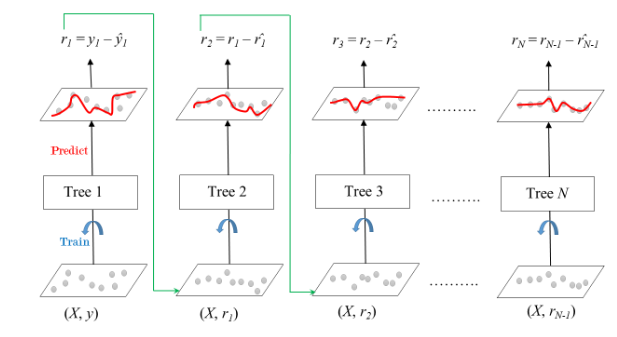
\includegraphics[width=0.9\textwidth]{figures/gradientboosting.png}
\caption{Proceso iterativo de entrenamiento en Gradient Boosting. Cada nuevo árbol se entrena para aproximar los errores residuales del modelo anterior, construyendo progresivamente una predicción más precisa.}
\label{fig:gradient_boosting}
\end{figure}

Como se observa en la figura \ref{fig:gradient_boosting}, el proceso de entrenamiento comienza con un modelo inicial relativamente simple que realiza una primera aproximación a la variable objetivo. A continuación, se calcula el error cometido por dicho modelo y se entrena un nuevo modelo que intenta explicar ese error. Este proceso se repite de forma iterativa, añadiendo nuevos modelos que van corrigiendo progresivamente los errores residuales de los modelos anteriores. \citep{friedman_gradient_boosting_2001}

El término \textit{gradient} hace referencia al uso del gradiente de la función de pérdida para determinar la dirección en la que debe ajustarse el modelo en cada iteración. En términos generales, el algoritmo busca minimizar una función de pérdida que mide la diferencia entre las predicciones del modelo y los valores reales observados. \citep{friedman_gradient_boosting_2001}

Este enfoque permite construir modelos muy flexibles capaces de capturar relaciones complejas entre variables, lo que explica su buen rendimiento en numerosos problemas de predicción. No obstante, también requiere un control cuidadoso de parámetros como la profundidad de los árboles o la tasa de aprendizaje para evitar problemas de sobreajuste.

\section{XGBoost}

XGBoost (\textit{Extreme Gradient Boosting}) es una implementación optimizada del algoritmo de \textit{Gradient Boosting} diseñada para mejorar la eficiencia computacional y el rendimiento predictivo. Este algoritmo ha ganado una gran popularidad en el ámbito del aprendizaje automático debido a su alto rendimiento en problemas de predicción con datos estructurados.

Una de las principales características de XGBoost es la incorporación de técnicas de regularización que permiten controlar la complejidad del modelo y reducir el riesgo de sobreajuste. A diferencia de implementaciones más básicas de \textit{boosting}, XGBoost incluye términos de penalización que limitan el crecimiento excesivo de los árboles de decisión y favorecen modelos más robustos. \citep{chen_guestrin_2016}

Además, XGBoost introduce diversas mejoras en términos de eficiencia computacional, como el uso de paralelización en el entrenamiento, optimizaciones en el manejo de memoria y técnicas avanzadas para el procesamiento de datos. Estas características permiten entrenar modelos de forma rápida incluso cuando se trabaja con conjuntos de datos relativamente grandes. \citep{chen_guestrin_2016}

En el contexto de la predicción económica, XGBoost resulta especialmente adecuado para trabajar con datos tabulares que incluyen múltiples variables explicativas. Su capacidad para capturar relaciones no lineales y efectos de interacción entre variables lo convierte en una herramienta potente para analizar la relación entre distintos indicadores macroeconómicos y la evolución del PIB. \citep{chen_guestrin_2016}

Por estas razones, XGBoost ha sido ampliamente utilizado en distintos ámbitos del análisis de datos y ha demostrado un alto rendimiento en competiciones de aprendizaje automático y aplicaciones reales. Su equilibrio entre capacidad predictiva, eficiencia computacional y control del sobreajuste lo convierte en una opción especialmente atractiva para problemas de predicción económica. La Figura~\ref{fig:decision_tree} muestra la estructura interna de un árbol de decisión individual de profundidad 3, el tipo de modelo base que emplea XGBoost.

\begin{figure}[H]
\centering
\resizebox{\linewidth}{!}{%
\begin{tikzpicture}[
  nodo/.style={draw, rounded corners=3pt, fill=blue!10, minimum width=1.8cm,
               minimum height=0.75cm, align=center, font=\small},
  hoja/.style={draw, rounded corners=3pt, fill=green!15, minimum width=1.2cm,
               minimum height=0.65cm, align=center, font=\small},
  arr/.style={->, >=stealth, thick},
  etiq/.style={font=\scriptsize, inner sep=2pt}
]

% --- Nivel 0 (raíz) ---
\node[nodo] (n0) {$x_1 < \theta_1$};

% --- Nivel 1 ---
\node[nodo, below left=1.0cm and 1.6cm of n0]  (n1l) {$x_2 < \theta_2$};
\node[nodo, below right=1.0cm and 1.6cm of n0] (n1r) {$x_3 < \theta_3$};

% --- Nivel 2 ---
\node[nodo, below left=0.9cm and 0.4cm of n1l]  (n2ll) {$x_4 < \theta_4$};
\node[nodo, below right=0.9cm and 0.4cm of n1l] (n2lr) {$x_5 < \theta_5$};
\node[nodo, below left=0.9cm and 0.4cm of n1r]  (n2rl) {$x_6 < \theta_6$};
\node[nodo, below right=0.9cm and 0.4cm of n1r] (n2rr) {$x_7 < \theta_7$};

% --- Nivel 3 (hojas) ---
\node[hoja, below left=0.8cm and 0.1cm of n2ll]  (h1) {$\hat{y}_1$};
\node[hoja, below right=0.8cm and 0.1cm of n2ll] (h2) {$\hat{y}_2$};
\node[hoja, below left=0.8cm and 0.1cm of n2lr]  (h3) {$\hat{y}_3$};
\node[hoja, below right=0.8cm and 0.1cm of n2lr] (h4) {$\hat{y}_4$};
\node[hoja, below left=0.8cm and 0.1cm of n2rl]  (h5) {$\hat{y}_5$};
\node[hoja, below right=0.8cm and 0.1cm of n2rl] (h6) {$\hat{y}_6$};
\node[hoja, below left=0.8cm and 0.1cm of n2rr]  (h7) {$\hat{y}_7$};
\node[hoja, below right=0.8cm and 0.1cm of n2rr] (h8) {$\hat{y}_8$};

% --- Flechas nivel 0 → 1 ---
\draw[arr] (n0.south) -- (n1l.north) node[etiq, midway, above left]{sí};
\draw[arr] (n0.south) -- (n1r.north) node[etiq, midway, above right]{no};

% --- Flechas nivel 1 → 2 ---
\draw[arr] (n1l.south) -- (n2ll.north) node[etiq, midway, above left]{sí};
\draw[arr] (n1l.south) -- (n2lr.north) node[etiq, midway, above right]{no};
\draw[arr] (n1r.south) -- (n2rl.north) node[etiq, midway, above left]{sí};
\draw[arr] (n1r.south) -- (n2rr.north) node[etiq, midway, above right]{no};

% --- Flechas nivel 2 → hojas ---
\draw[arr] (n2ll.south) -- (h1.north);
\draw[arr] (n2ll.south) -- (h2.north);
\draw[arr] (n2lr.south) -- (h3.north);
\draw[arr] (n2lr.south) -- (h4.north);
\draw[arr] (n2rl.south) -- (h5.north);
\draw[arr] (n2rl.south) -- (h6.north);
\draw[arr] (n2rr.south) -- (h7.north);
\draw[arr] (n2rr.south) -- (h8.north);

% --- Anotación de profundidad ---
\node[left=0.3cm of n0,    font=\scriptsize, text=gray] {prof.\ 0};
\node[left=0.3cm of n1l,   font=\scriptsize, text=gray] {prof.\ 1};
\node[left=0.3cm of n2ll,  font=\scriptsize, text=gray] {prof.\ 2};
\node[left=0.3cm of h1,    font=\scriptsize, text=gray] {prof.\ 3};

\end{tikzpicture}}%
\caption{Estructura de un árbol de decisión de profundidad \texttt{max\_depth=3}. Cada nodo interno evalúa una condición sobre una variable $x_j$ y un umbral $\theta$; las hojas (en verde) contienen la predicción $\hat{y}$ para los ejemplos que alcanzan ese nodo.}
\label{fig:decision_tree}
\end{figure}	% Plantilla: Se muestran listas
%%%%%%%%%%%%%%%%%%%%%%%%%%%%%%%%%%%%%%%%%%%%%%%%%%%%%%%%%%%%%%%%%%%%%%%%
% Plantilla TFG/TFM
% Escuela Politécnica Superior de la Universidad de Alicante
% Realizado por: Jose Manuel Requena Plens
% Contacto: info@jmrplens.com / Telegram:@jmrplens
%%%%%%%%%%%%%%%%%%%%%%%%%%%%%%%%%%%%%%%%%%%%%%%%%%%%%%%%%%%%%%%%%%%%%%%%

\chapter{Metodología}
\label{metodologia}

En este apartado se describe el proceso seguido para la construcción del sistema de modelización del crecimiento trimestral del PIB. La metodología adoptada se ha diseñado con un enfoque reproducible, modular y escalable, permitiendo la incorporación futura de nuevos países y variables sin necesidad de rediseñar el pipeline completo.

\section{Fuentes de datos}

Los datos utilizados en este trabajo proceden principalmente de la base estadística de Eurostat, el organismo encargado de recopilar y publicar información estadística oficial para los países de la Unión Europea. Eurostat proporciona una amplia variedad de indicadores macroeconómicos con una periodicidad homogénea y metodologías de cálculo estandarizadas, lo que permite realizar comparaciones consistentes entre distintos países.

Con el objetivo de garantizar la reproducibilidad del proceso de obtención de datos, se optó por utilizar la API oficial de Eurostat en lugar de recurrir a descargas manuales de archivos. Este enfoque permite automatizar completamente la extracción de información, reduciendo posibles errores asociados a la manipulación manual de hojas de cálculo y facilitando la actualización de los datos cuando se publican nuevas observaciones.

\section{Indicadores económicos utilizados}

Para el desarrollo de los experimentos se han seleccionado cinco indicadores macroeconómicos obtenidos de la API de Eurostat. La Tabla~\ref{tab:fuentes} recoge, para cada uno, el código de dataset utilizado en la consulta, la especificación técnica relevante y la periodicidad original de los datos.

\begin{table}[H]
\centering
\caption{Indicadores macroeconómicos utilizados y sus fuentes en Eurostat}
\label{tab:fuentes}
\small
\begin{tabular}{p{2.8cm} p{3cm} p{6.5cm} p{1.8cm}}
\hline
\textbf{Indicador} & \textbf{Dataset Eurostat} & \textbf{Especificación} & \textbf{Period.} \\
\hline
PIB real              & \texttt{namq\_10\_gdp}   & Ajustado estacionalmente, millones EUR encadenados (base 2010) & Trimestral \\[4pt]
Tasa de desempleo     & \texttt{une\_rt\_q}      & Ajustada estacionalmente, \% población activa (15--74 años)    & Trimestral \\[4pt]
Inflación (HICP)      & \texttt{prc\_hicp\_midx} & Todos los componentes (\texttt{CP00}), índice base 2015        & Mensual    \\[4pt]
Prod.\ industrial     & \texttt{sts\_inpr\_m}    & Ajustado estacional y calendario, índice base 2021, sector B-D & Mensual    \\[4pt]
Ventas minoristas     & \texttt{sts\_trtu\_m}    & Ajustado estacional y calendario, índice base 2021, sector G47 & Mensual    \\
\hline
\end{tabular}
\end{table}

Los tres últimos indicadores se publican con periodicidad mensual y se agregan a frecuencia trimestral mediante la media aritmética de los tres meses de cada trimestre antes de incorporarlos al dataset. Los dos primeros son directamente trimestrales.

Estos indicadores han sido ampliamente utilizados en la literatura económica para analizar la evolución del ciclo económico: el desempleo y la inflación capturan la situación del mercado de trabajo y los precios, mientras que la producción industrial y las ventas minoristas son indicadores adelantados de la actividad real que suelen publicarse antes de la estimación oficial del PIB.

\section{Construcción del dataset}

Una vez obtenidos los datos desde Eurostat, se ha desarrollado un proceso de transformación orientado a construir un conjunto de datos estructurado que pueda utilizarse directamente para el entrenamiento de modelos de predicción.

Este proceso incluye varias etapas:

\begin{itemize}
    \item Limpieza y normalización de los datos descargados.
    \item Conversión a variaciones trimestrales de las series expresadas en niveles o índices
          (PIB, inflación, IPI, comercio minorista). La tasa de desempleo, al ser ya un
          porcentaje interpretable directamente, se utiliza sin transformación adicional.
    \item Alineación temporal de los distintos indicadores.
    \item Integración de las variables en un único conjunto de datos.
\end{itemize}

El resultado final es un dataset estructurado en formato tabular donde cada fila corresponde a una observación trimestral de un país y cada columna representa una variable económica. Cada observación incluye un identificador temporal (\texttt{period}), un identificador geográfico (\texttt{geo}) y las variables económicas utilizadas como características del modelo. Esta estructura de panel facilita la ampliación del sistema a nuevos países sin modificar el proceso de construcción del dataset.

Los datos procesados se almacenan en formato \textit{Parquet}, un formato columnar diseñado para el almacenamiento eficiente de datos tabulares. Frente a formatos como CSV, Parquet ofrece mejor compresión, lectura más rápida en operaciones de análisis y preservación nativa de tipos de datos (incluyendo el tipo \texttt{Period} de pandas necesario para los índices temporales). Esto resulta especialmente útil al trabajar con series trimestrales que se leen y escriben repetidamente a lo largo del pipeline.

\section{Transformación de variables}

\subsection{Transformación del PIB}

El PIB trimestral en niveles se ha transformado a tasa de variación trimestral mediante la expresión:

\[
\text{gdp\_qoq\_pct}_t =
\left(\frac{PIB_t}{PIB_{t-1}} - 1\right)\times100
\]

Esta transformación permite modelizar el crecimiento económico en lugar del nivel absoluto, evitando problemas de tendencia determinista y facilitando la interpretación económica.

\subsection{Transformación de los indicadores mensuales}

Los tres indicadores de periodicidad mensual ---inflación (HICP), producción industrial (IPI) y ventas minoristas--- siguen un proceso de transformación en dos pasos. En primer lugar se agregan a frecuencia trimestral calculando la media aritmética de los tres meses de cada trimestre. A continuación se calcula la variación porcentual trimestral sobre el índice agregado:

\[
x\_qoq\_pct_t = \left(\frac{\bar{x}_t}{\bar{x}_{t-1}} - 1\right)\times100
\]

donde $\bar{x}_t$ es la media del índice en el trimestre $t$. Este proceso es idéntico para los tres indicadores y produce las variables \texttt{inflation\_\allowbreak{}qoq\_\allowbreak{}pct}, \texttt{ipi\_\allowbreak{}qoq\_\allowbreak{}pct} y \texttt{retail\_\allowbreak{}qoq\_\allowbreak{}pct}.

\subsection{Variables rezagadas}

Para evitar el uso de información contemporánea que no estaría disponible en un contexto real de predicción, se han incorporado variables rezagadas tanto del PIB como de los indicadores explicativos.

En particular, se han incluido:

\begin{itemize}
\item $gdp\_qoq\_pct_{t-1}$
\item $gdp\_qoq\_pct_{t-2}$
\item $unemployment\_rate_{t-1}$
\item $inflation\_qoq\_pct_{t-1}$
\item $ipi\_qoq\_pct_{t-1}$
\item $retail\_qoq\_pct_{t-1}$
\end{itemize}

Estas variables permiten capturar la dinámica temporal del sistema económico y mejorar la capacidad predictiva de los modelos.

\section{División entrenamiento y prueba}

Para la evaluación de los modelos se ha utilizado una división temporal del conjunto de datos, evitando particiones aleatorias que romperían la estructura cronológica de la serie.

Se define:

\begin{itemize}
\item Conjunto de entrenamiento: observaciones desde 2009Q2 hasta 2023Q3.
\item Conjunto de prueba: últimos ocho trimestres (2023Q4–2025Q3).
\end{itemize}

Esta estrategia reproduce un escenario realista de predicción fuera de muestra.

\section{Modelos empleados}

\subsection{Regresión lineal ordinaria (OLS)}

Se implementan dos modelos de regresión lineal ordinaria (OLS) como línea de base interpretable para España: uno univariante, que usa únicamente el desempleo rezagado, y uno multivariante, que incorpora además la inflación rezagada. Estos modelos permiten cuantificar la ganancia que aportan los modelos no lineales y sirven de referencia para detectar relaciones que escapan a una formulación lineal.

\subsection{Modelo basado en Gradient Boosting (XGBoost)}

Se emplea XGBoost como modelo principal, con el objetivo de capturar relaciones no lineales e interacciones entre variables que la regresión lineal no puede representar. Se evalúan dos configuraciones de features: una base con desempleo e inflación rezagados, y una ampliada que incorpora además retardos del propio PIB, el índice de producción industrial y el comercio minorista.

Los hiperparámetros del modelo se resumen en la Tabla~\ref{tab:xgb_params}.

\begin{table}[H]
\centering
\caption{Hiperparámetros del modelo XGBoost}
\label{tab:xgb_params}
\small
\begin{tabular}{lll}
\hline
\textbf{Parámetro} & \textbf{Valor} & \textbf{Función} \\
\hline
\texttt{n\_estimators}    & 500  & Número de árboles construidos secuencialmente \\
\texttt{learning\_rate}   & 0.05 & Peso de cada árbol nuevo sobre el conjunto \\
\texttt{max\_depth}       & 3    & Profundidad máxima de cada árbol individual \\
\texttt{subsample}        & 0.9  & Fracción de observaciones usadas por árbol \\
\texttt{colsample\_bytree}& 0.9  & Fracción de features seleccionadas por árbol \\
\hline
\end{tabular}
\end{table}

Los parámetros \texttt{max\_depth=3} y \texttt{subsample=0.9} actúan como mecanismos de
regularización implícita: el primero limita la complejidad de cada árbol individual
---impidiendo que capture interacciones entre más de tres variables a la vez---, mientras
que el segundo introduce variabilidad estocástica entre árboles al entrenar cada uno
sobre una muestra ligeramente distinta. Ambas decisiones son especialmente relevantes
dado que las series disponibles tienen aproximadamente 58 trimestres por país, un volumen
reducido que hace al modelo vulnerable al sobreajuste si se permite demasiada complejidad.

Los mismos hiperparámetros se mantienen fijos en todos los bloques experimentales. Esta
decisión es deliberada: al no variar la configuración del modelo entre bloques, cualquier
diferencia en los resultados puede atribuirse exclusivamente a la estrategia de
entrenamiento ---modelos por país, panel combinado o panel con variables de país---
y no a diferencias en la capacidad del modelo. Una búsqueda de hiperparámetros
independiente por bloque introduciría un factor de confusión que dificultaría la
comparación entre estrategias.

\section{Métricas de evaluación}

La calidad predictiva se evalúa mediante dos métricas estándar en problemas de regresión, ambas expresadas en puntos porcentuales de crecimiento trimestral:

\[
\text{MAE} = \frac{1}{n}\sum_{t=1}^{n}|y_t - \hat{y}_t|
\qquad
\text{RMSE} = \sqrt{\frac{1}{n}\sum_{t=1}^{n}(y_t - \hat{y}_t)^2}
\]

El MAE mide el error medio absoluto y es fácilmente interpretable: un MAE de 0.3 indica que el modelo se equivoca de media 0.3 puntos porcentuales en su predicción del crecimiento trimestral. El RMSE penaliza más los errores grandes al elevarlos al cuadrado, por lo que una diferencia notable entre MAE y RMSE en un mismo modelo señala la presencia de errores puntuales elevados. Ambas métricas se calculan exclusivamente sobre el conjunto de prueba (fuera de muestra).	% Plantilla: Se muestran figuras
%%%%%%%%%%%%%%%%%%%%%%%%%%%%%%%%%%%%%%%%%%%%%%%%%%%%%%%%%%%%%%%%%%%%%%%%
% Plantilla TFG/TFM
% Escuela Politécnica Superior de la Universidad de Alicante
% Realizado por: Jose Manuel Requena Plens
% Contacto: info@jmrplens.com / Telegram:@jmrplens
%%%%%%%%%%%%%%%%%%%%%%%%%%%%%%%%%%%%%%%%%%%%%%%%%%%%%%%%%%%%%%%%%%%%%%%%

\chapter{Experimentos}
\label{experimentos}

\FloatBarrier
\section{Diseño experimental}

En esta sección se presentan los experimentos realizados para evaluar la capacidad predictiva de los modelos aplicados al crecimiento trimestral del PIB (variación QoQ\%) de España, Francia e Italia.

Los experimentos de XGBoost (Bloques 0--2) utilizan como fuente única el dataset \texttt{dataset\_\allowbreak{}panel\_\allowbreak{}v1.parquet}, que integra los indicadores macroeconómicos descargados de la API de Eurostat para los tres países. Esta decisión garantiza la consistencia metodológica entre bloques y elimina posibles discrepancias derivadas del uso de datasets distintos. Los modelos de referencia lineales, limitados a España, se evalúan sobre el mismo periodo de prueba. Con el fin de evitar fuga de información, únicamente se emplean variables rezagadas como predictores en todos los casos.

Se define una partición temporal coherente con un escenario real de predicción:

\begin{itemize}
    \item Conjunto de entrenamiento: 2009Q2 -- 2023Q3
    \item Conjunto de prueba: 2023Q4 -- 2025Q3 (8 trimestres)
\end{itemize}

La evaluación se realiza fuera de muestra, utilizando como métricas el error absoluto medio (MAE) y la raíz del error cuadrático medio (RMSE). Ambas permiten cuantificar el error en puntos porcentuales de crecimiento trimestral.

Cabe señalar que el conjunto de prueba comprende únicamente 8 trimestres por país. Este tamaño reducido implica que las métricas obtenidas pueden verse afectadas de forma significativa por uno o dos errores puntuales, y que las diferencias entre modelos deben interpretarse con cautela: lo que aquí se observa apunta a tendencias y patrones, pero no permite extraer conclusiones estadísticamente robustas sobre la superioridad de un modelo frente a otro.

Los experimentos se estructuran en dos niveles. Primero se evalúan dos modelos de regresión lineal sobre España como punto de referencia interpretable. A continuación se presentan tres bloques de experimentos con XGBoost: el Bloque~0 entrena modelos independientes por país; el Bloque~1 combina los datos de los tres países en un único modelo de panel; el Bloque~2 extiende el Bloque~1 incorporando la variable de país como feature explícita mediante codificación \textit{one-hot}.

En cada bloque de XGBoost se comparan dos configuraciones de features:

\begin{itemize}
    \item \textbf{Modelo base}: utiliza únicamente desempleo e inflación rezagados (\texttt{unemployment\_\allowbreak{}rate\_\allowbreak{}l1}, \texttt{inflation\_\allowbreak{}qoq\_\allowbreak{}pct\_\allowbreak{}l1}).
    \item \textbf{Modelo ampliado}: incorpora además los dos retardos del propio PIB, el índice de producción industrial y el índice de comercio minorista (\texttt{gdp\_\allowbreak{}qoq\_\allowbreak{}pct\_\allowbreak{}l1}, \texttt{gdp\_\allowbreak{}qoq\_\allowbreak{}pct\_\allowbreak{}l2}, \texttt{ipi\_\allowbreak{}qoq\_\allowbreak{}pct\_\allowbreak{}l1}, \texttt{retail\_\allowbreak{}qoq\_\allowbreak{}pct\_\allowbreak{}l1}).
\end{itemize}

% ══════════════════════════════════════════════════════════════════════
\FloatBarrier
\section{Modelos de referencia --- Regresión lineal}

Antes de introducir los modelos de \textit{gradient boosting}, se evalúan dos modelos de
regresión lineal ordinaria (OLS) sobre España. Su propósito es doble: por un lado,
establecer un punto de referencia interpretable contra el que medir la ganancia de los
modelos más complejos; por otro, comprobar si una relación lineal simple entre los
indicadores macroeconómicos rezagados y el crecimiento del PIB es suficiente para capturar
la dinámica del ciclo económico en el periodo de prueba.

A diferencia de los bloques experimentales, estos modelos se limitan a España y utilizan
la misma partición temporal que el resto de experimentos
(entrenamiento: 2009Q2--2023Q3; prueba: 2023Q4--2025Q3).

\subsection{Modelo univariante}

El modelo más simple posible para este problema consiste en predecir el crecimiento del
PIB a partir únicamente de la tasa de desempleo retardada un trimestre:

\[
\widehat{\text{gdp\_qoq\_pct}}_t = \beta_0 + \beta_1 \cdot \text{unemployment\_rate}_{t-1}
\]

Los resultados sobre el conjunto de prueba son MAE = 0.428 p.p. y RMSE = 0.465 p.p.

Como se aprecia en la Figura~\ref{fig:lin_es_pred}, el modelo produce predicciones
prácticamente constantes a lo largo del horizonte de prueba, con valores que oscilan
alrededor de 0.35 p.p. independientemente del trimestre. Esto se debe a que la tasa de
desempleo española en el periodo de prueba varía dentro de un rango estrecho (10.5--12.1\%),
lo que se traduce en una señal predictiva casi invariante. El modelo, en la práctica,
predice un crecimiento próximo a la media de entrenamiento en todos los trimestres.

El gráfico de errores (Figura~\ref{fig:lin_es_err}) confirma esta limitación: todos los
errores son positivos, lo que indica que el modelo subestima sistemáticamente el
crecimiento real durante el periodo de prueba. Esto apunta a que la
relación lineal entre desempleo y PIB no logra capturar la dinámica de recuperación y estabilización
que caracteriza el ciclo económico español en el periodo analizado.

\begin{figure}[H]
\centering
\begin{minipage}[t]{0.48\textwidth}
    \centering
    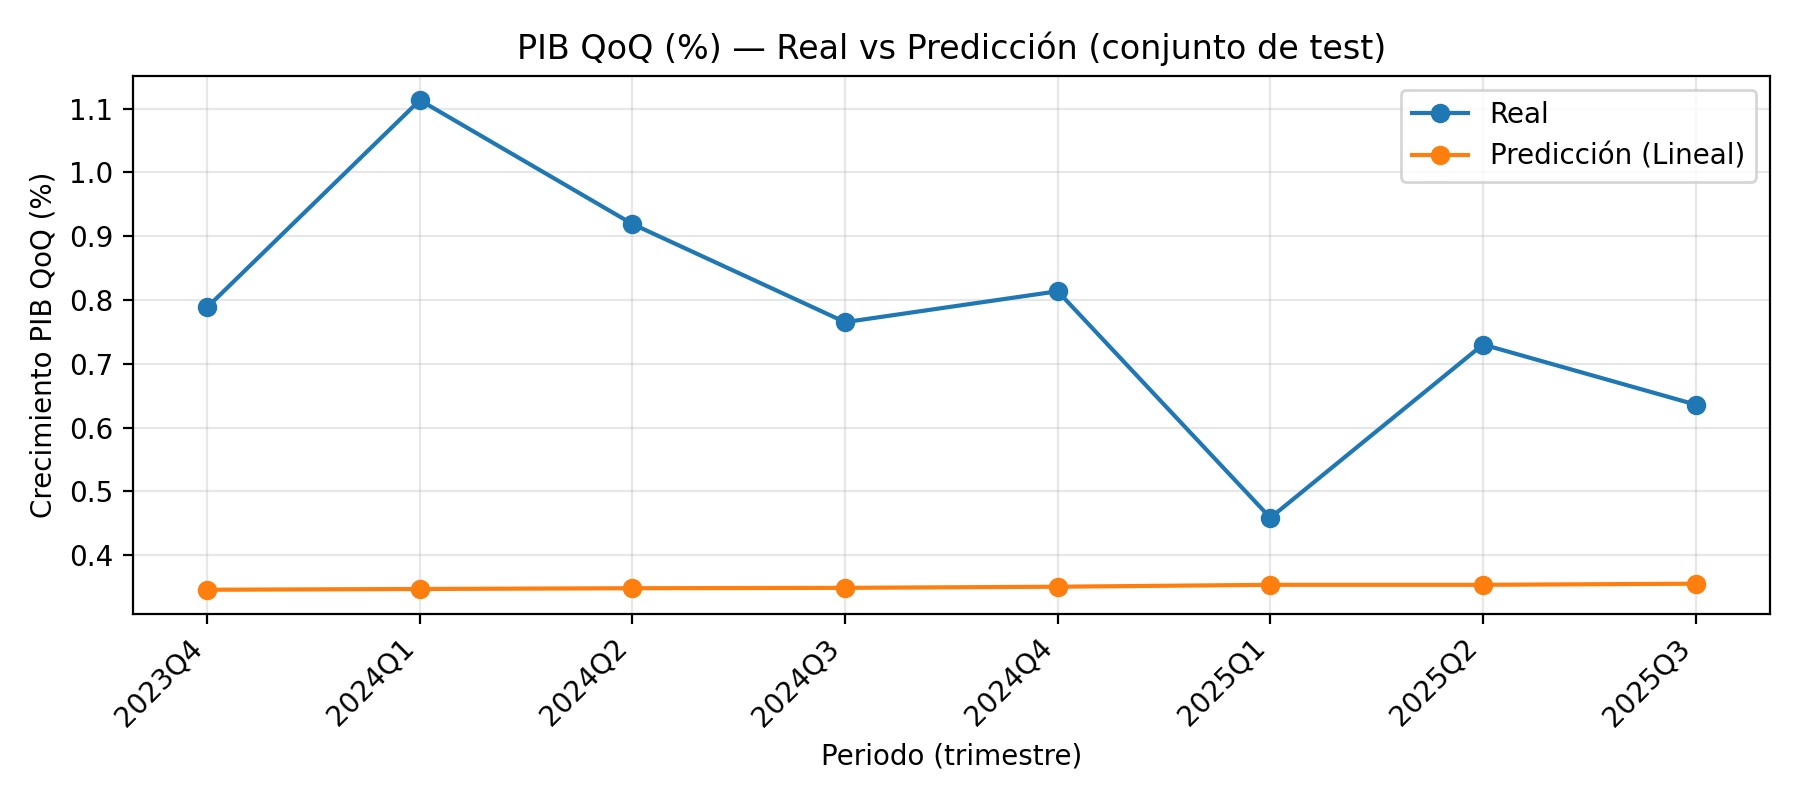
\includegraphics[width=\textwidth]{figures/linear_es_real_vs_pred.png}
    \caption{PIB QoQ real vs predicción -- Lineal univariante (ES, test)}
    \label{fig:lin_es_pred}
\end{minipage}\hfill
\begin{minipage}[t]{0.48\textwidth}
    \centering
    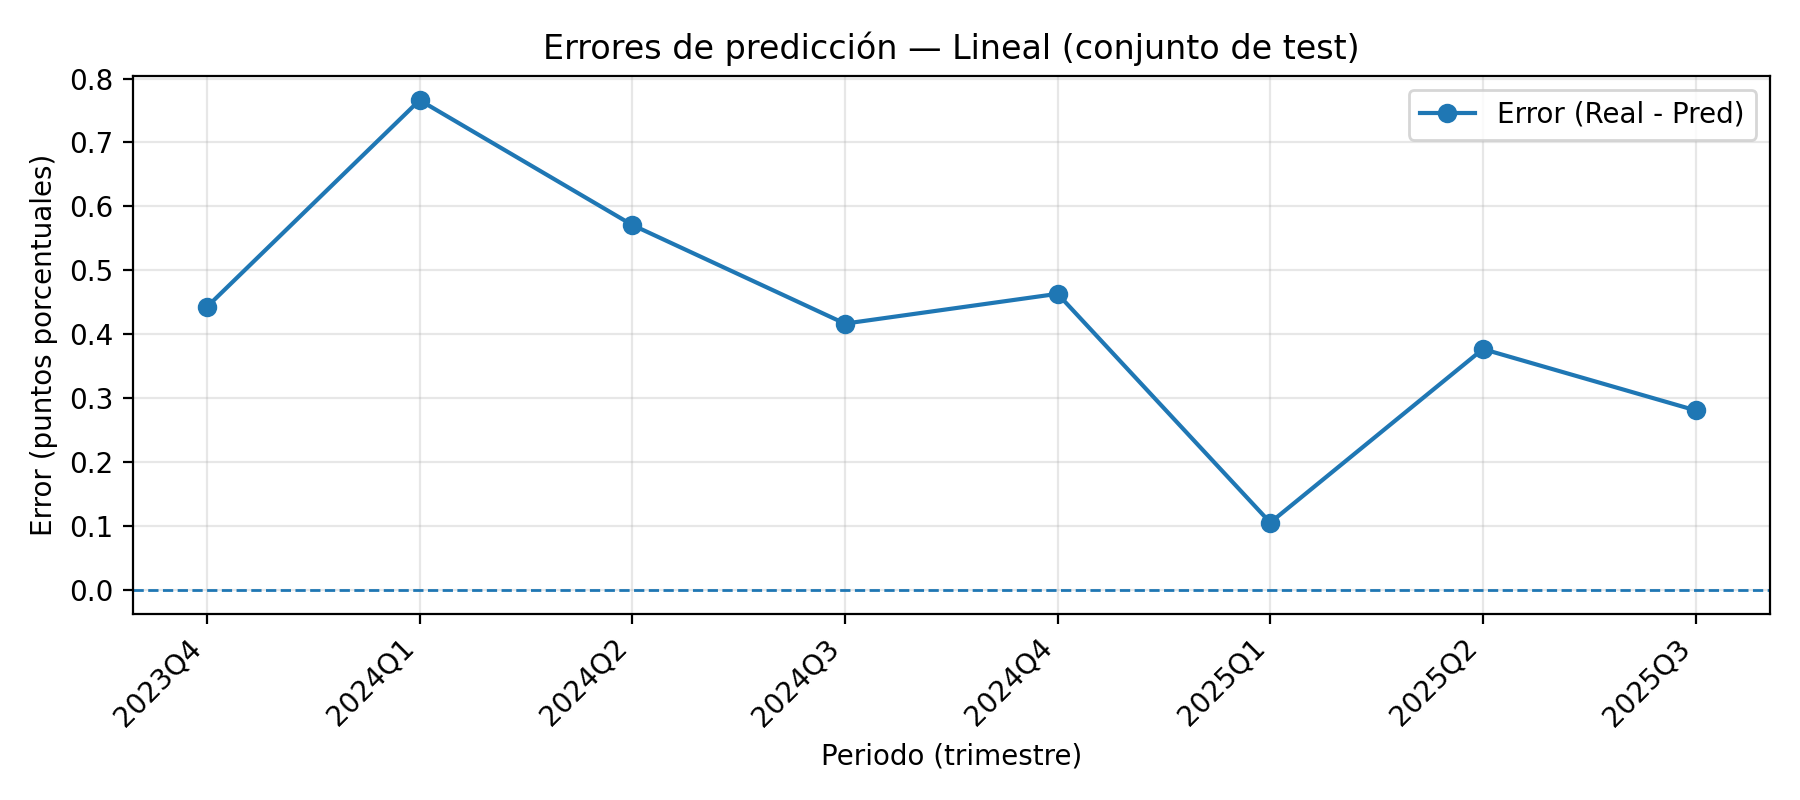
\includegraphics[width=\textwidth]{figures/linear_es_errors.png}
    \caption{Errores de predicción -- Lineal univariante (ES, test)}
    \label{fig:lin_es_err}
\end{minipage}
\end{figure}

\subsection{Modelo multivariante}

El segundo modelo añade la inflación trimestral rezagada como segunda variable predictora:

\[
\widehat{\text{gdp\_qoq\_pct}}_t = \beta_0 + \beta_1 \cdot \text{unemployment\_rate}_{t-1}
+ \beta_2 \cdot \text{inflation\_qoq\_pct}_{t-1}
\]

Contra lo que cabría esperar, los resultados empeoran: MAE = 0.476 p.p. y RMSE = 0.578 p.p.,
frente a los 0.428 y 0.465 del modelo univariante.

La causa reside en la naturaleza de la relación entre inflación y PIB: no es lineal ni
estable en el tiempo. Durante periodos de baja inflación, el crecimiento y la inflación
pueden moverse en la misma dirección; durante periodos de choque de precios como 2022--2023,
la relación se invierte. Un modelo OLS estima un único coeficiente $\beta_2$ promediando
estas fases opuestas, lo que introduce ruido en lugar de señal. La Figura~\ref{fig:lin_multivar_pred}
muestra que la incorporación de la inflación provoca mayor volatilidad en las predicciones
---visible en los errores de la Figura~\ref{fig:lin_multivar_err}---, con un error puntual
de 0.92 p.p. en 2024Q4, trimestre en que la inflación rezagada tomó un valor negativo
inusual que el modelo interpretó erróneamente como señal contractiva.

\begin{figure}[H]
\centering
\begin{minipage}[t]{0.48\textwidth}
    \centering
    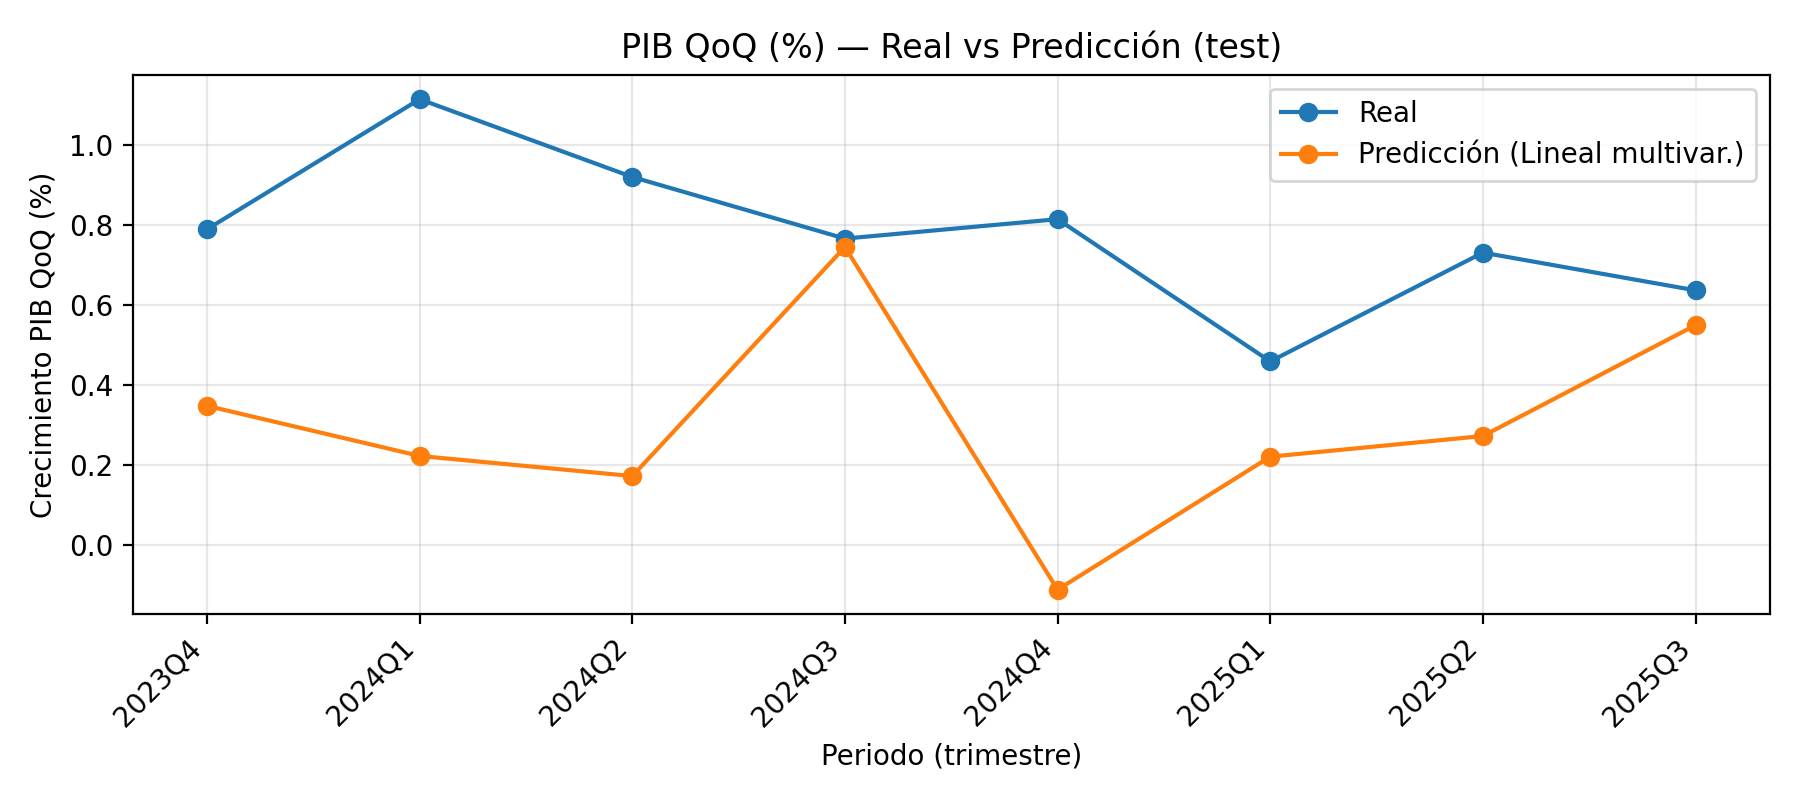
\includegraphics[width=\textwidth]{figures/linear_multivar_es_real_vs_pred.png}
    \caption{PIB QoQ real vs predicción -- Lineal multivariante (ES, test)}
    \label{fig:lin_multivar_pred}
\end{minipage}\hfill
\begin{minipage}[t]{0.48\textwidth}
    \centering
    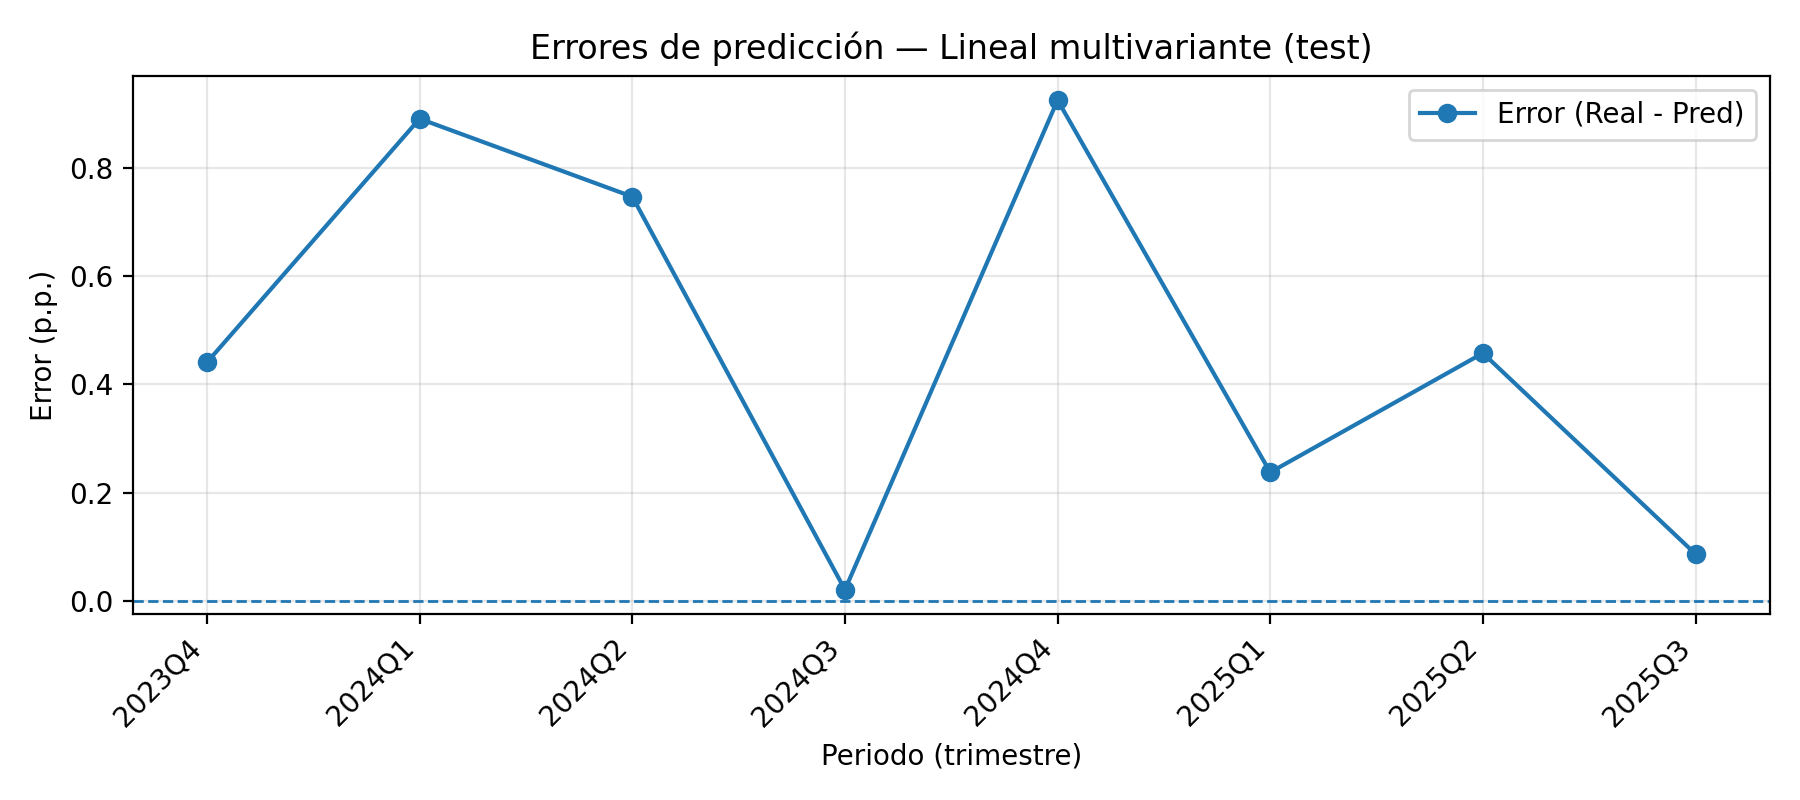
\includegraphics[width=\textwidth]{figures/linear_multivar_es_errors.png}
    \caption{Errores de predicción -- Lineal multivariante (ES, test)}
    \label{fig:lin_multivar_err}
\end{minipage}
\end{figure}

\subsection{Síntesis y comparación con el modelo de referencia}

\begin{table}[H]
\centering
\caption{Resultados de los modelos de regresión lineal -- España}
\label{tab:linear}
\small
\begin{tabular}{lccc}
\hline
\textbf{Modelo} & \textbf{Features} & \textbf{MAE} & \textbf{RMSE} \\
\hline
Lineal univariante   & 1 & 0.428 & 0.465 \\
Lineal multivariante & 2 & 0.476 & 0.578 \\
\hline
\end{tabular}
\end{table}

El análisis revela dos limitaciones estructurales de la regresión lineal para este problema.
Primera: con pocas variables y una relación débil o inestable con el PIB, el modelo tiende
a predecir un valor casi constante próximo a la media de entrenamiento, incapaz de capturar
la variabilidad trimestral real. Segunda: añadir variables no mejora necesariamente el
resultado si la relación con el objetivo no es lineal y estable en el tiempo; en ese caso,
el coeficiente estimado promedia fases de signo opuesto y degrada la predicción.

Estos resultados motivan el uso de XGBoost, que puede capturar relaciones no lineales entre
las variables y el PIB, adaptar su respuesta según el nivel de las variables (lo que OLS
no puede hacer con un único coeficiente), y aprovechar combinaciones de indicadores sin
imponer una forma funcional rígida. Los experimentos de los Bloques 0--2 apuntan a que
este salto en complejidad se traduce en una mejora del error de predicción en la mayor parte de los escenarios analizados.

% ══════════════════════════════════════════════════════════════════════
\FloatBarrier
\section{Bloque 0 --- Modelos por país}

\textbf{Idea principal:} entrenar modelos independientes por país permite establecer una línea de referencia, y los resultados sugieren que no existe una configuración universalmente mejor: la configuración óptima parece depender de la economía analizada, lo que apunta a diferencias estructurales en la predictibilidad del ciclo de cada país.

El primer bloque de experimentos entrena y evalúa los modelos de forma independiente para cada país, utilizando únicamente los datos propios de cada economía. Este enfoque permite establecer los resultados de referencia para cada país antes de explorar estrategias que combinen información de múltiples economías.

Los resultados obtenidos en el conjunto de prueba para los tres países son los siguientes:

\begin{table}[H]
\centering
\caption{Comparativa de modelos XGBoost por país -- Bloque 0}
\label{tab:bloque0}
\small
\begin{tabular}{lcccccc}
\hline
 & \multicolumn{2}{c}{\textbf{España}} & \multicolumn{2}{c}{\textbf{Francia}} & \multicolumn{2}{c}{\textbf{Italia}} \\
\textbf{Modelo} & \textbf{MAE} & \textbf{RMSE} & \textbf{MAE} & \textbf{RMSE} & \textbf{MAE} & \textbf{RMSE} \\
\hline
XGBoost base     & 0.314 & 0.365 & 0.441 & 0.486 & 0.761 & 0.813 \\
XGBoost ampliado & 0.796 & 1.285 & 0.193 & 0.208 & 0.344 & 0.455 \\
\hline
\end{tabular}
\end{table}

\FloatBarrier
\subsection{España}

El modelo base obtiene el mejor resultado para España (MAE 0.314), superando claramente al modelo ampliado (MAE 0.796). Como se observa en la Figura~\ref{fig:xgb_base_es}, el modelo base reproduce razonablemente la tendencia del crecimiento trimestral, manteniéndose en el rango positivo y siguiendo de forma aproximada la evolución real.

En cambio, la Figura~\ref{fig:xgb_ext_es} muestra que el modelo ampliado produce una predicción anómala de $-2.5$ puntos porcentuales en 2023Q4, cuando el valor real fue de $0.8$ p.p. Este error en el primer trimestre del conjunto de prueba es el principal responsable del alto RMSE del modelo ampliado, y apunta a un problema de sobreajuste sobre los retardos del PIB durante el entrenamiento.

\begin{figure}[H]
\centering
\begin{minipage}[t]{0.48\textwidth}
    \centering
    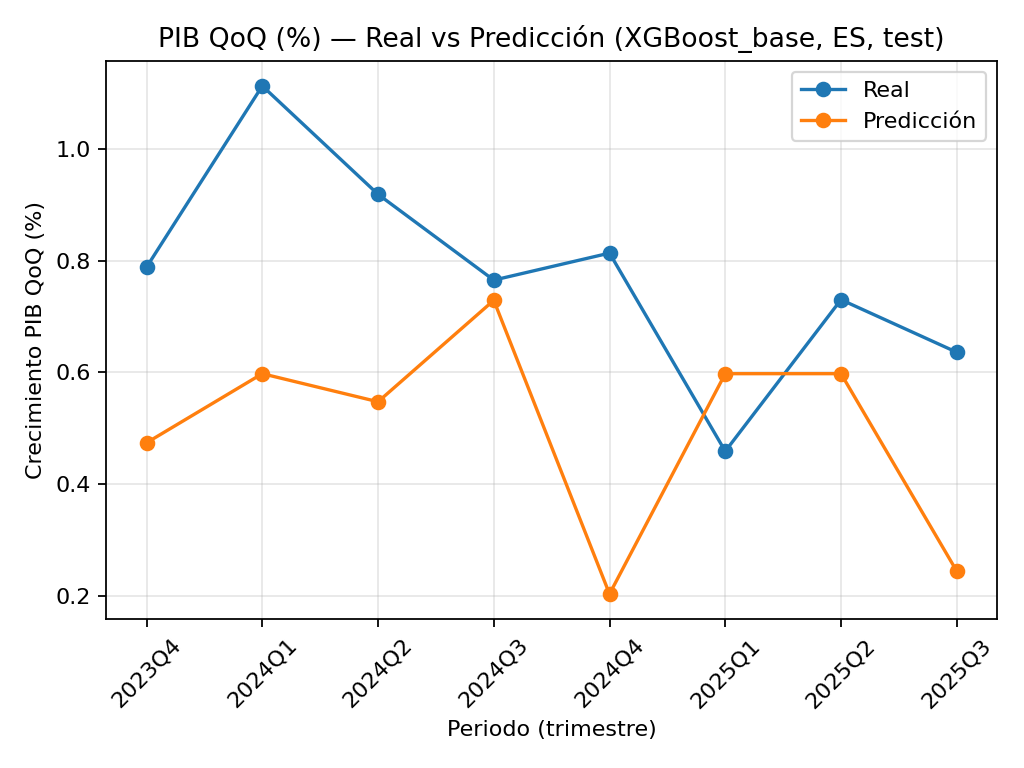
\includegraphics[width=\textwidth]{figures/bloque 0/xgboost_base_es_real_vs_pred.png}
    \caption{PIB QoQ real vs predicción -- XGBoost base (ES, test)}
    \label{fig:xgb_base_es}
\end{minipage}\hfill
\begin{minipage}[t]{0.48\textwidth}
    \centering
    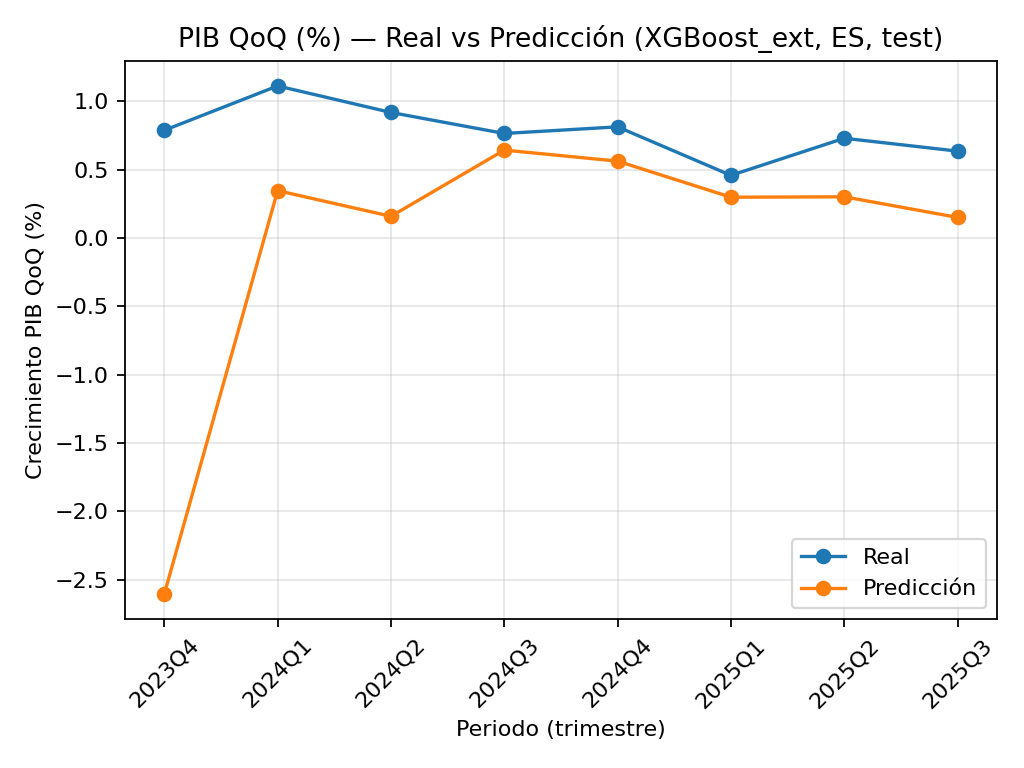
\includegraphics[width=\textwidth]{figures/bloque 0/xgboost_ext_es_real_vs_pred.png}
    \caption{PIB QoQ real vs predicción -- XGBoost ampliado (ES, test)}
    \label{fig:xgb_ext_es}
\end{minipage}
\end{figure}

\FloatBarrier
\subsection{Francia}

Francia presenta el patrón opuesto: el modelo ampliado (MAE 0.193) supera con claridad al modelo base (MAE 0.441). La Figura~\ref{fig:xgb_base_fr} muestra que el modelo base oscila de forma pronunciada alrededor de los valores reales sin capturar bien la tendencia. El modelo ampliado, visible en la Figura~\ref{fig:xgb_ext_fr}, sigue de forma más suave la evolución real, aunque tiende a sobreestimar ligeramente el crecimiento en los trimestres centrales del periodo de prueba.

\begin{figure}[H]
\centering
\begin{minipage}[t]{0.48\textwidth}
    \centering
    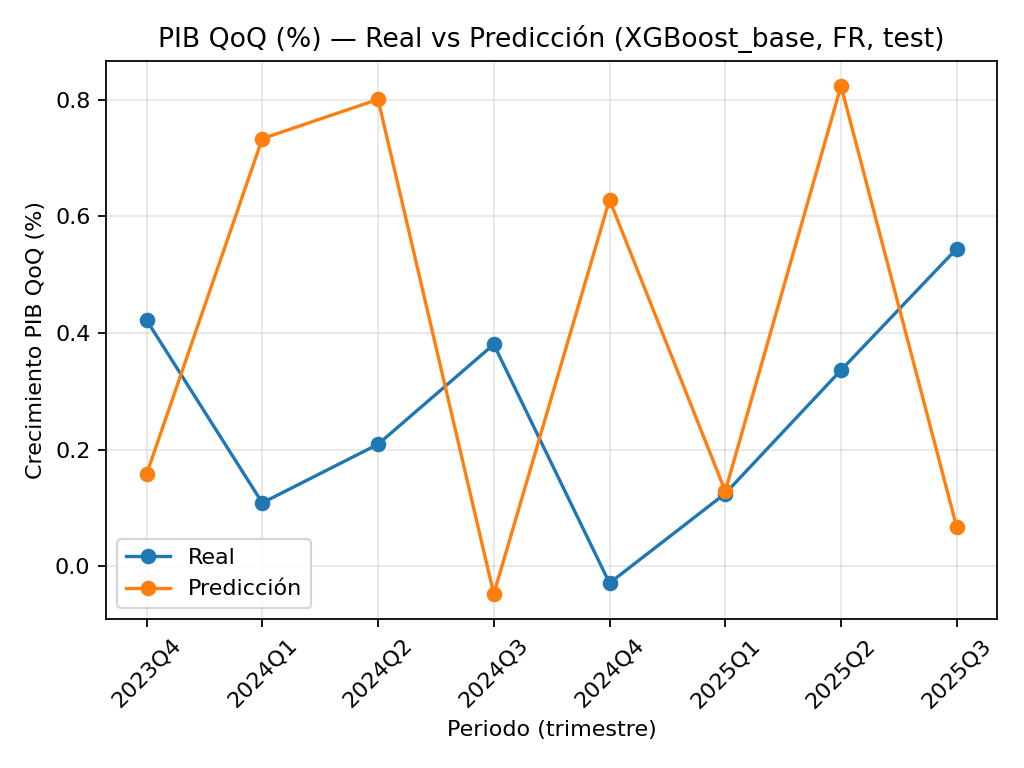
\includegraphics[width=\textwidth]{figures/bloque 0/xgboost_base_fr_real_vs_pred.png}
    \caption{PIB QoQ real vs predicción -- XGBoost base (FR, test)}
    \label{fig:xgb_base_fr}
\end{minipage}\hfill
\begin{minipage}[t]{0.48\textwidth}
    \centering
    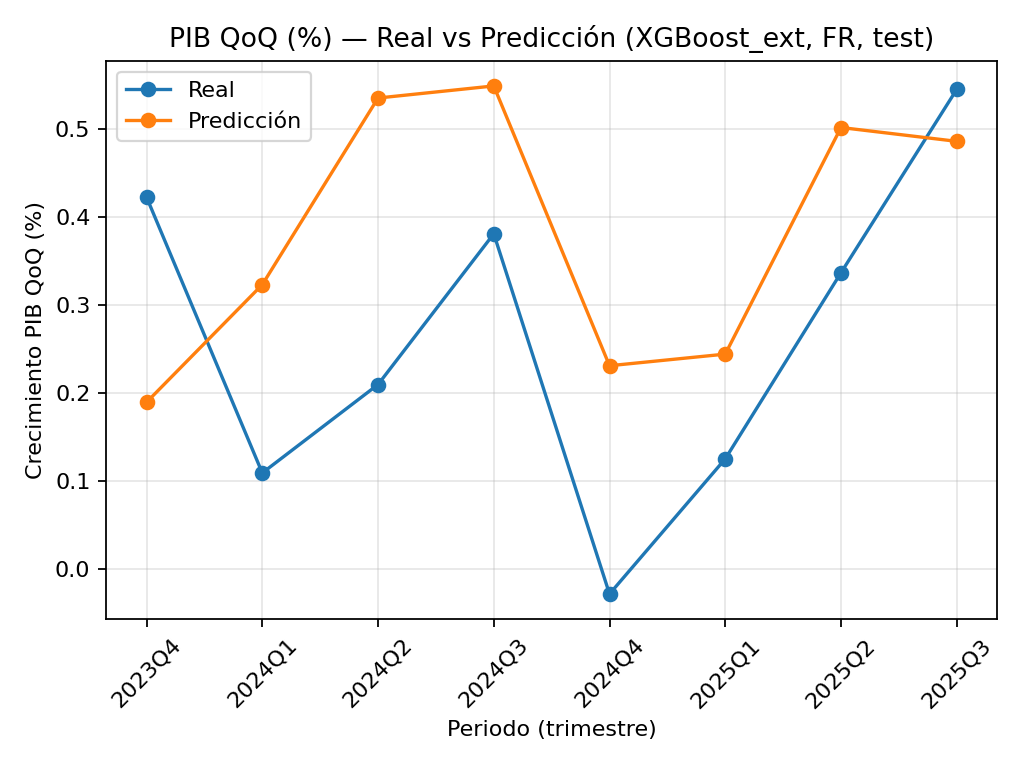
\includegraphics[width=\textwidth]{figures/bloque 0/xgboost_ext_fr_real_vs_pred.png}
    \caption{PIB QoQ real vs predicción -- XGBoost ampliado (FR, test)}
    \label{fig:xgb_ext_fr}
\end{minipage}
\end{figure}

\FloatBarrier
\subsection{Italia}

Italia es el país con mayor error en el modelo base (MAE 0.761), con predicciones que se alejan notablemente de los valores reales en varios trimestres, como se aprecia en la Figura~\ref{fig:xgb_base_it}. El modelo ampliado mejora considerablemente (MAE 0.344), aunque la Figura~\ref{fig:xgb_ext_it} muestra una predicción anómala de $-0.85$ p.p. en 2024Q2 cuando el valor real fue de $0.2$ p.p., patrón similar al observado en España con el modelo ampliado.

\begin{figure}[H]
\centering
\begin{minipage}[t]{0.48\textwidth}
    \centering
    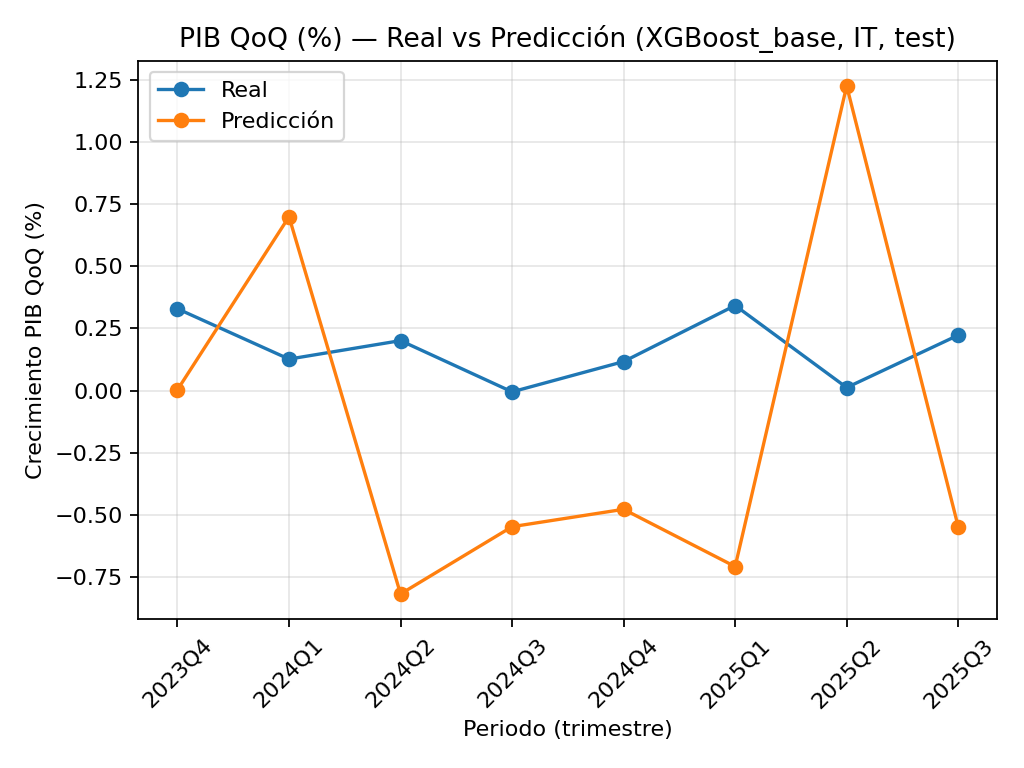
\includegraphics[width=\textwidth]{figures/bloque 0/xgboost_base_it_real_vs_pred.png}
    \caption{PIB QoQ real vs predicción -- XGBoost base (IT, test)}
    \label{fig:xgb_base_it}
\end{minipage}\hfill
\begin{minipage}[t]{0.48\textwidth}
    \centering
    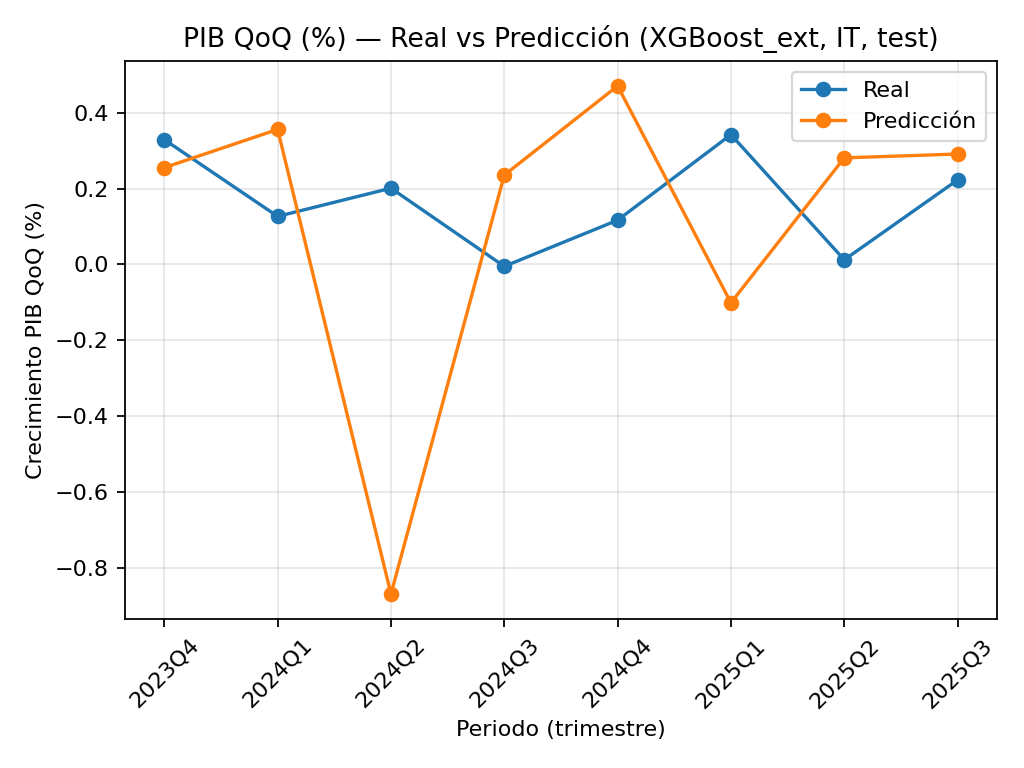
\includegraphics[width=\textwidth]{figures/bloque 0/xgboost_ext_it_real_vs_pred.png}
    \caption{PIB QoQ real vs predicción -- XGBoost ampliado (IT, test)}
    \label{fig:xgb_ext_it}
\end{minipage}
\end{figure}

\FloatBarrier
\subsection{Importancia de variables}

Las Figuras~\ref{fig:feat_es}, \ref{fig:feat_fr} y~\ref{fig:feat_it} muestran la importancia relativa de las variables según el criterio de ganancia (\textit{gain}) del modelo ampliado para cada país. En los tres casos el retardo inmediato del PIB (\texttt{gdp\_\allowbreak{}qoq\_\allowbreak{}pct\_\allowbreak{}l1}) concentra la mayor parte de la importancia explicativa, seguido a distancia por el índice de producción industrial y el comercio minorista. El desempleo y la inflación rezagados presentan una contribución marginal en los tres países, lo que sugiere que su capacidad predictiva a un trimestre vista es limitada en el periodo analizado.

\begin{figure}[H]
\centering
\begin{minipage}[t]{0.48\textwidth}
    \centering
    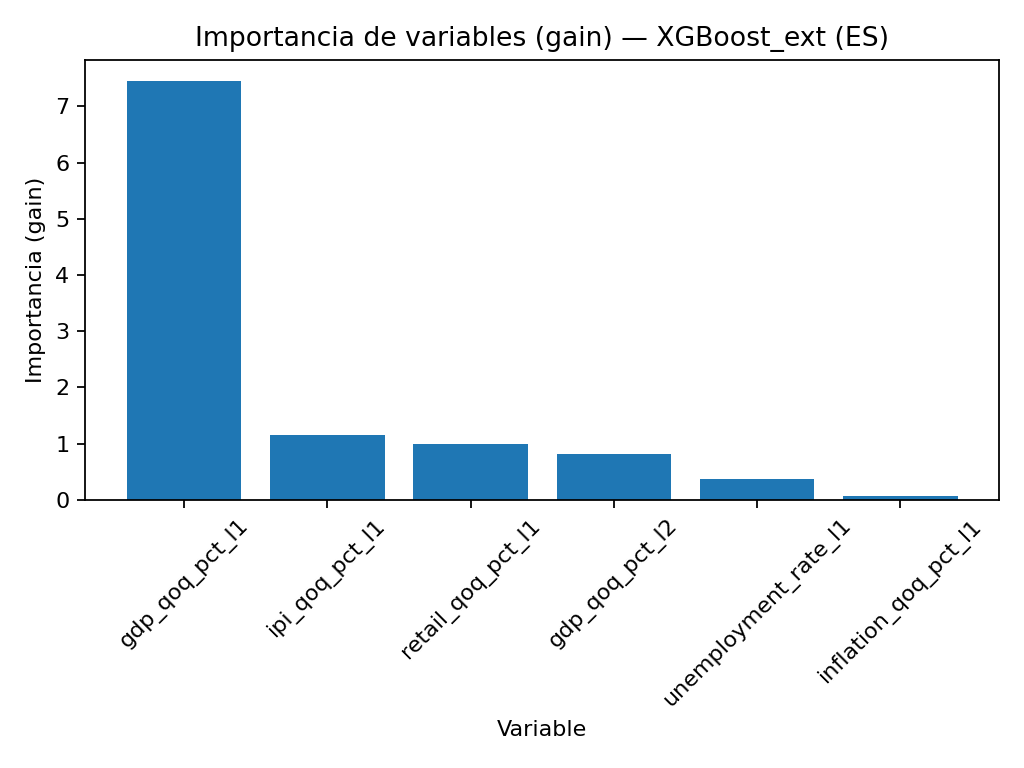
\includegraphics[width=\textwidth]{figures/bloque 0/xgboost_ext_es_feature_importance.png}
    \caption{Importancia de variables (gain) -- XGBoost ampliado (ES)}
    \label{fig:feat_es}
\end{minipage}\hfill
\begin{minipage}[t]{0.48\textwidth}
    \centering
    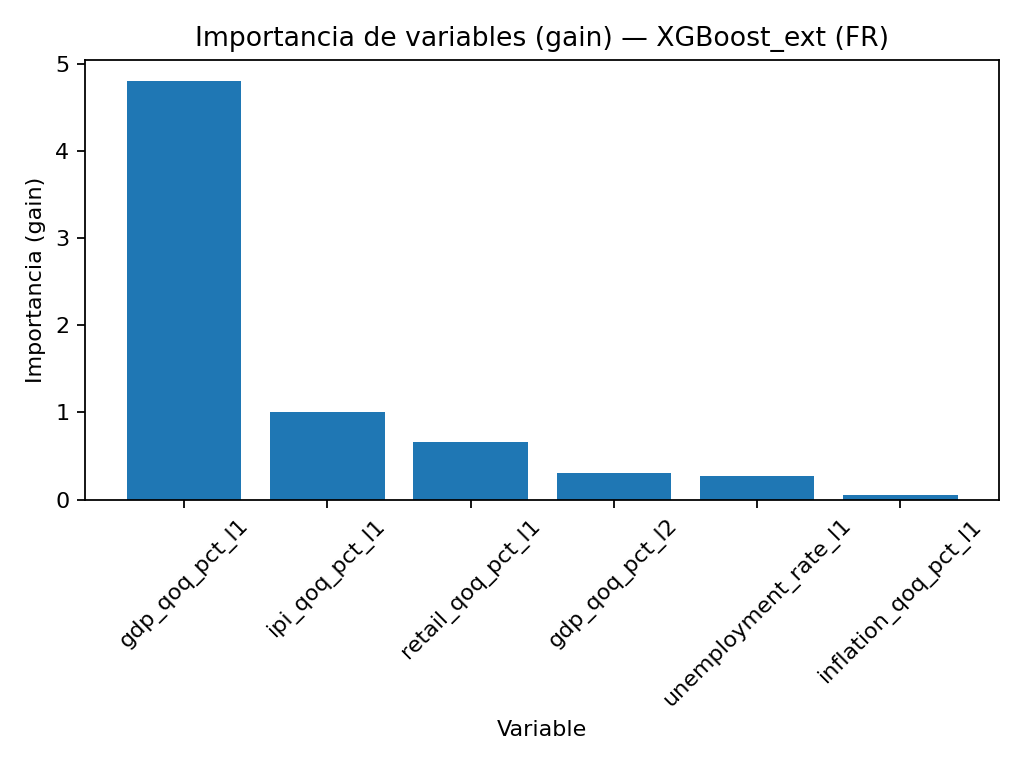
\includegraphics[width=\textwidth]{figures/bloque 0/xgboost_ext_fr_feature_importance.png}
    \caption{Importancia de variables (gain) -- XGBoost ampliado (FR)}
    \label{fig:feat_fr}
\end{minipage}
\end{figure}

\begin{figure}[H]
\centering
\begin{minipage}[t]{0.48\textwidth}
    \centering
    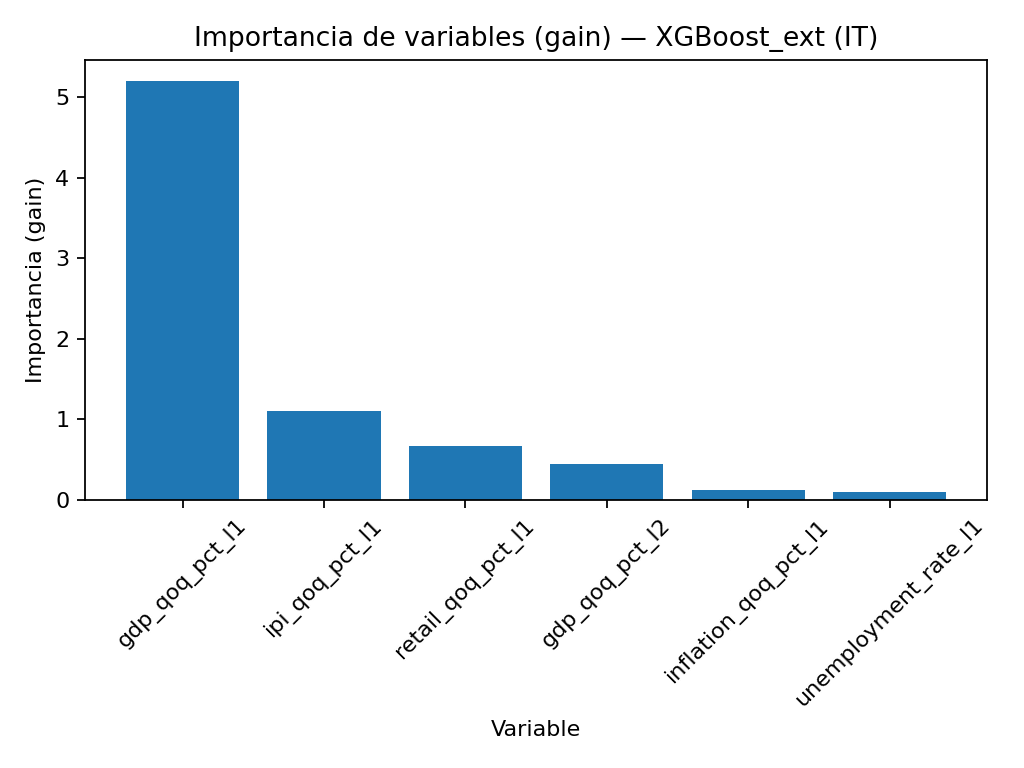
\includegraphics[width=\textwidth]{figures/bloque 0/xgboost_ext_it_feature_importance.png}
    \caption{Importancia de variables (gain) -- XGBoost ampliado (IT)}
    \label{fig:feat_it}
\end{minipage}
\end{figure}

\FloatBarrier
\subsection{Síntesis del Bloque 0}

El análisis por país revela que no existe un modelo universalmente mejor: la configuración óptima depende de la economía analizada. En España, el modelo base ofrece un mejor equilibrio entre simplicidad y capacidad de generalización, mientras que Francia e Italia se benefician de la incorporación de variables adicionales.

Este resultado sugiere que la dinámica del crecimiento económico español presenta una componente autorregresiva más débil en el periodo de prueba, de modo que añadir los retardos del propio PIB no aporta información útil y aumenta el riesgo de sobreajuste. En cambio, para Francia e Italia la incorporación de los retardos del PIB y de los indicadores de actividad económica sí mejora la capacidad predictiva, lo que indica que la dinámica de estas economías es más persistente o que los indicadores de actividad adelantan mejor el crecimiento futuro.

Adicionalmente, se observa una diferencia notable en la dificultad de predicción entre países con el modelo base: España presenta el error más bajo (MAE 0.314), seguida de Francia (0.441) e Italia (0.761), lo que apunta a diferencias estructurales en la predictibilidad del ciclo económico de cada país. Estos resultados motivan la exploración de estrategias que combinen información de múltiples países, abordada en los bloques experimentales siguientes.

% ══════════════════════════════════════════════════════════════════════
\FloatBarrier
\section{Bloque 1 --- Modelo panel combinado}

\textbf{Idea principal:} combinar los datos de los tres países en un único modelo parece reducir el sobreajuste observado en el Bloque~0, siendo el efecto más llamativo la recuperación del modelo ampliado para España (de MAE 0.796 a 0.297). El modelo panel ampliado parece ser la configuración más robusta del bloque, obteniendo resultados competitivos en los tres países de forma simultánea.

El segundo bloque de experimentos entrena un único modelo XGBoost utilizando los datos de los tres países de forma conjunta, evaluando posteriormente el rendimiento de forma separada para cada economía. A diferencia del Bloque~0, donde cada modelo solo disponía de las observaciones de su propio país (aproximadamente 58 trimestres por economía), aquí el modelo de entrenamiento accede a las ~174 observaciones combinadas del panel completo.

El objetivo de este enfoque es doble. Por un lado, aumentar el volumen de datos de entrenamiento para reducir el riesgo de sobreajuste, problema que afectó especialmente al modelo ampliado de España en el Bloque~0. Por otro, comprobar si los patrones macroeconómicos son suficientemente comunes entre las tres economías como para que un modelo compartido generalice mejor que tres modelos independientes.

Los resultados obtenidos en el conjunto de prueba son los siguientes:

\begin{table}[H]
\centering
\caption{Comparativa de modelos panel combinado por país -- Bloque 1}
\label{tab:bloque1}
\small
\begin{tabular}{lcccccc}
\hline
 & \multicolumn{2}{c}{\textbf{España}} & \multicolumn{2}{c}{\textbf{Francia}} & \multicolumn{2}{c}{\textbf{Italia}} \\
\textbf{Modelo} & \textbf{MAE} & \textbf{RMSE} & \textbf{MAE} & \textbf{RMSE} & \textbf{MAE} & \textbf{RMSE} \\
\hline
panel\_combined\_base & 0.363 & 0.462 & 0.316 & 0.426 & 0.631 & 1.039 \\
panel\_combined\_ext  & 0.297 & 0.331 & 0.215 & 0.256 & 0.376 & 0.466 \\
\hline
\end{tabular}
\end{table}

Comparando con los resultados del Bloque~0 (Tabla~\ref{tab:bloque0}), el modelo panel muestra mejoras generalizadas en el modelo ampliado y un comportamiento más consistente entre países, como se analiza en las subsecciones siguientes.

\FloatBarrier
\subsection{España}

España es el país donde el cambio de estrategia produce el impacto más destacado. El modelo ampliado, que en el Bloque~0 presentaba el peor resultado para esta economía (MAE 0.796) debido a una predicción anómala de $-2.5$ p.p. en 2023Q4, pasa ahora a obtener el mejor resultado con MAE 0.297, superando incluso al modelo base del panel (MAE 0.363).

Este resultado apunta al efecto regularizador del mayor volumen de datos: al entrenar con las observaciones combinadas de los tres países, el modelo ampliado parece dejar de memorizar los retardos del PIB español y adquiere una mayor capacidad de generalización. Las Figuras~\ref{fig:panel_base_es_pred} y~\ref{fig:panel_ext_es_pred} permiten apreciar visualmente esta mejora. El modelo base del panel (Figura~\ref{fig:panel_base_es_pred}) sigue con dificultad la aceleración del crecimiento español en 2024Q1 y tiende a subestimar los trimestres finales del periodo de prueba. El modelo ampliado del panel (Figura~\ref{fig:panel_ext_es_pred}), en cambio, captura mejor la tendencia general, aunque sobreestima el pico de 2024Q3 y no anticipa la moderación posterior.

Los errores de predicción, representados en las Figuras~\ref{fig:panel_base_es_err} y~\ref{fig:panel_ext_es_err}, muestran que ambos modelos producen errores de signo variable sin un sesgo sistemático claro. El modelo ampliado presenta errores más contenidos y distribuidos de forma más homogénea a lo largo del periodo de prueba, mientras que el modelo base acumula errores positivos crecientes hacia el final del horizonte.

\begin{figure}[H]
\centering
\begin{minipage}[t]{0.48\textwidth}
    \centering
    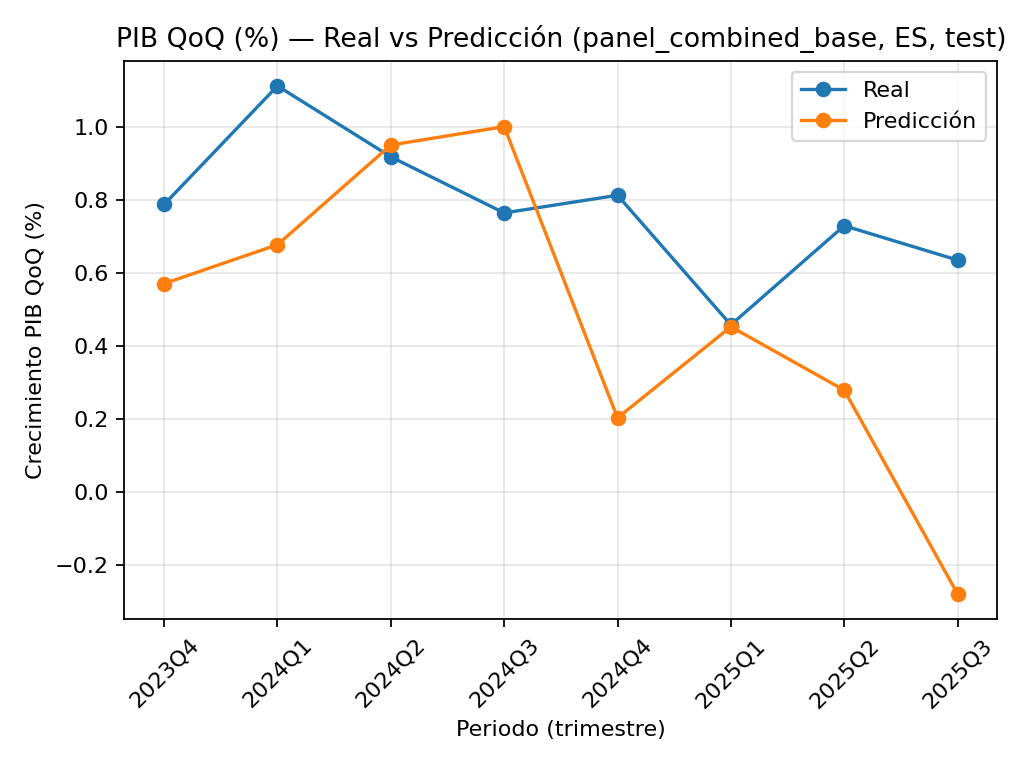
\includegraphics[width=\textwidth]{figures/bloque 1/panel_combined_base_es_real_vs_pred.png}
    \caption{PIB QoQ real vs predicción -- panel combinado base (ES, test)}
    \label{fig:panel_base_es_pred}
\end{minipage}\hfill
\begin{minipage}[t]{0.48\textwidth}
    \centering
    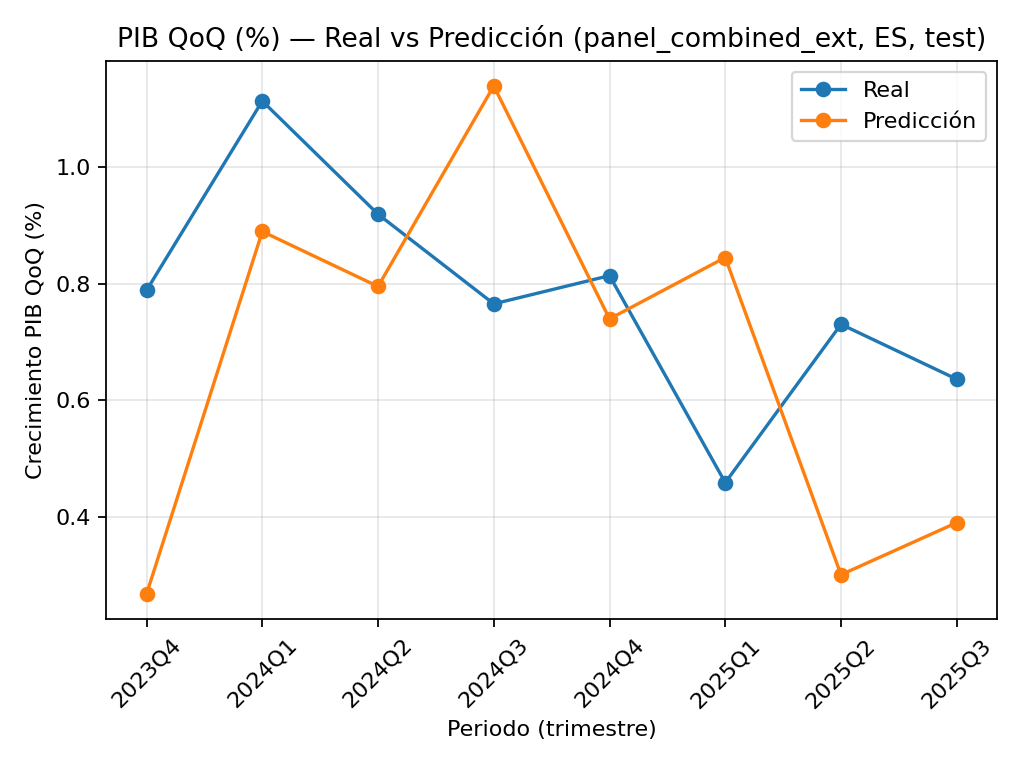
\includegraphics[width=\textwidth]{figures/bloque 1/panel_combined_ext_es_real_vs_pred.png}
    \caption{PIB QoQ real vs predicción -- panel combinado ampliado (ES, test)}
    \label{fig:panel_ext_es_pred}
\end{minipage}

\vspace{0.5em}

\begin{minipage}[t]{0.48\textwidth}
    \centering
    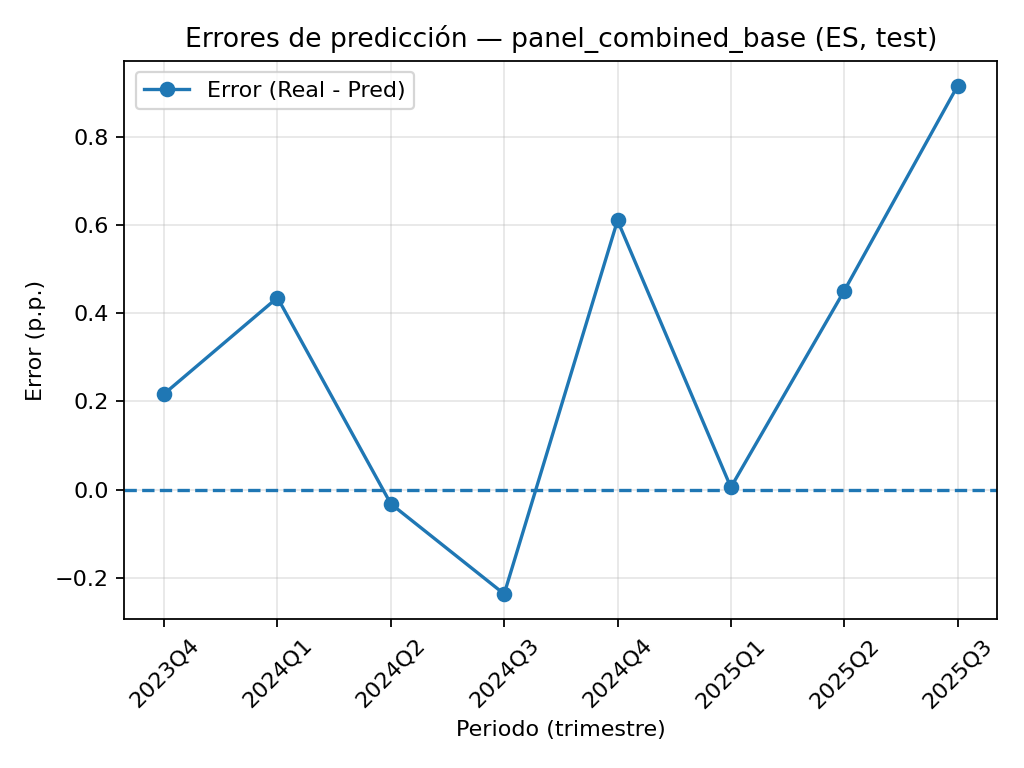
\includegraphics[width=\textwidth]{figures/bloque 1/panel_combined_base_es_errors.png}
    \caption{Errores de predicción -- panel combinado base (ES, test)}
    \label{fig:panel_base_es_err}
\end{minipage}\hfill
\begin{minipage}[t]{0.48\textwidth}
    \centering
    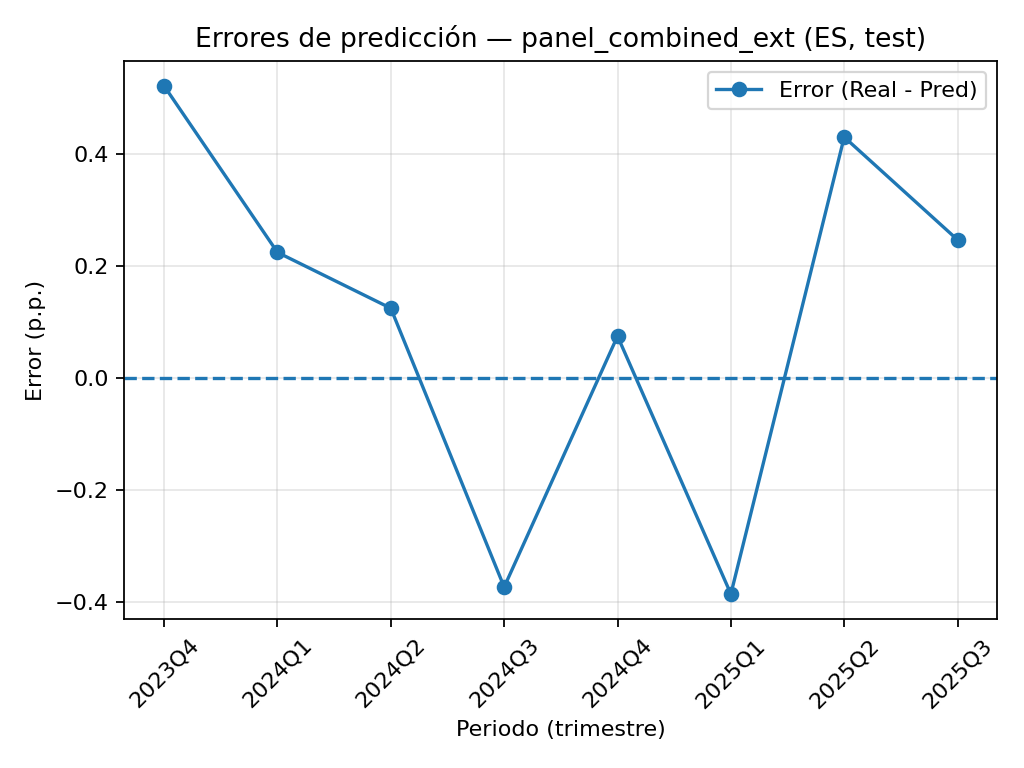
\includegraphics[width=\textwidth]{figures/bloque 1/panel_combined_ext_es_errors.png}
    \caption{Errores de predicción -- panel combinado ampliado (ES, test)}
    \label{fig:panel_ext_es_err}
\end{minipage}
\end{figure}

\FloatBarrier
\subsection{Francia}

Francia confirma los buenos resultados ya obtenidos en el Bloque~0 y los mejora en ambas configuraciones. El modelo ampliado reduce su MAE de 0.193 a 0.215 --- una diferencia mínima que puede atribuirse a variabilidad muestral ---, mientras que el modelo base mejora notablemente, pasando de MAE 0.441 a 0.316. Este resultado indica que el panel conjunto es especialmente beneficioso para la configuración base, que en el Bloque~0 carecía de suficiente señal predictiva con solo dos variables y los datos de un único país.

La Figura~\ref{fig:panel_base_fr_pred} muestra que el modelo base del panel ya no oscila de forma tan pronunciada como en el Bloque~0, sino que sigue con mayor suavidad la evolución real del crecimiento francés. El modelo ampliado (Figura~\ref{fig:panel_ext_fr_pred}) mantiene un ajuste similar al del Bloque~0, con una sobreestimación moderada en 2024Q3 y cierta dificultad para anticipar la caída de 2024Q4, aunque las magnitudes de error son en general contenidas.

Los gráficos de error de las Figuras~\ref{fig:panel_base_fr_err} y~\ref{fig:panel_ext_fr_err} revelan que el error más pronunciado del modelo base se concentra en 2024Q3, donde la predicción se aleja aproximadamente 0.94 p.p. del valor real. El modelo ampliado distribuye mejor los errores a lo largo del periodo, con valores que raramente superan $\pm 0.45$ p.p.

\begin{figure}[H]
\centering
\begin{minipage}[t]{0.48\textwidth}
    \centering
    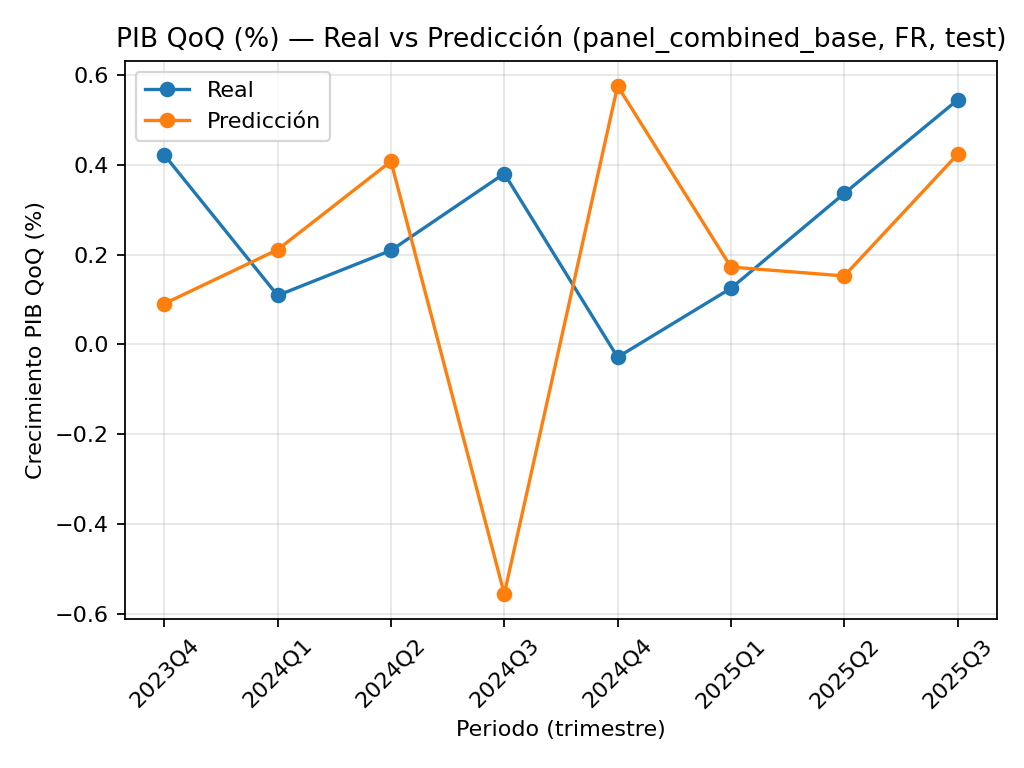
\includegraphics[width=\textwidth]{figures/bloque 1/panel_combined_base_fr_real_vs_pred.png}
    \caption{PIB QoQ real vs predicción -- panel combinado base (FR, test)}
    \label{fig:panel_base_fr_pred}
\end{minipage}\hfill
\begin{minipage}[t]{0.48\textwidth}
    \centering
    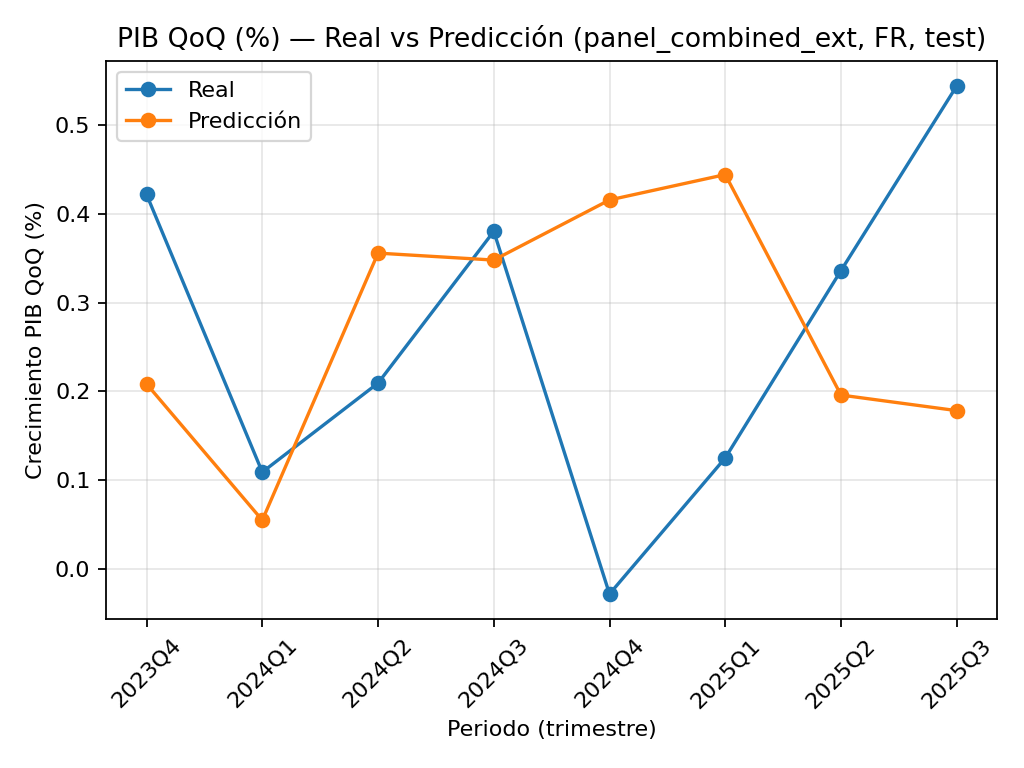
\includegraphics[width=\textwidth]{figures/bloque 1/panel_combined_ext_fr_real_vs_pred.png}
    \caption{PIB QoQ real vs predicción -- panel combinado ampliado (FR, test)}
    \label{fig:panel_ext_fr_pred}
\end{minipage}

\vspace{0.5em}

\begin{minipage}[t]{0.48\textwidth}
    \centering
    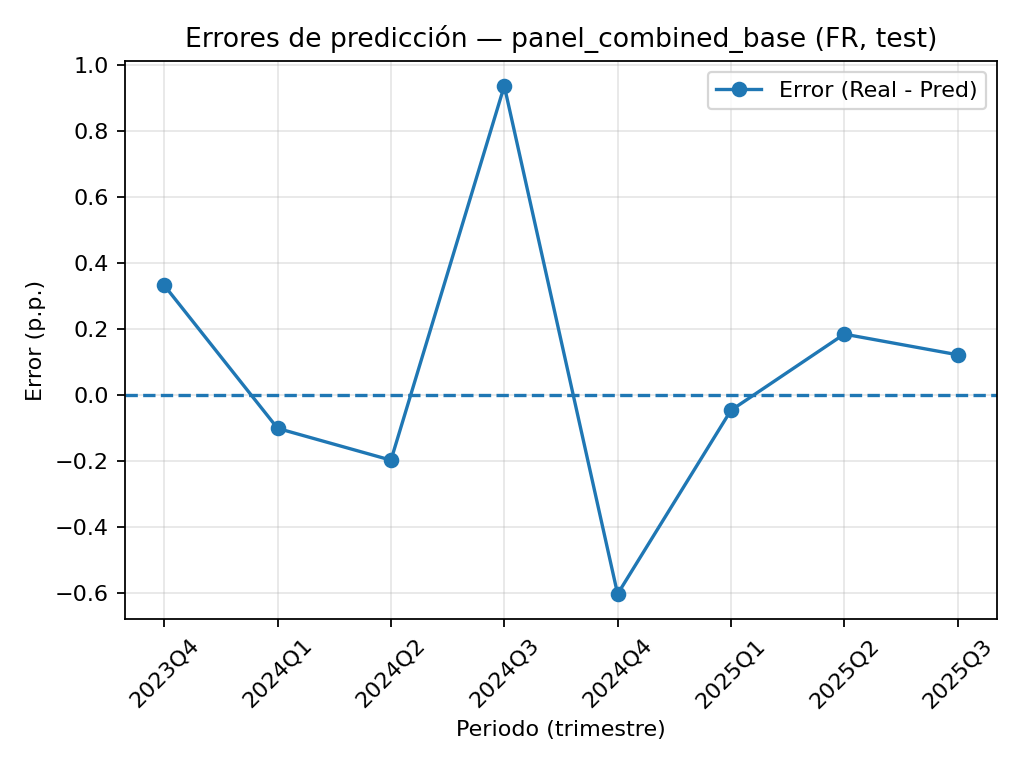
\includegraphics[width=\textwidth]{figures/bloque 1/panel_combined_base_fr_errors.png}
    \caption{Errores de predicción -- panel combinado base (FR, test)}
    \label{fig:panel_base_fr_err}
\end{minipage}\hfill
\begin{minipage}[t]{0.48\textwidth}
    \centering
    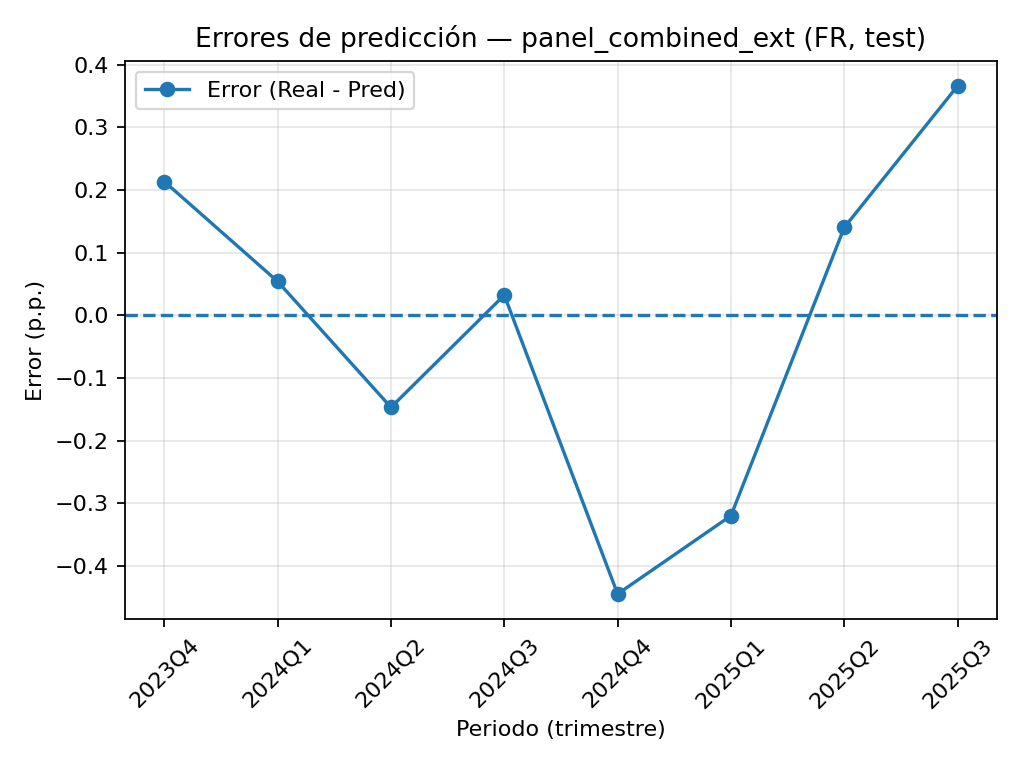
\includegraphics[width=\textwidth]{figures/bloque 1/panel_combined_ext_fr_errors.png}
    \caption{Errores de predicción -- panel combinado ampliado (FR, test)}
    \label{fig:panel_ext_fr_err}
\end{minipage}
\end{figure}

\FloatBarrier
\subsection{Italia}

Italia sigue siendo el país con mayor dificultad de predicción en ambas configuraciones. El modelo base mejora su MAE de 0.761 a 0.631 respecto al Bloque~0, aunque su RMSE asciende a 1.039, el valor más alto de todo el bloque. La gran distancia entre MAE y RMSE delata la presencia de al menos un error puntual muy elevado ---visible en los gráficos de error--- que infla el RMSE sin que el error medio sea tan llamativo. El modelo ampliado presenta un MAE de 0.376, ligeramente superior al 0.344 del Bloque~0, pero con un RMSE de 0.466 que sí mejora el 0.455 anterior, indicando que los errores extremos se han suavizado aunque el error típico haya aumentado marginalmente.

La Figura~\ref{fig:panel_base_it_pred} muestra que el modelo base del panel corrige en parte el comportamiento errático observado en el Bloque~0, donde la predicción llegó a situarse en $-0.07$ p.p. cuando el crecimiento real era de $0.34$ p.p. Aun así, las predicciones siguen sin capturar bien la variabilidad trimestral italiana, que presenta oscilaciones más bruscas que las de España o Francia. El modelo ampliado (Figura~\ref{fig:panel_ext_it_pred}) reproduce mejor la dirección general del crecimiento, aunque los gráficos de error (Figuras~\ref{fig:panel_base_it_err} y~\ref{fig:panel_ext_it_err}) revelan errores puntuales superiores a 0.8 p.p. en 2024Q1 y 2024Q4, trimestres en los que el modelo no anticipa la magnitud de los cambios en la actividad económica italiana.

\begin{figure}[H]
\centering
\begin{minipage}[t]{0.48\textwidth}
    \centering
    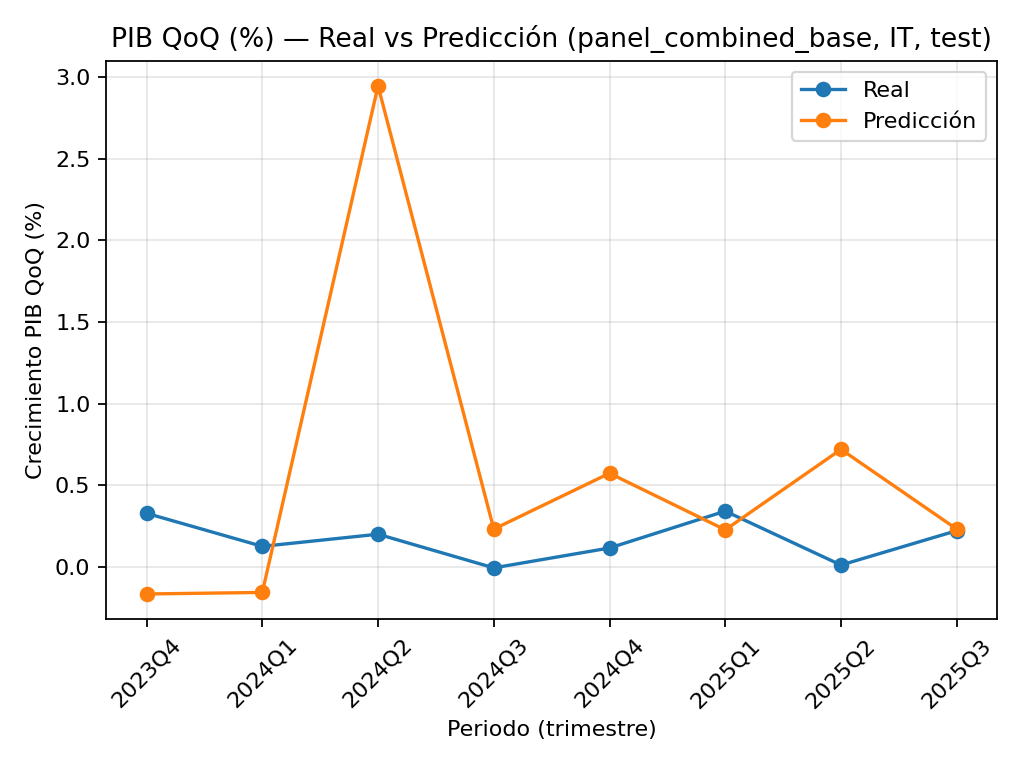
\includegraphics[width=\textwidth]{figures/bloque 1/panel_combined_base_it_real_vs_pred.png}
    \caption{PIB QoQ real vs predicción -- panel combinado base (IT, test)}
    \label{fig:panel_base_it_pred}
\end{minipage}\hfill
\begin{minipage}[t]{0.48\textwidth}
    \centering
    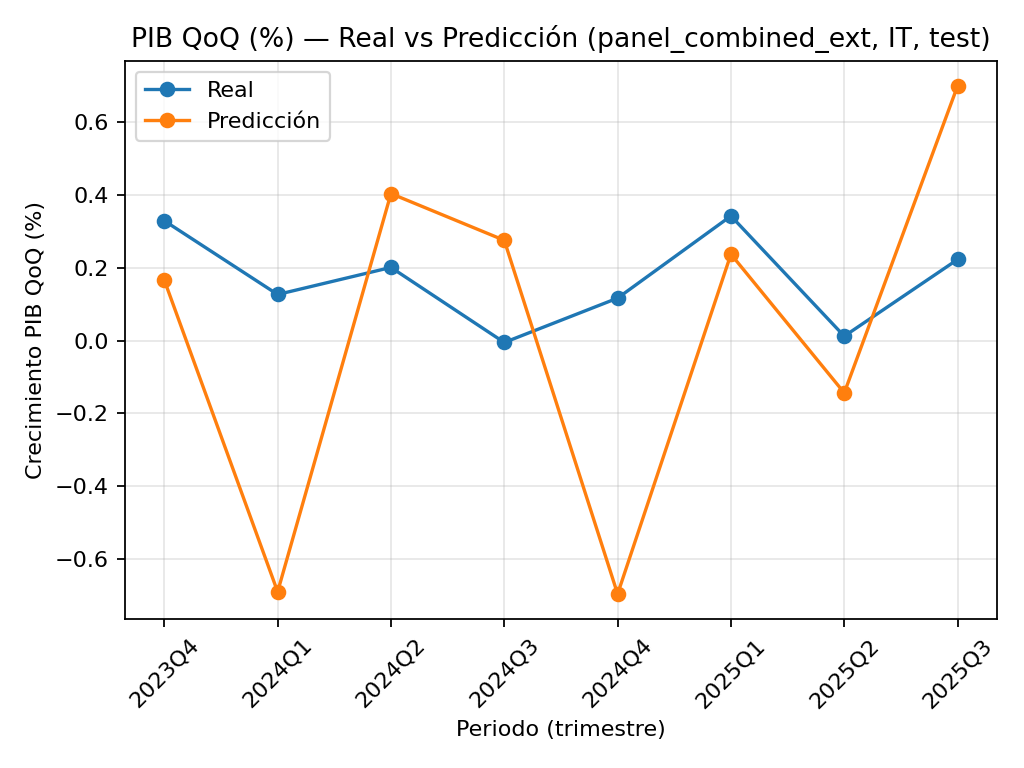
\includegraphics[width=\textwidth]{figures/bloque 1/panel_combined_ext_it_real_vs_pred.png}
    \caption{PIB QoQ real vs predicción -- panel combinado ampliado (IT, test)}
    \label{fig:panel_ext_it_pred}
\end{minipage}

\vspace{0.5em}

\begin{minipage}[t]{0.48\textwidth}
    \centering
    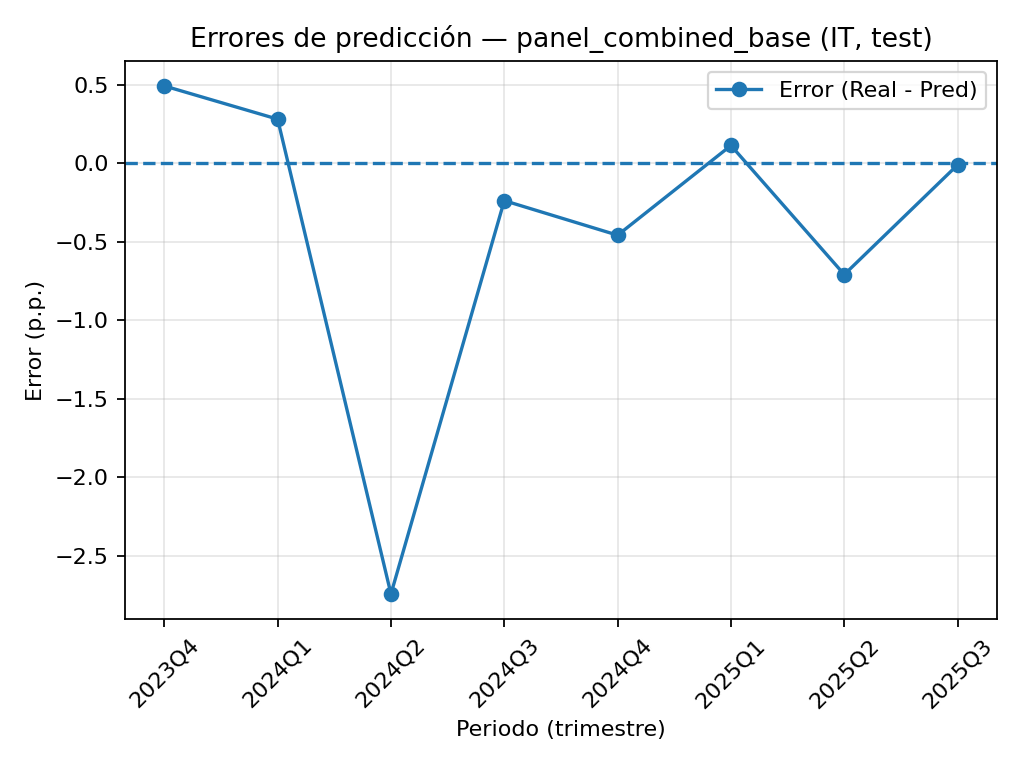
\includegraphics[width=\textwidth]{figures/bloque 1/panel_combined_base_it_errors.png}
    \caption{Errores de predicción -- panel combinado base (IT, test)}
    \label{fig:panel_base_it_err}
\end{minipage}\hfill
\begin{minipage}[t]{0.48\textwidth}
    \centering
    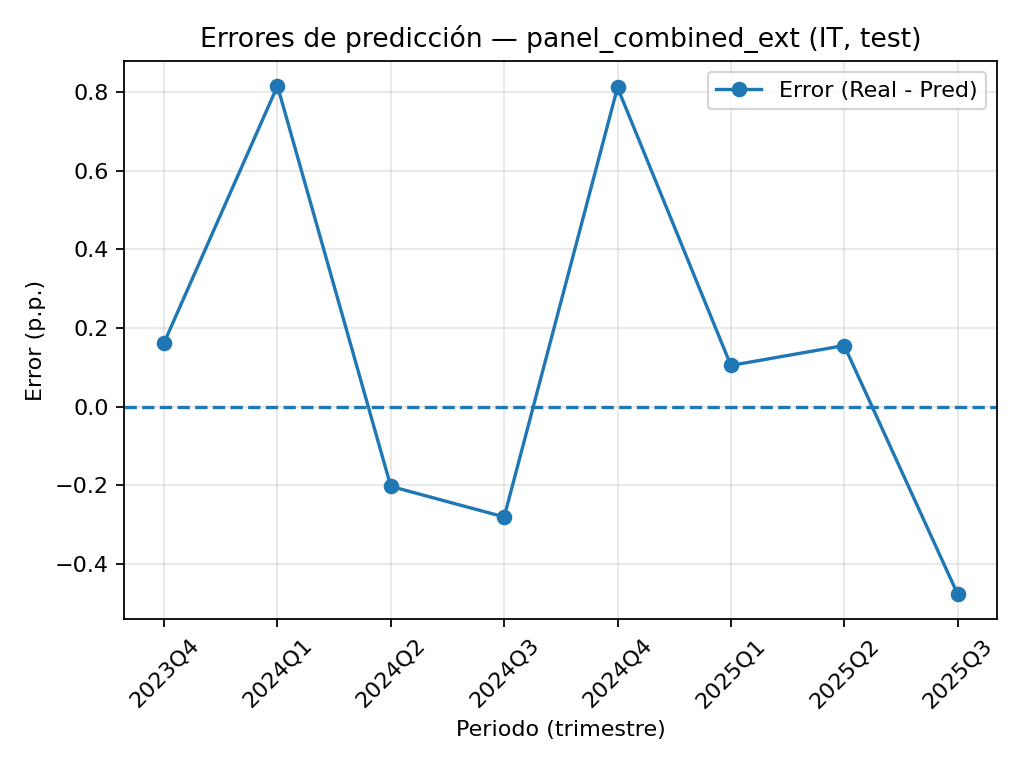
\includegraphics[width=\textwidth]{figures/bloque 1/panel_combined_ext_it_errors.png}
    \caption{Errores de predicción -- panel combinado ampliado (IT, test)}
    \label{fig:panel_ext_it_err}
\end{minipage}
\end{figure}

\FloatBarrier
\subsection{Importancia de variables}

Las Figuras~\ref{fig:panel_feat_base} y~\ref{fig:panel_feat_ext} muestran la importancia relativa de las variables en el modelo panel para las configuraciones base y ampliada respectivamente.

En el modelo base (Figura~\ref{fig:panel_feat_base}), las únicas dos variables disponibles ---inflación rezagada (\texttt{inflation\_\allowbreak{}qoq\_\allowbreak{}pct\_\allowbreak{}l1}) y tasa de desempleo rezagada (\texttt{unemployment\_\allowbreak{}rate\_\allowbreak{}l1})--- presentan una importancia relativamente equilibrada, con la inflación algo por encima (ganancia aproximada de 6.3 frente a 4.1). Este reparto contrasta con la dominancia habitual de los retardos del PIB en el modelo ampliado, y sugiere que, cuando no se dispone de información autorregresiva, ambos indicadores macroeconómicos aportan señal útil de forma complementaria.

En el modelo ampliado (Figura~\ref{fig:panel_feat_ext}), el retardo inmediato del PIB (\texttt{gdp\_\allowbreak{}qoq\_\allowbreak{}pct\_\allowbreak{}l1}) concentra de nuevo la mayor parte de la importancia explicativa (ganancia próxima a 15), reproduciendo el patrón ya observado en el Bloque~0 para los modelos por país. El índice de producción industrial (\texttt{ipi\_\allowbreak{}qoq\_\allowbreak{}pct\_\allowbreak{}l1}) y el comercio minorista (\texttt{retail\_\allowbreak{}qoq\_\allowbreak{}pct\_\allowbreak{}l1}) ocupan el segundo y tercer lugar respectivamente, con ganancias en torno a 2.5 y 2.0. El desempleo y la inflación rezagados mantienen una contribución marginal, lo que confirma que, una vez disponibles los retardos del PIB y los indicadores de actividad, las variables de mercado laboral y precios no añaden capacidad predictiva adicional a un horizonte de un trimestre.

\begin{figure}[H]
\centering
\begin{minipage}[t]{0.48\textwidth}
    \centering
    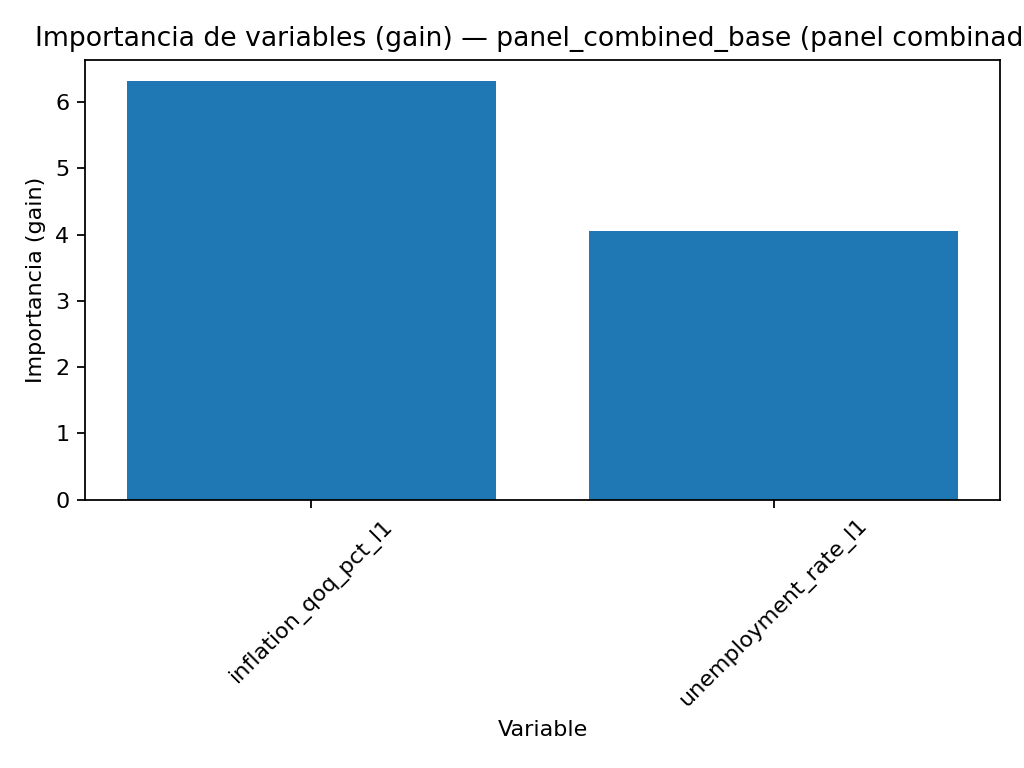
\includegraphics[width=\textwidth]{figures/bloque 1/panel_combined_base_combined_feature_importance.png}
    \caption{Importancia de variables (gain) -- panel combinado base}
    \label{fig:panel_feat_base}
\end{minipage}\hfill
\begin{minipage}[t]{0.48\textwidth}
    \centering
    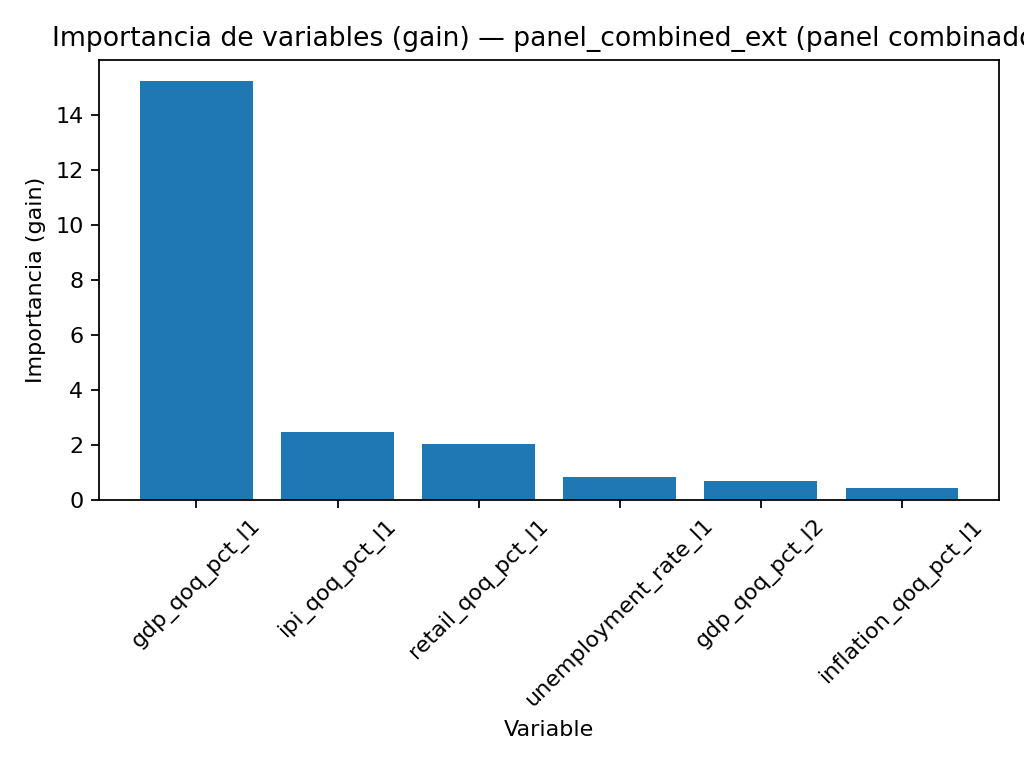
\includegraphics[width=\textwidth]{figures/bloque 1/panel_combined_ext_combined_feature_importance.png}
    \caption{Importancia de variables (gain) -- panel combinado ampliado}
    \label{fig:panel_feat_ext}
\end{minipage}
\end{figure}

\FloatBarrier
\subsection{Síntesis del Bloque 1}

El entrenamiento con datos combinados de los tres países produce mejoras generalizadas respecto al Bloque~0, siendo el efecto más significativo la rehabilitación del modelo ampliado para España, que pasa de ser el peor resultado individual (MAE 0.796) al mejor del bloque (MAE 0.297). Este resultado sugiere que el sobreajuste observado en el Bloque~0 podría estar relacionado principalmente con la escasez de datos de entrenamiento, más que con una limitación inherente de las variables seleccionadas.

Desde una perspectiva metodológica, el modelo panel ampliado se consolida como la configuración más robusta del bloque: obtiene el mejor MAE en los tres países de forma simultánea, algo que ninguna configuración del Bloque~0 lograba. La tabla comparativa entre bloques ilustra esta consistencia: frente a la heterogeneidad de resultados del Bloque~0 ---donde la configuración óptima variaba según el país---, el modelo panel ampliado ofrece un resultado competitivo de forma uniforme.

Italia sigue siendo el país más difícil de predecir, con un MAE del modelo ampliado (0.376) que duplica aproximadamente el de España (0.297) y supera al de Francia (0.215). Esto apunta a que la economía italiana presenta una dinámica trimestral menos persistente o más sensible a factores no capturados por las variables del panel, lo que motiva la exploración de enfoques que permitan al modelo distinguir explícitamente entre economías, abordada en el Bloque~2.

% ══════════════════════════════════════════════════════════════════════
\FloatBarrier
\section{Bloque 2 --- Panel con variable \emph{geo} como feature}

\textbf{Idea principal:} incorporar dummies de país resulta beneficioso únicamente cuando el modelo ya dispone de variables autorregresivas. Sin ellas, las dummies parecen sobreexplotarse y degradan gravemente las predicciones ---con un colapso extremo en Italia (MAE 4.324)---. El modelo ampliado con geo obtiene resultados similares o ligeramente superiores a los del Bloque~1.

El tercer bloque de experimentos parte de la misma arquitectura del Bloque~1 pero introduce
una modificación conceptualmente relevante: la variable de país se incorpora explícitamente
como feature mediante codificación \emph{one-hot}, añadiendo tres columnas binarias
(\texttt{geo\_ES}, \texttt{geo\_FR}, \texttt{geo\_IT}) al vector de entrada del modelo.

En el Bloque~1, el modelo panel compartía todos sus parámetros sin distinguir la procedencia
de cada observación; el único mecanismo de diferenciación era indirecto, a través de las
diferencias en los valores de los indicadores macroeconómicos entre países. El Bloque~2
permite que el modelo aprenda umbrales y reglas distintos para cada economía sin necesidad
de entrenar modelos separados.

El dataset, la partición temporal, los hiperparámetros del modelo XGBoost y las dos
configuraciones de features (base y ampliada) son idénticos a los bloques anteriores.
La única diferencia es la adición de \texttt{geo\_ES}, \texttt{geo\_FR} y \texttt{geo\_IT}
al final del vector de entrada en ambas configuraciones, elevando el número de features
de 2 a 5 en el modelo base, y de 6 a 9 en el modelo ampliado.

Los resultados obtenidos en el conjunto de prueba para los tres países son los siguientes:

\begin{table}[H]
\centering
\caption{Comparativa de modelos panel con geo como feature por país -- Bloque 2}
\label{tab:bloque2}
\small
\begin{tabular}{lcccccc}
\hline
 & \multicolumn{2}{c}{\textbf{España}} & \multicolumn{2}{c}{\textbf{Francia}} & \multicolumn{2}{c}{\textbf{Italia}} \\
\textbf{Modelo} & \textbf{MAE} & \textbf{RMSE} & \textbf{MAE} & \textbf{RMSE} & \textbf{MAE} & \textbf{RMSE} \\
\hline
panel\_geo\_base & 0.423 & 0.466 & 0.819 & 1.021 & 4.324 & 6.518 \\
panel\_geo\_ext  & 0.290 & 0.331 & 0.224 & 0.270 & 0.365 & 0.451 \\
\hline
\end{tabular}
\end{table}

El contraste entre ambas configuraciones es el más acusado de todos los bloques analizados:
el modelo base con dummies de país registra resultados muy inferiores a los del Bloque~1,
mientras que el modelo ampliado mantiene o mejora marginalmente los resultados previos.

\FloatBarrier
\subsection{España}

Para España, el modelo base del panel geo obtiene un MAE de 0.423, superior a los 0.363 del
Bloque~1. Como muestra la Figura~\ref{fig:b2_base_es_pred}, el modelo subestima de forma
sistemática el crecimiento en los primeros trimestres del horizonte de prueba y sobreestima
bruscamente en 2024Q3, para finalmente caer a territorio negativo en 2025Q3 cuando la
economía española aún crecía 0.64~p.p. El gráfico de errores
(Figura~\ref{fig:b2_base_es_err}) refleja esta inestabilidad con una alternancia de signo
pronunciada que supera los $\pm$0.6~p.p. en varios trimestres.

El modelo ampliado obtiene un MAE de 0.290, su mejor resultado en todos los bloques para
España, con una mejora marginal respecto a los 0.297 del Bloque~1. La
Figura~\ref{fig:b2_ext_es_pred} muestra que las dos curvas evolucionan de forma muy similar,
sin llegar a producir ninguna predicción anómala. El gráfico de errores
(Figura~\ref{fig:b2_ext_es_err}) no presenta sesgo sistemático, con valores que oscilan
entre $-$0.29 y 0.55~p.p.

\begin{figure}[H]
\centering
\begin{minipage}[t]{0.48\textwidth}
    \centering
    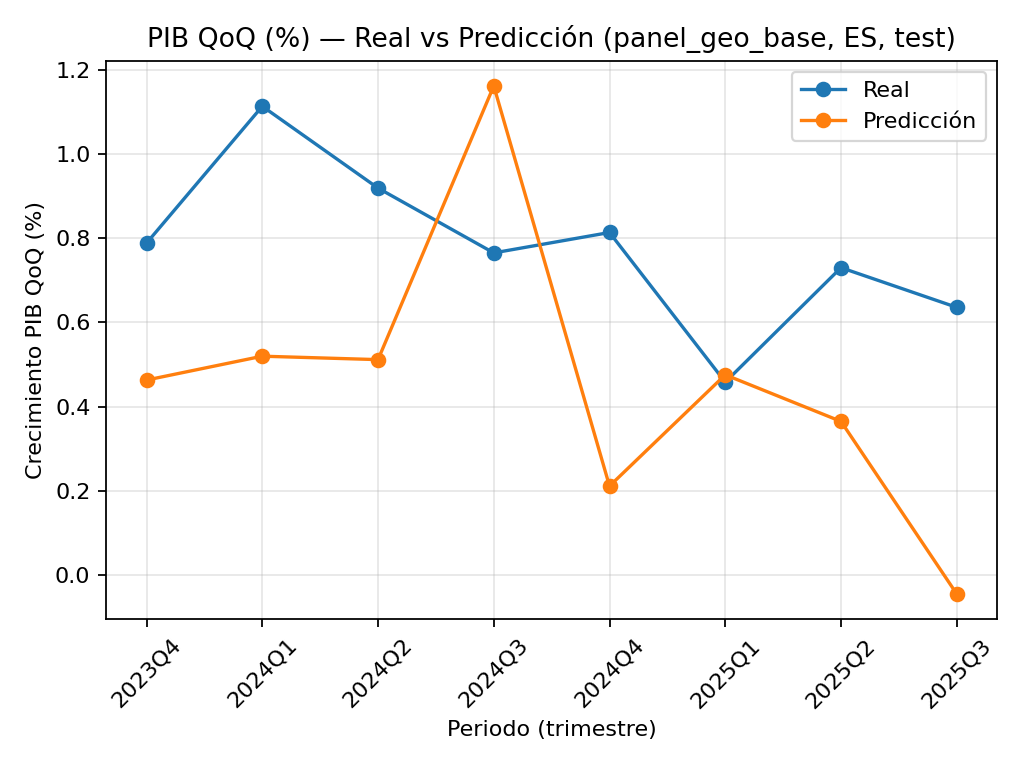
\includegraphics[width=\textwidth]{figures/bloque 2/panel_geo_base_es_real_vs_pred.png}
    \caption{PIB QoQ real vs predicción -- panel geo base (ES, test)}
    \label{fig:b2_base_es_pred}
\end{minipage}\hfill
\begin{minipage}[t]{0.48\textwidth}
    \centering
    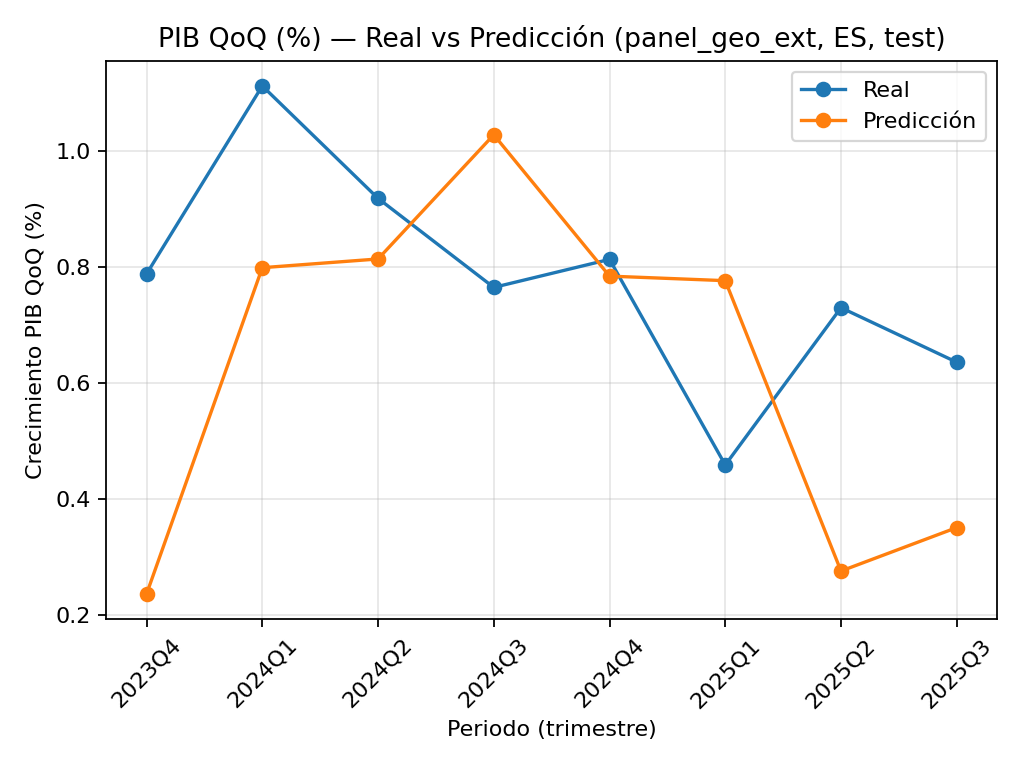
\includegraphics[width=\textwidth]{figures/bloque 2/panel_geo_ext_es_real_vs_pred.png}
    \caption{PIB QoQ real vs predicción -- panel geo ampliado (ES, test)}
    \label{fig:b2_ext_es_pred}
\end{minipage}

\vspace{0.5em}

\begin{minipage}[t]{0.48\textwidth}
    \centering
    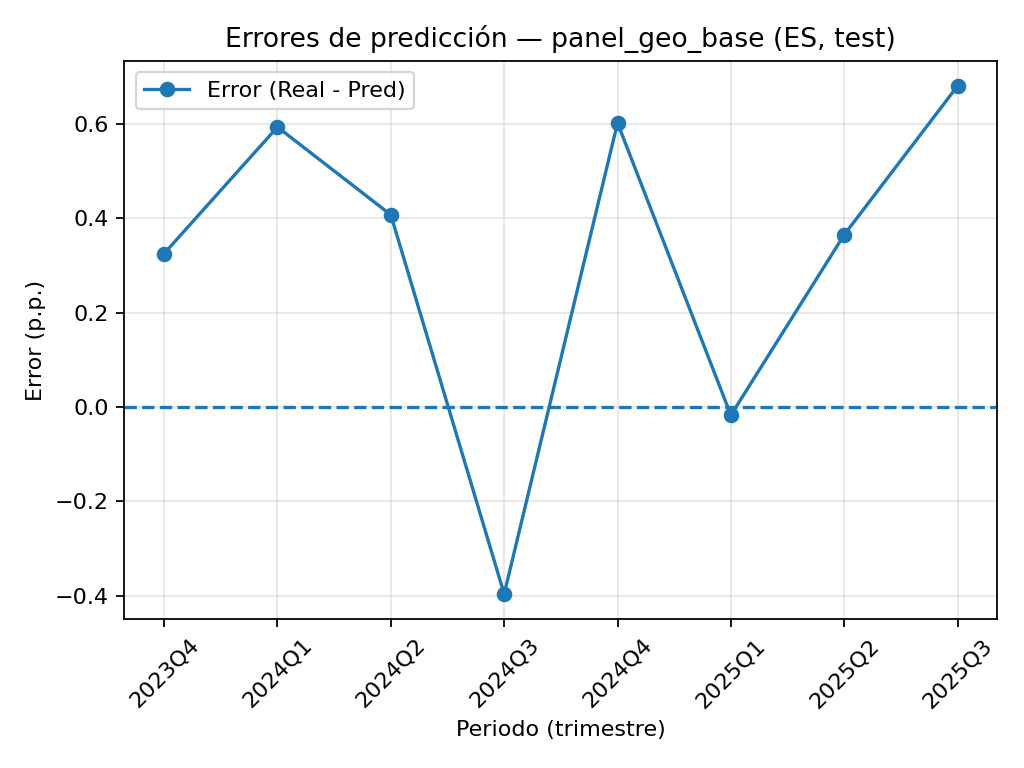
\includegraphics[width=\textwidth]{figures/bloque 2/panel_geo_base_es_errors.png}
    \caption{Errores de predicción -- panel geo base (ES, test)}
    \label{fig:b2_base_es_err}
\end{minipage}\hfill
\begin{minipage}[t]{0.48\textwidth}
    \centering
    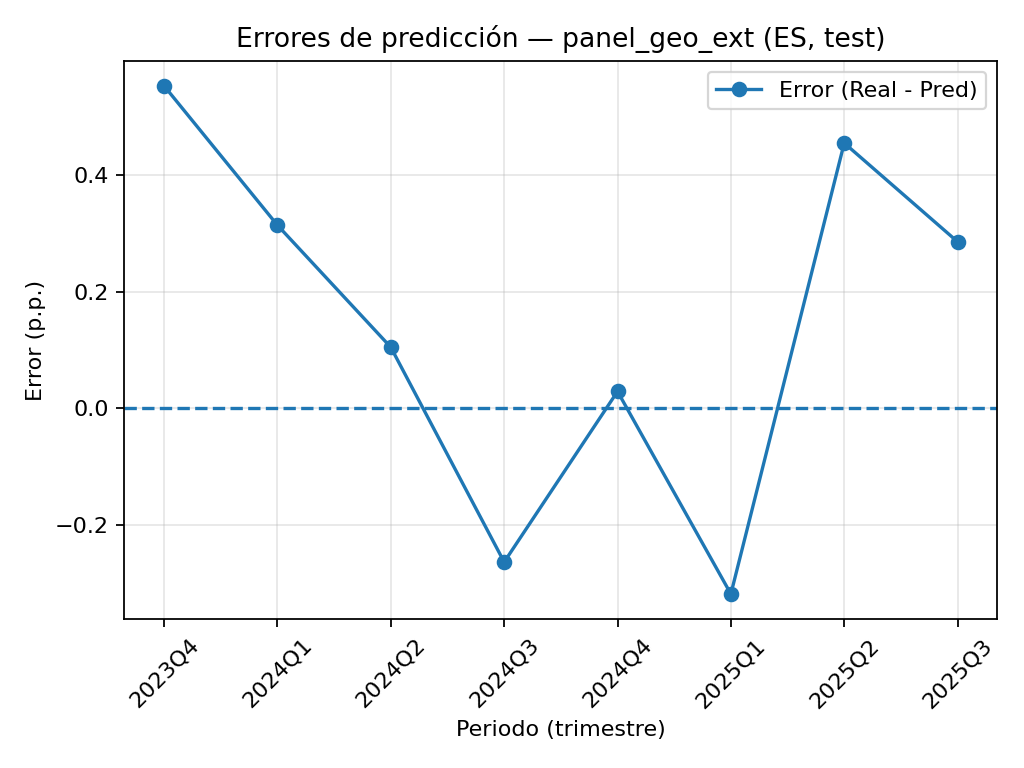
\includegraphics[width=\textwidth]{figures/bloque 2/panel_geo_ext_es_errors.png}
    \caption{Errores de predicción -- panel geo ampliado (ES, test)}
    \label{fig:b2_ext_es_err}
\end{minipage}
\end{figure}

\FloatBarrier
\subsection{Francia}

Francia es el país donde la introducción de las dummies de país produce el deterioro más
severo en la configuración base, pasando de un MAE de 0.316 en el Bloque~1 a 0.819 en el
Bloque~2. La Figura~\ref{fig:b2_base_fr_pred} ilustra el problema de forma inequívoca:
mientras que el crecimiento real de Francia se mantiene en un rango estrecho a lo largo del
periodo de prueba, las predicciones oscilan violentamente, con errores que alcanzan valores
inferiores a $-$1.5~p.p. en varios trimestres de 2025
(Figura~\ref{fig:b2_base_fr_err}). Este comportamiento se explica porque, sin los retardos
del PIB que anclen las predicciones al nivel de actividad reciente, la dummy
\texttt{geo\_FR} lleva al modelo a activar regiones del espacio de features asociadas en el
entrenamiento a trimestres de alto crecimiento francés que no vuelven a reproducirse en el
periodo de prueba.

El modelo ampliado recupera la capacidad predictiva con un MAE de 0.224, apenas
0.009~p.p. superior al 0.215 del Bloque~1, diferencia que se sitúa dentro de la variabilidad
esperada con solo 8 observaciones de prueba. La Figura~\ref{fig:b2_ext_fr_pred} muestra que
la predicción sigue la evolución real con razonable fidelidad, con errores contenidos en la
mayor parte del periodo (Figura~\ref{fig:b2_ext_fr_err}).

\begin{figure}[H]
\centering
\begin{minipage}[t]{0.48\textwidth}
    \centering
    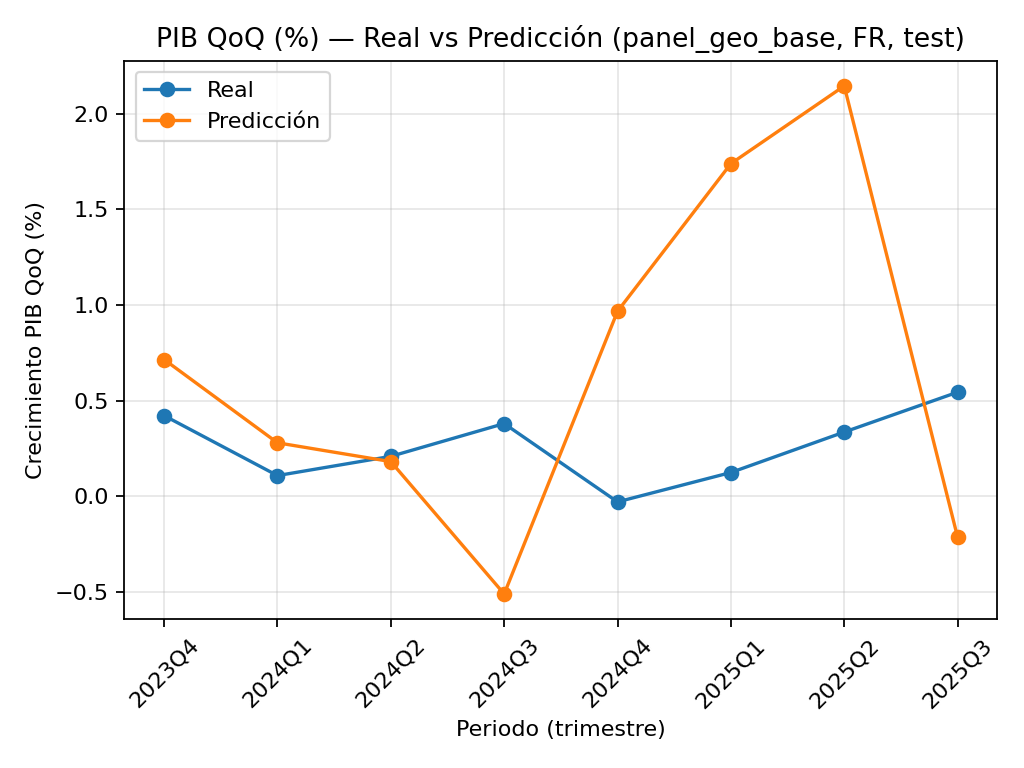
\includegraphics[width=\textwidth]{figures/bloque 2/panel_geo_base_fr_real_vs_pred.png}
    \caption{PIB QoQ real vs predicción -- panel geo base (FR, test)}
    \label{fig:b2_base_fr_pred}
\end{minipage}\hfill
\begin{minipage}[t]{0.48\textwidth}
    \centering
    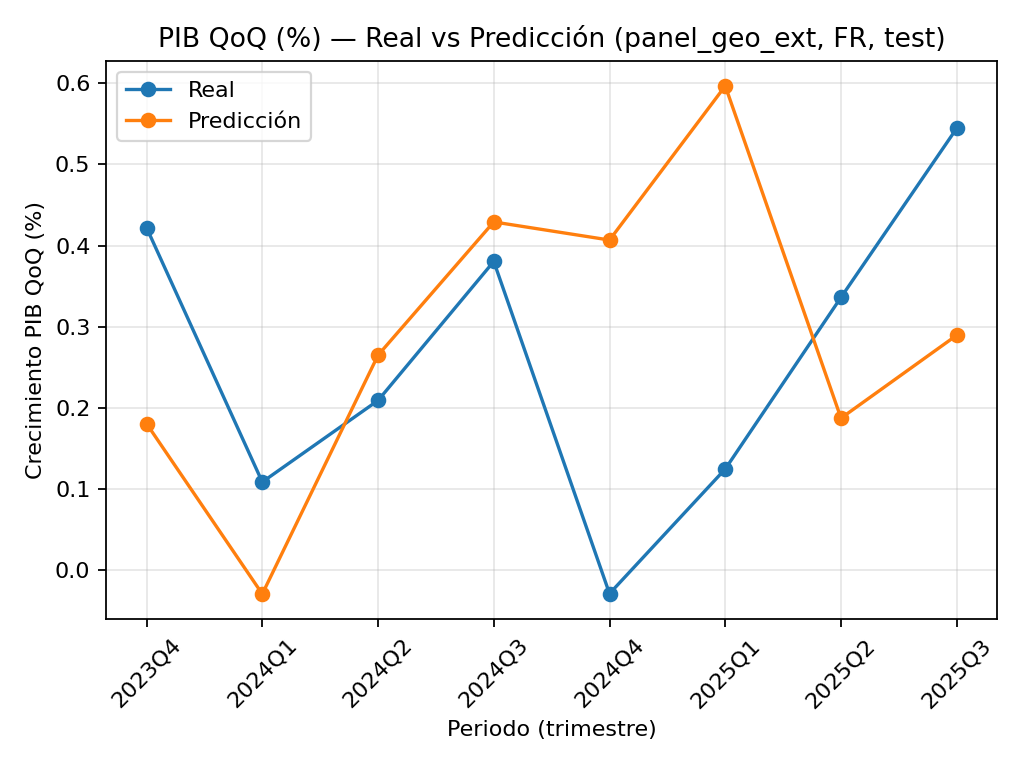
\includegraphics[width=\textwidth]{figures/bloque 2/panel_geo_ext_fr_real_vs_pred.png}
    \caption{PIB QoQ real vs predicción -- panel geo ampliado (FR, test)}
    \label{fig:b2_ext_fr_pred}
\end{minipage}

\vspace{0.5em}

\begin{minipage}[t]{0.48\textwidth}
    \centering
    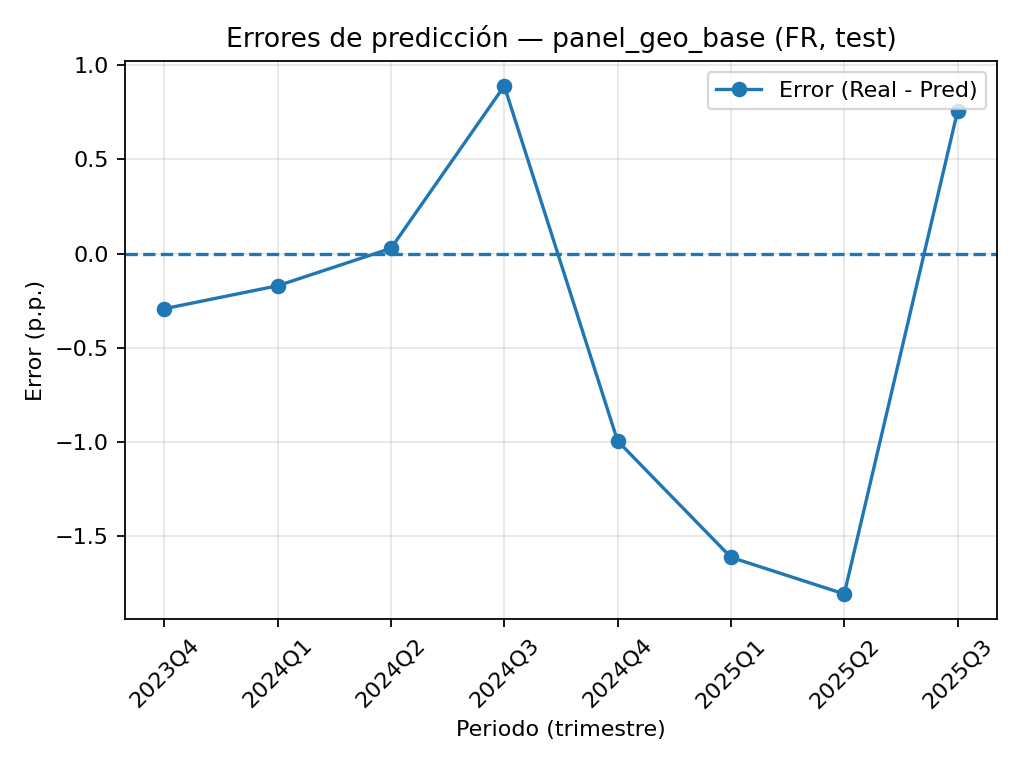
\includegraphics[width=\textwidth]{figures/bloque 2/panel_geo_base_fr_errors.png}
    \caption{Errores de predicción -- panel geo base (FR, test)}
    \label{fig:b2_base_fr_err}
\end{minipage}\hfill
\begin{minipage}[t]{0.48\textwidth}
    \centering
    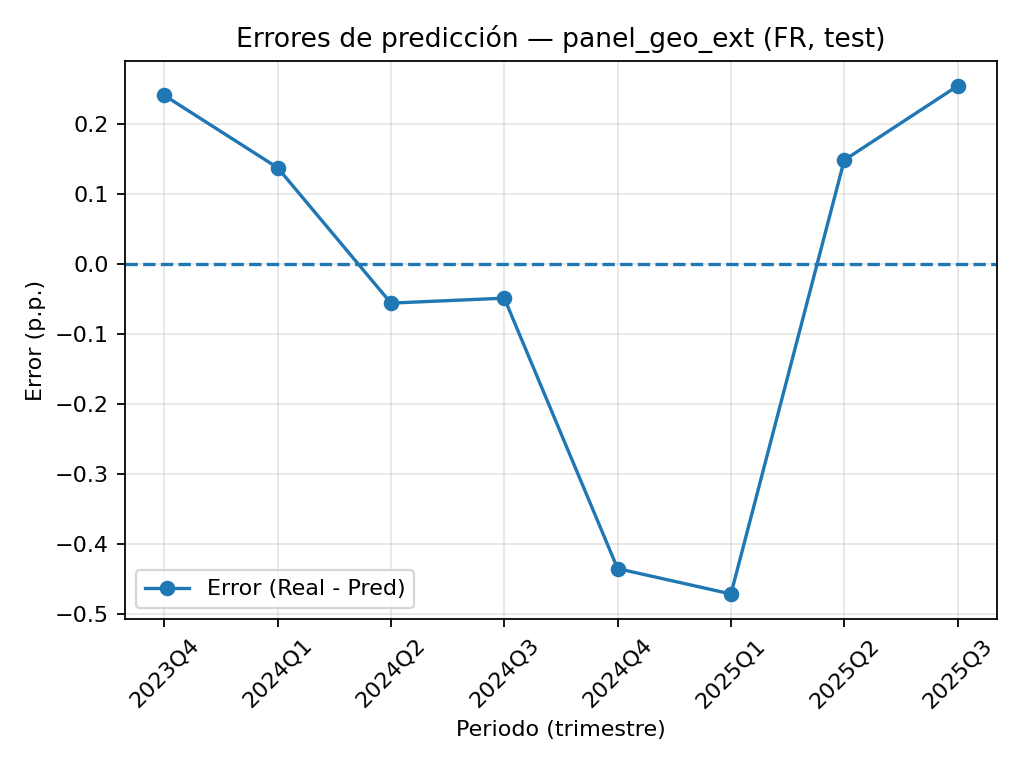
\includegraphics[width=\textwidth]{figures/bloque 2/panel_geo_ext_fr_errors.png}
    \caption{Errores de predicción -- panel geo ampliado (FR, test)}
    \label{fig:b2_ext_fr_err}
\end{minipage}
\end{figure}

\FloatBarrier
\subsection{Italia}

Italia registra el resultado más extremo de todos los experimentos realizados: el modelo base
con dummies de país obtiene un MAE de 4.324 y un RMSE de 6.518, frente a los 0.631 y 1.039
del Bloque~1. La Figura~\ref{fig:b2_base_it_pred} muestra predicciones completamente
desconectadas de la realidad, con valores que alcanzan magnitudes imposibles en el contexto
del crecimiento trimestral. La causa reside en la interacción entre la dummy
\texttt{geo\_IT} y la ausencia de variables autorregresivas: durante el entrenamiento, el
modelo aprende que la combinación de valores bajos de desempleo e inflación rezagados junto
con \texttt{geo\_IT}=1 se corresponde, en algunos trimestres de la recuperación
2020--2022, con crecimientos muy elevados del PIB. Al llegar al periodo de prueba, el modelo
aplica esa regla aprendida fuera del contexto económico que la originó, produciendo
predicciones que ilustran un caso clásico de sobreajuste catastrófico por sobreexplotación
de la señal de identidad categórica.

El modelo ampliado corrige completamente este comportamiento, obteniendo un MAE de 0.365
y un RMSE de 0.451, que supera incluso al modelo ampliado del Bloque~1 (MAE 0.376, RMSE
0.466). La Figura~\ref{fig:b2_ext_it_pred} muestra que el modelo sigue razonablemente la
dirección general del crecimiento italiano, aunque con errores de amplitud en los trimestres
2024Q1 y 2024Q4, donde no anticipa la moderación de la actividad económica. Este patrón,
ya observado en bloques anteriores, apunta a que la dinámica italiana presenta quiebros de
dirección que los retardos del PIB no logran anticipar de forma sistemática.

\begin{figure}[H]
\centering
\begin{minipage}[t]{0.48\textwidth}
    \centering
    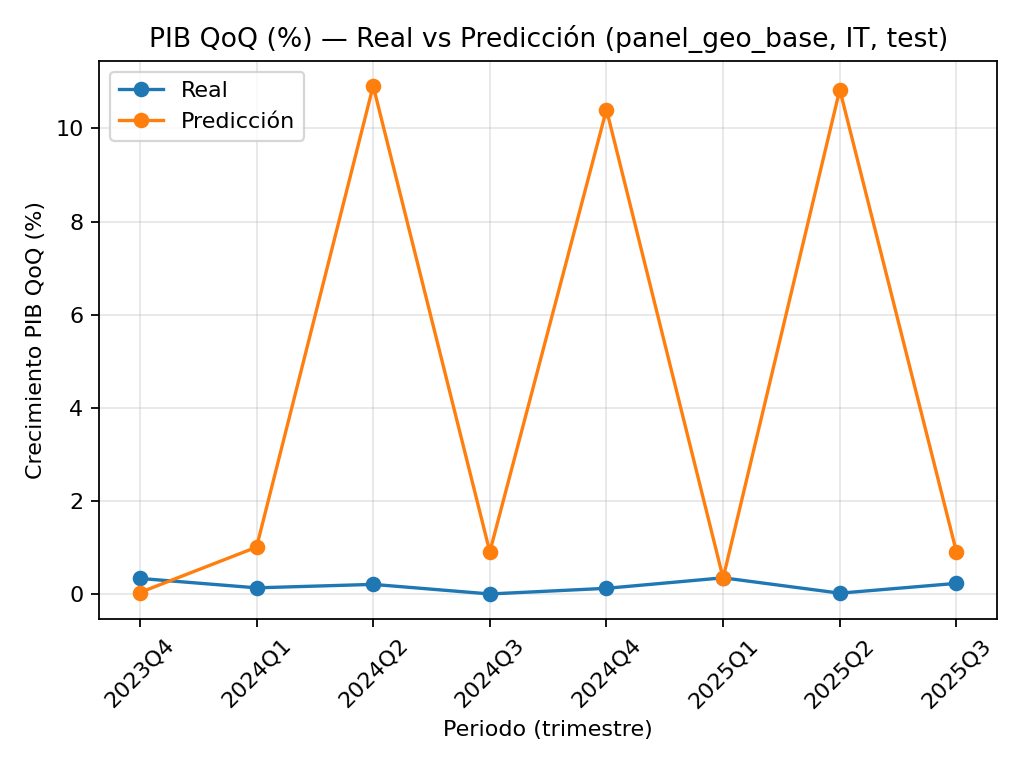
\includegraphics[width=\textwidth]{figures/bloque 2/panel_geo_base_it_real_vs_pred.png}
    \caption{PIB QoQ real vs predicción -- panel geo base (IT, test)}
    \label{fig:b2_base_it_pred}
\end{minipage}\hfill
\begin{minipage}[t]{0.48\textwidth}
    \centering
    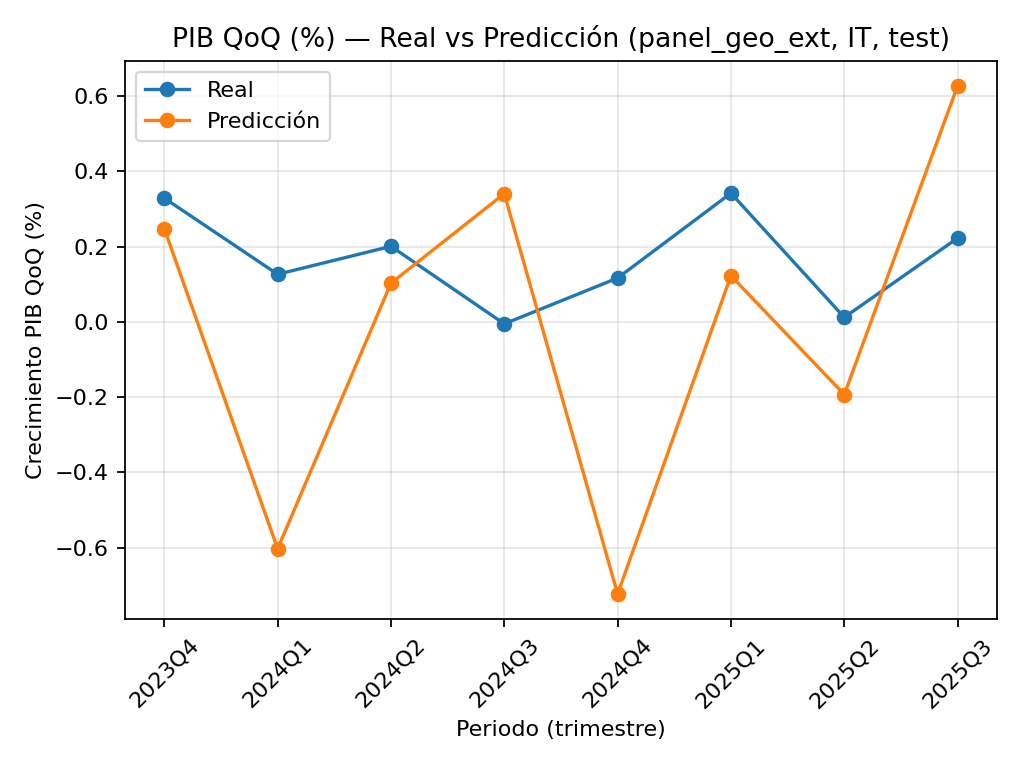
\includegraphics[width=\textwidth]{figures/bloque 2/panel_geo_ext_it_real_vs_pred.png}
    \caption{PIB QoQ real vs predicción -- panel geo ampliado (IT, test)}
    \label{fig:b2_ext_it_pred}
\end{minipage}

\vspace{0.5em}

\begin{minipage}[t]{0.48\textwidth}
    \centering
    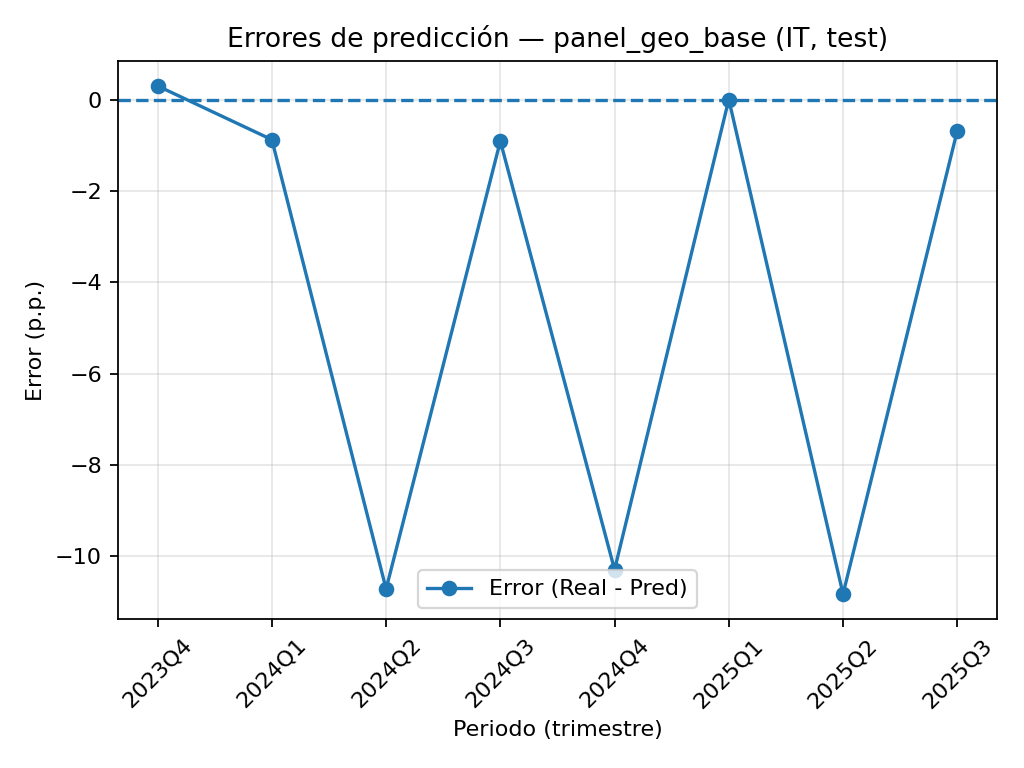
\includegraphics[width=\textwidth]{figures/bloque 2/panel_geo_base_it_errors.png}
    \caption{Errores de predicción -- panel geo base (IT, test)}
    \label{fig:b2_base_it_err}
\end{minipage}\hfill
\begin{minipage}[t]{0.48\textwidth}
    \centering
    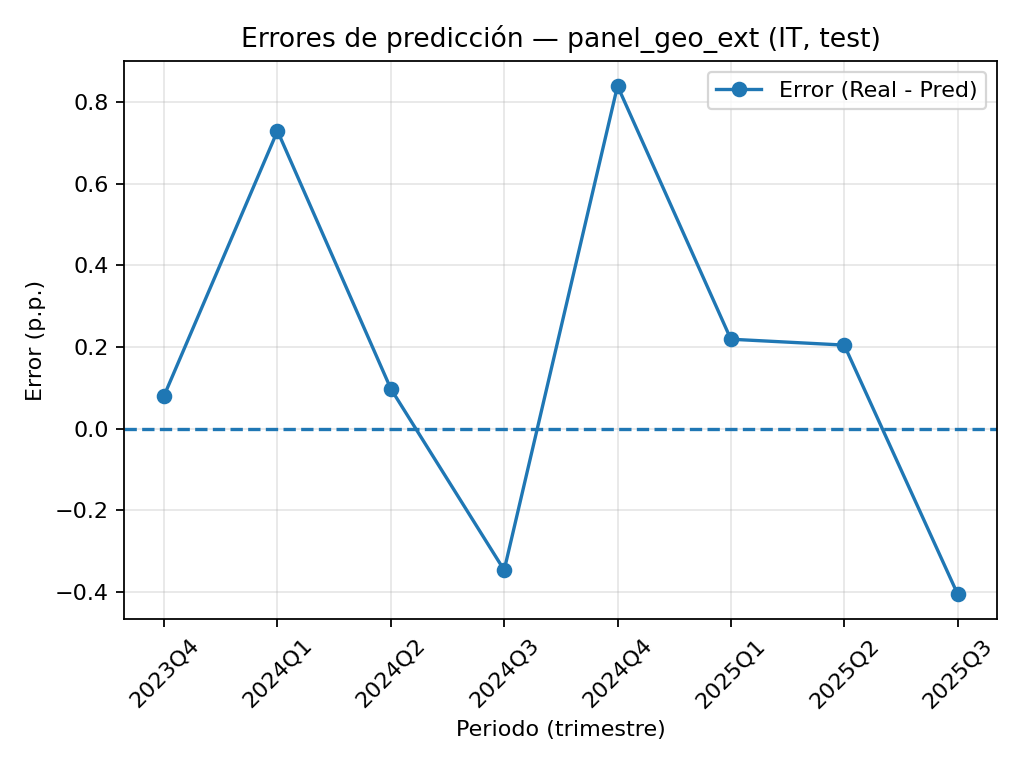
\includegraphics[width=\textwidth]{figures/bloque 2/panel_geo_ext_it_errors.png}
    \caption{Errores de predicción -- panel geo ampliado (IT, test)}
    \label{fig:b2_ext_it_err}
\end{minipage}
\end{figure}

\FloatBarrier
\subsection{Importancia de variables}

Las Figuras~\ref{fig:b2_base_imp} y~\ref{fig:b2_ext_imp} muestran la importancia relativa
de las variables en el modelo panel geo para las configuraciones base y ampliada respectivamente.

En el modelo base (Figura~\ref{fig:b2_base_imp}), las variables económicas
\texttt{unemployment\_\allowbreak{}rate\_\allowbreak{}l1} e \texttt{inflation\_\allowbreak{}qoq\_\allowbreak{}pct\_\allowbreak{}l1} siguen ocupando los
primeros puestos, tal y como ocurría en el Bloque~1. Sin embargo, la novedad más reveladora
es que \texttt{geo\_FR} ocupa el tercer lugar con una ganancia notablemente superior a la de
\texttt{geo\_ES} y \texttt{geo\_IT}. Esta jerarquía explica directamente el deterioro de
las predicciones francesas: el modelo dedica una fracción significativa de su capacidad de
división a identificar si la observación pertenece a Francia, asociando esa identidad a un
nivel de crecimiento elevado que no se corresponde con el periodo de prueba.

En el modelo ampliado (Figura~\ref{fig:b2_ext_imp}), el retardo inmediato del PIB
(\texttt{gdp\_\allowbreak{}qoq\_\allowbreak{}pct\_\allowbreak{}l1}) concentra de nuevo la mayor parte de la importancia
explicativa, reproduciendo el patrón dominante ya observado en los Bloques~0 y~1. El
resultado más importante desde la perspectiva de este bloque es que las tres dummies de
país presentan ganancias marginales, inferiores a 0.3 frente a las $\approx$16 unidades del
retardo del PIB. Una vez disponibles los retardos del PIB y los indicadores de actividad,
el modelo prácticamente ignora la información de identidad nacional, lo que sugiere que la
información geográfica podría estar ya codificada de forma implícita en la dinámica autorregresiva
de cada economía.

\begin{figure}[H]
\centering
\begin{minipage}[t]{0.48\textwidth}
    \centering
    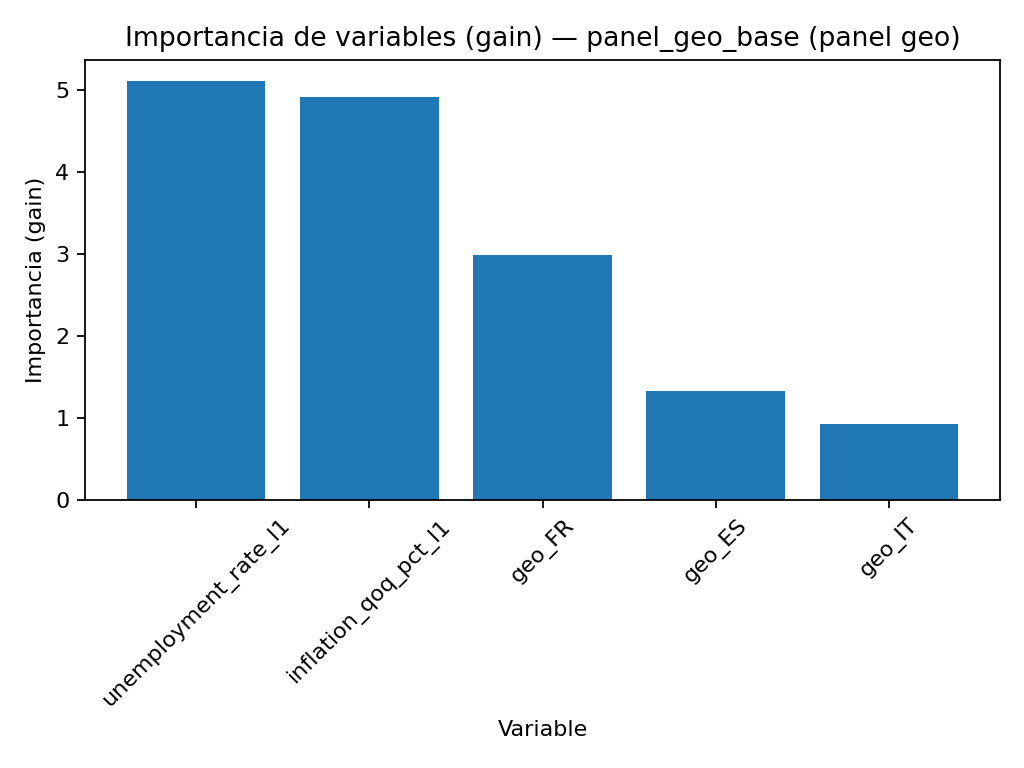
\includegraphics[width=\textwidth]{figures/bloque 2/panel_geo_base_combined_feature_importance.png}
    \caption{Importancia de variables (gain) -- panel geo base}
    \label{fig:b2_base_imp}
\end{minipage}\hfill
\begin{minipage}[t]{0.48\textwidth}
    \centering
    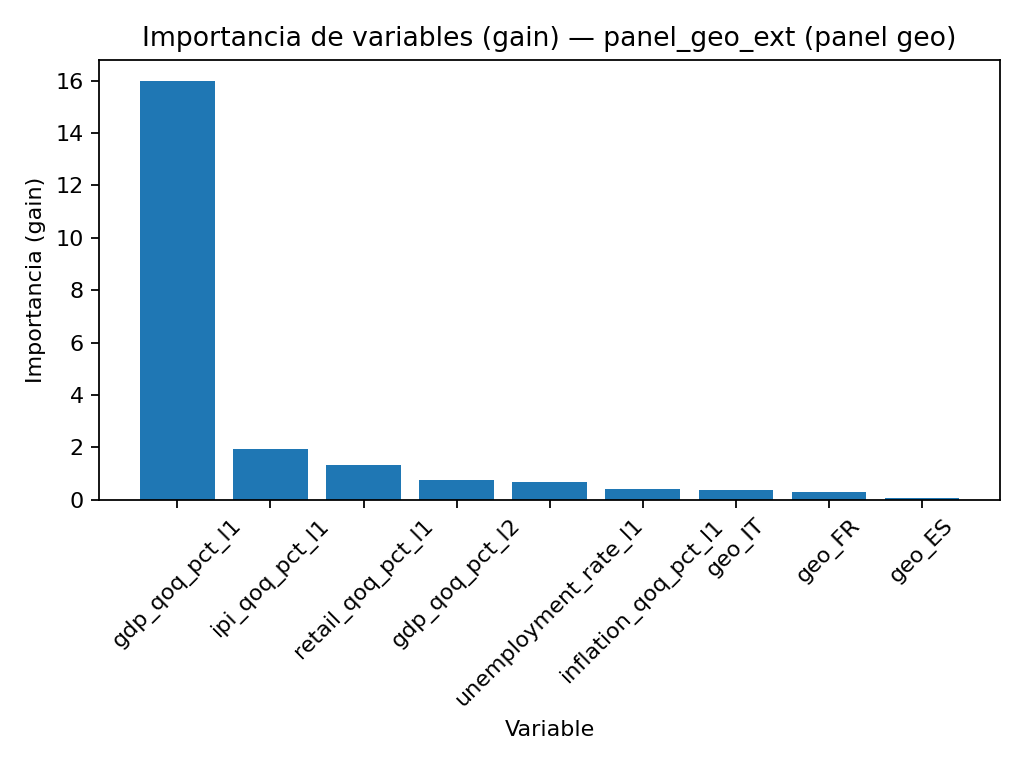
\includegraphics[width=\textwidth]{figures/bloque 2/panel_geo_ext_combined_feature_importance.png}
    \caption{Importancia de variables (gain) -- panel geo ampliado}
    \label{fig:b2_ext_imp}
\end{minipage}
\end{figure}

\FloatBarrier
\subsection{Síntesis del Bloque 2}

Los resultados del Bloque~2 revelan que la codificación de la variable de país como feature
es un arma de doble filo cuya eficacia depende críticamente de las variables económicas
disponibles en el modelo.

Cuando el modelo cuenta con los retardos del PIB y los indicadores de actividad
---configuración ampliada---, las dummies de país no aportan capacidad predictiva adicional
apreciable pero tampoco perjudican: los resultados son prácticamente idénticos a los del
Bloque~1 o ligeramente superiores en España e Italia. En este escenario, la identidad
geográfica queda subsumida por la información autorregresiva, que ya codifica de forma
implícita las diferencias de nivel y volatilidad entre economías.

En cambio, cuando el modelo base carece de esa información de anclaje, las dummies de
país se convierten en la señal más distintiva disponible y el modelo las sobreexplota. El
resultado es una regresión hacia medias de entrenamiento específicas de cada país que ya no
son representativas del periodo de prueba, con un deterioro especialmente grave en Francia
y un colapso catastrófico en Italia (MAE 4.324 frente a 0.631 en el Bloque~1).

Desde una perspectiva metodológica, este experimento apunta a que las variables de
identidad categórica ---país, sector, empresa--- en modelos de series temporales
macroeconómicas podrían ser secundarias respecto a las variables de estado autorregresivas. El nivel
reciente de actividad económica es un predictor mucho más informativo que la etiqueta del
país al que pertenece la observación, y ningún mecanismo de codificación categórica puede
sustituir esa información cuando no está disponible.

El modelo ampliado del Bloque~2 (\texttt{panel\_geo\_ext}) obtiene el mejor MAE para
España (0.290) y para Italia (0.365) de todos los bloques hasta este punto, y un resultado
prácticamente idéntico al Bloque~1 en Francia (0.224 frente a 0.215). Estos resultados
motivan la exploración del Bloque~3, donde se analiza la capacidad de transferencia entre
economías entrenando con los datos de dos países y evaluando sobre el tercero.

% ══════════════════════════════════════════════════════════════════════
\FloatBarrier
\section{Bloque 3 --- Transferencia entre países}

\textbf{Idea principal:} entrenar con dos países y evaluar en un tercero que no ha
participado en el entrenamiento produce resultados sorprendentemente competitivos,
sugiriendo que los patrones macroeconómicos del ciclo trimestral son parcialmente
transferibles entre las economías analizadas.

En los bloques anteriores el país de evaluación siempre había aportado datos al
entrenamiento. El Bloque~3 rompe esta condición: se entrena un modelo XGBoost con la
configuración ampliada usando los datos de dos países y se evalúa sobre el tercero, que
no ha sido visto en ninguna fase del ajuste del modelo. Este diseño permite explorar si
los patrones macroeconómicos aprendidos de dos economías son lo suficientemente generales
como para generalizar a una tercera.

Se ejecutan las tres combinaciones posibles:

\begin{itemize}
    \item \textbf{ES + FR → IT}: entrena con España y Francia, evalúa en Italia.
    \item \textbf{ES + IT → FR}: entrena con España e Italia, evalúa en Francia.
    \item \textbf{FR + IT → ES}: entrena con Francia e Italia, evalúa en España.
\end{itemize}

En todos los casos se utiliza la configuración de features ampliada
(\texttt{gdp\_qoq\_pct\_l1}, \texttt{gdp\_qoq\_pct\_l2}, \texttt{unemployment\_rate\_l1},
\texttt{inflation\_qoq\_pct\_l1}, \texttt{ipi\_qoq\_pct\_l1}, \texttt{retail\_qoq\_pct\_l1}),
la misma partición temporal y los mismos hiperparámetros XGBoost de los bloques anteriores.
La configuración base no se incluye en este bloque dado que su rendimiento sin variables
autorregresivas fue consistentemente inferior en todos los experimentos previos.

Los resultados obtenidos son los siguientes:

\begin{table}[H]
\centering
\caption{Resultados del Bloque 3 --- Transferencia entre países (modelo ampliado)}
\label{tab:bloque3}
\small
\begin{tabular}{llcc}
\hline
\textbf{Entrenado con} & \textbf{Evaluado en} & \textbf{MAE} & \textbf{RMSE} \\
\hline
ES + FR & Italia  & 0.311 & 0.344 \\
ES + IT & Francia & 0.220 & 0.362 \\
FR + IT & España  & 0.337 & 0.367 \\
\hline
\end{tabular}
\end{table}

Para contextualizar estos valores, la Tabla~\ref{tab:comparativa_final} recoge los
resultados del modelo ampliado en todos los bloques para los tres países.

\begin{table}[H]
\centering
\caption{Comparativa del modelo ampliado entre todos los bloques}
\label{tab:comparativa_final}
\small
\begin{tabular}{lcccccc}
\hline
 & \multicolumn{2}{c}{\textbf{España}} & \multicolumn{2}{c}{\textbf{Francia}} & \multicolumn{2}{c}{\textbf{Italia}} \\
\textbf{Bloque} & \textbf{MAE} & \textbf{RMSE} & \textbf{MAE} & \textbf{RMSE} & \textbf{MAE} & \textbf{RMSE} \\
\hline
B0 — Por país       & 0.796 & 1.285 & 0.193 & 0.208 & 0.344 & 0.455 \\
B1 — Panel combinado & 0.297 & 0.331 & 0.215 & 0.256 & 0.376 & 0.466 \\
B2 — Panel con geo  & 0.290 & 0.331 & 0.224 & 0.270 & 0.365 & 0.451 \\
B3 — Transferencia  & 0.337 & 0.367 & 0.220 & 0.362 & 0.311 & 0.344 \\
\hline
\end{tabular}
\end{table}

\FloatBarrier
\subsection{Italia (ES+FR → IT)}

Italia es el resultado más llamativo del bloque. El modelo entrenado exclusivamente con
datos de España y Francia obtiene un MAE de 0.311 sobre Italia, mejorando tanto el
resultado del Bloque~0 con datos italianos propios (MAE 0.344) como los de los Bloques~1
y~2 (0.376 y 0.365 respectivamente). Este resultado apunta a que los patrones del ciclo
económico trimestral de España y Francia capturan regularidades compartidas con Italia
que no quedaban bien representadas cuando el modelo disponía únicamente de las~58
observaciones italianas de entrenamiento.

La Figura~\ref{fig:b3_it_pred} muestra que el modelo sigue razonablemente la dirección
del crecimiento italiano, sin producir predicciones anómalas extremas como las observadas
en el modelo base del Bloque~2.

\begin{figure}[H]
\centering
\begin{minipage}[t]{0.48\textwidth}
    \centering
    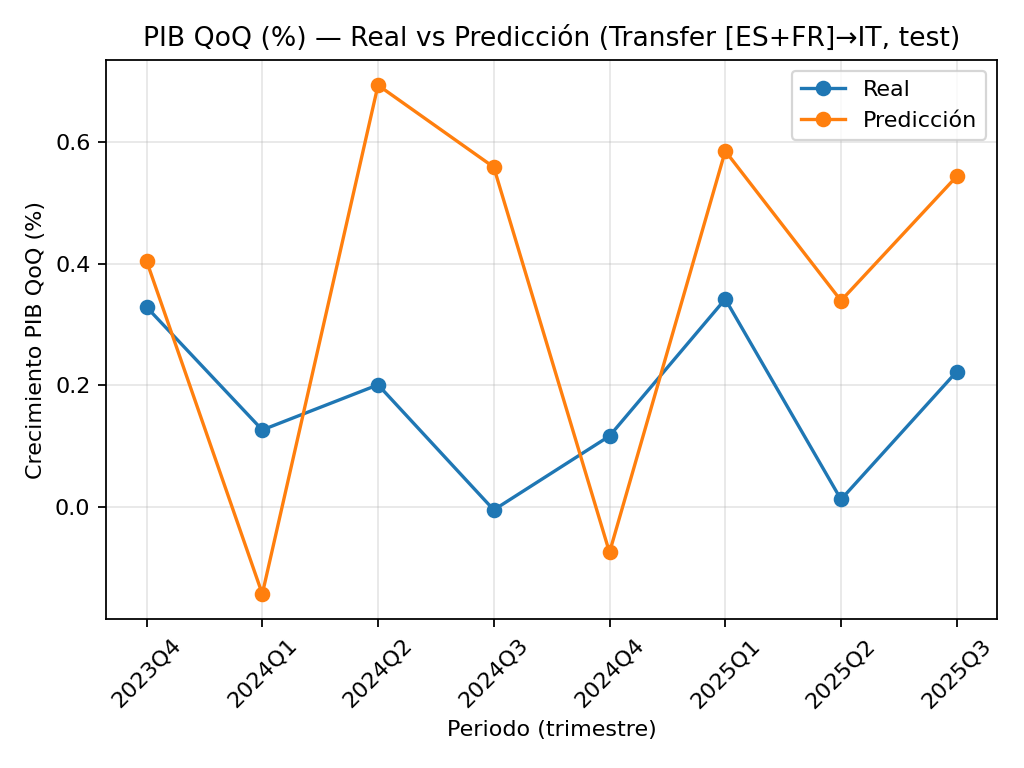
\includegraphics[width=\textwidth]{figures/bloque 3/panel_transfer_ext_it_real_vs_pred.png}
    \caption{PIB QoQ real vs predicción -- Transfer ES+FR → IT (test)}
    \label{fig:b3_it_pred}
\end{minipage}\hfill
\begin{minipage}[t]{0.48\textwidth}
    \centering
    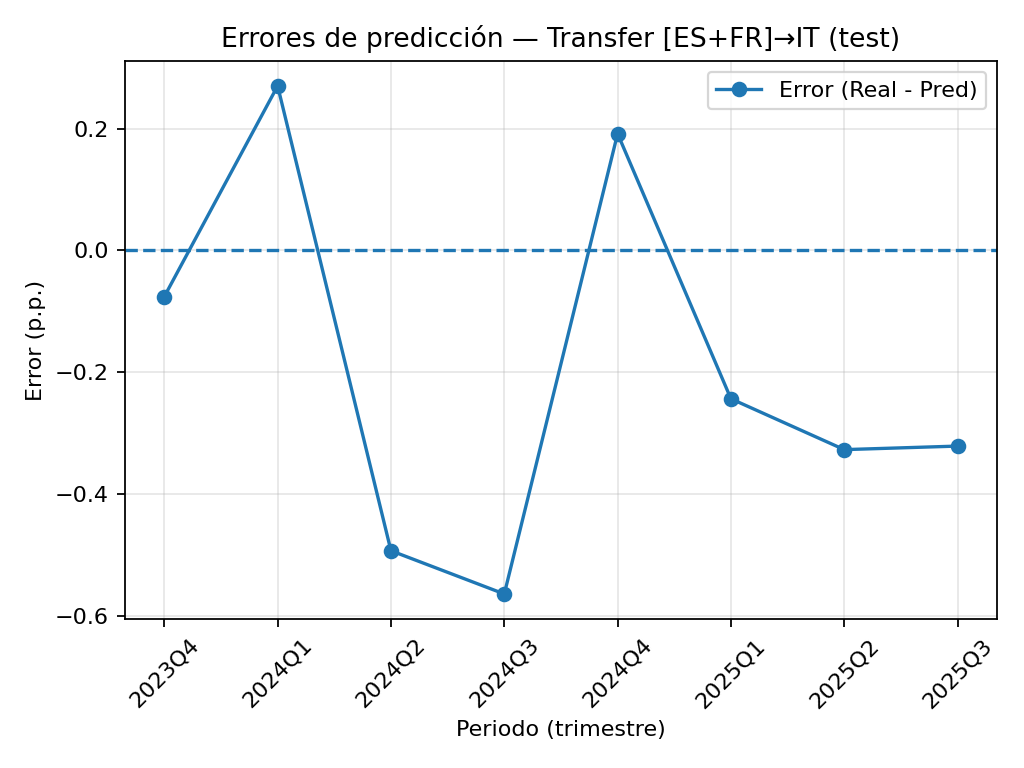
\includegraphics[width=\textwidth]{figures/bloque 3/panel_transfer_ext_it_errors.png}
    \caption{Errores de predicción -- Transfer ES+FR → IT (test)}
    \label{fig:b3_it_err}
\end{minipage}
\end{figure}

\FloatBarrier
\subsection{Francia (ES+IT → FR)}

Francia obtiene un MAE de 0.220 en transferencia, prácticamente idéntico al 0.215 del
Bloque~1. Este resultado sugiere que los patrones de España e Italia son suficientes para
estimar el crecimiento francés con una precisión comparable a la del modelo entrenado con
todos los países, incluyendo Francia. La Figura~\ref{fig:b3_fr_pred} muestra un ajuste
similar al de bloques anteriores, con errores contenidos en la mayor parte del horizonte
de prueba.

\begin{figure}[H]
\centering
\begin{minipage}[t]{0.48\textwidth}
    \centering
    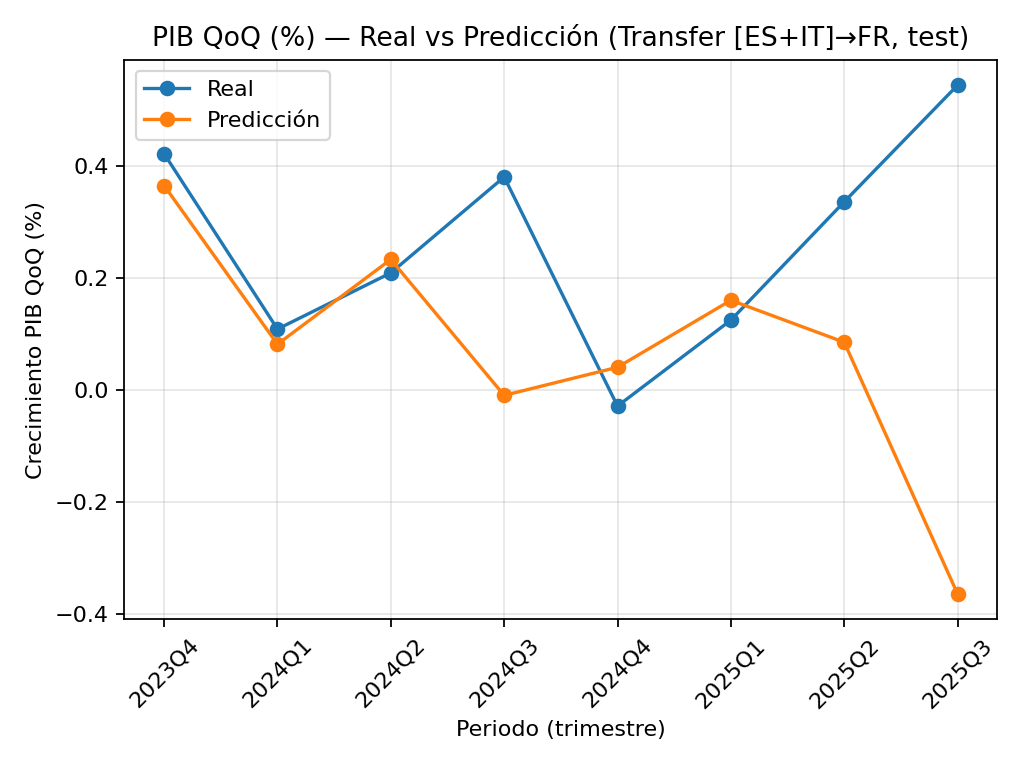
\includegraphics[width=\textwidth]{figures/bloque 3/panel_transfer_ext_fr_real_vs_pred.png}
    \caption{PIB QoQ real vs predicción -- Transfer ES+IT → FR (test)}
    \label{fig:b3_fr_pred}
\end{minipage}\hfill
\begin{minipage}[t]{0.48\textwidth}
    \centering
    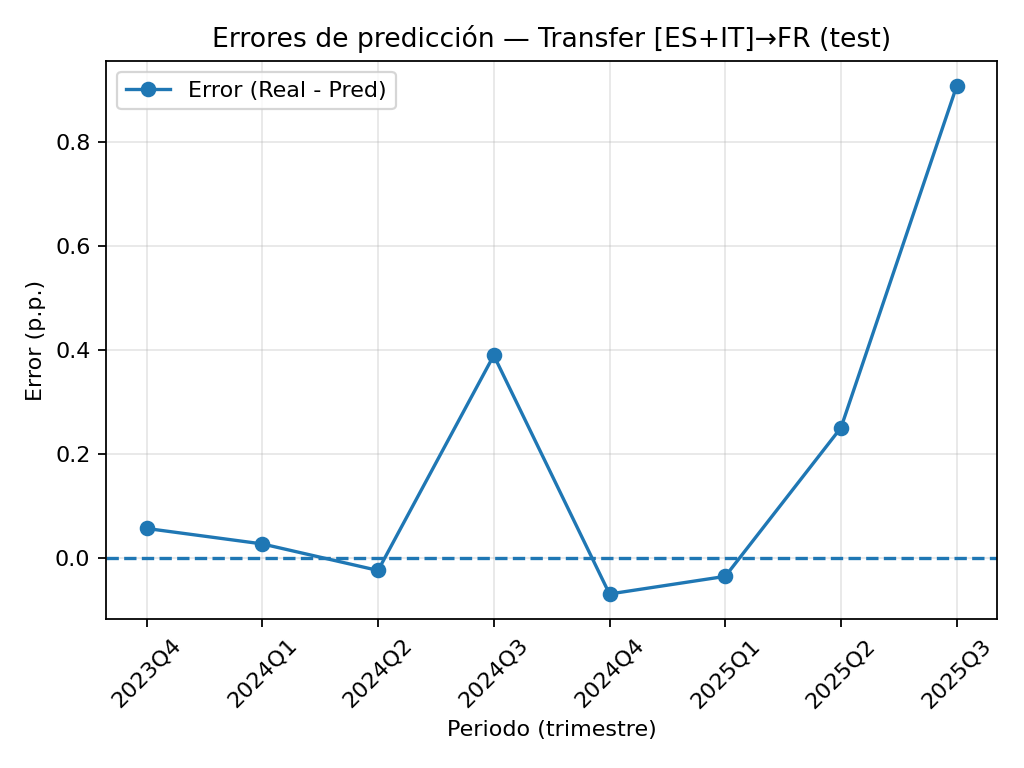
\includegraphics[width=\textwidth]{figures/bloque 3/panel_transfer_ext_fr_errors.png}
    \caption{Errores de predicción -- Transfer ES+IT → FR (test)}
    \label{fig:b3_fr_err}
\end{minipage}
\end{figure}

\FloatBarrier
\subsection{España (FR+IT → ES)}

España obtiene un MAE de 0.337 en transferencia, superior al 0.290--0.297 de los
Bloques~1 y~2, pero muy por debajo del 0.796 que obtenía el modelo ampliado del Bloque~0
con datos españoles propios. La Figura~\ref{fig:b3_es_pred} muestra que el modelo captura
la tendencia general del crecimiento español, aunque con mayor imprecisión que cuando
disponía de datos nacionales en el entrenamiento.

\begin{figure}[H]
\centering
\begin{minipage}[t]{0.48\textwidth}
    \centering
    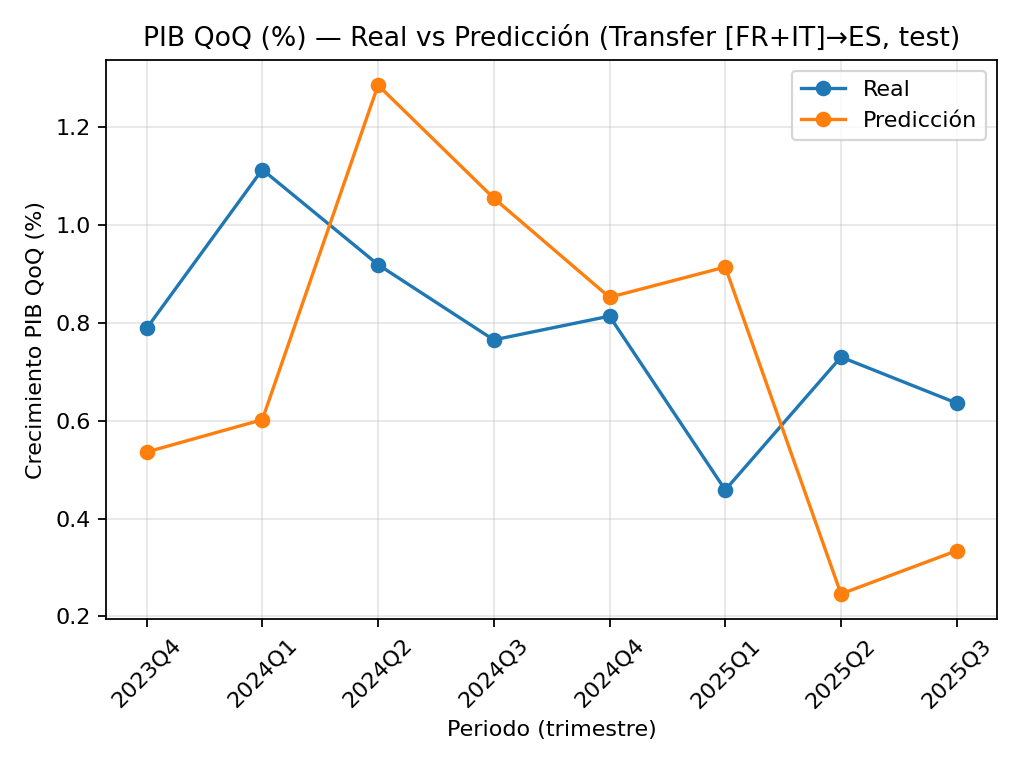
\includegraphics[width=\textwidth]{figures/bloque 3/panel_transfer_ext_es_real_vs_pred.png}
    \caption{PIB QoQ real vs predicción -- Transfer FR+IT → ES (test)}
    \label{fig:b3_es_pred}
\end{minipage}\hfill
\begin{minipage}[t]{0.48\textwidth}
    \centering
    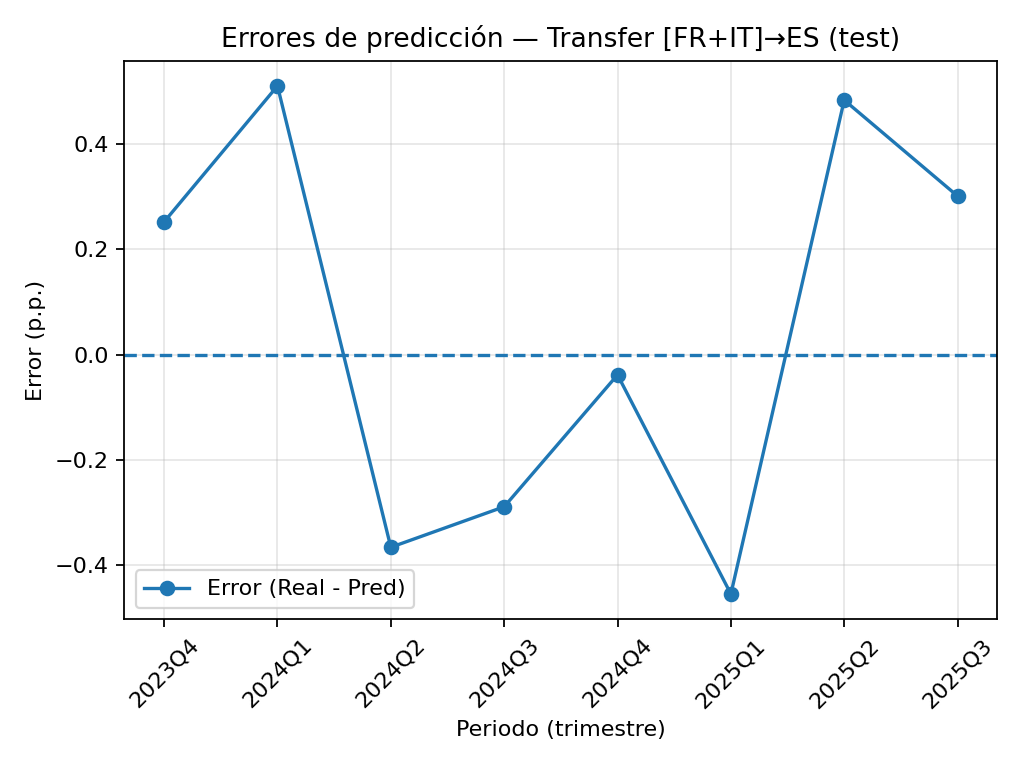
\includegraphics[width=\textwidth]{figures/bloque 3/panel_transfer_ext_es_errors.png}
    \caption{Errores de predicción -- Transfer FR+IT → ES (test)}
    \label{fig:b3_es_err}
\end{minipage}
\end{figure}

\FloatBarrier
\subsection{Síntesis del Bloque 3}

Los resultados del Bloque~3 apuntan a que los patrones macroeconómicos del ciclo
trimestral presentan un grado de transferibilidad entre estas tres economías europeas
mayor del que cabría esperar a priori. En los tres experimentos el modelo obtiene errores
competitivos sin haber visto ningún dato del país de evaluación durante el entrenamiento.

El hallazgo más destacado es el de Italia: el modelo entrenado con ES+FR parece generalizar
mejor a Italia que los modelos entrenados con datos italianos propios en los Bloques~0,
1 y~2. Esto sugiere que la limitada cantidad de observaciones italianas disponibles
introduce más ruido que señal en los bloques donde Italia participa en el entrenamiento,
y que los patrones de España y Francia capturan regularidades cíclicas compartidas que
resultan útiles para estimar el crecimiento italiano.

Para Francia y España, la transferencia produce resultados ligeramente inferiores a los
de los bloques con datos propios (Bloques~1 y~2), lo que es coherente con lo esperado:
la información del propio país durante el entrenamiento aporta valor, pero su ausencia
no impide que el modelo mantenga una capacidad predictiva razonable.

En conjunto, estos resultados apuntan a que los lags del PIB y los indicadores de
actividad económica codifican regularidades del ciclo macroeconómico que son
parcialmente compartidas entre estas economías, lo que podría tener implicaciones
prácticas en contextos donde los datos históricos de un país son escasos o de baja
calidad.		% Plantilla: Se muestran listados
\chapter{Aplicación web de visualización}
\label{app}

\section{Objetivo de la aplicación}

Con el fin de facilitar el análisis e interpretación de los resultados obtenidos en los experimentos, se ha desarrollado una aplicación web interactiva que permite visualizar de forma dinámica las predicciones generadas por los modelos.

La aplicación no realiza entrenamiento en tiempo real, sino que consume los archivos generados automáticamente por el pipeline de modelado (ficheros CSV ubicados en el directorio \texttt{reports/}). De este modo, se mantiene una clara separación entre la fase de entrenamiento y la fase de visualización.

Esta arquitectura garantiza reproducibilidad, modularidad y simplicidad en el mantenimiento del sistema.

\section{Arquitectura del sistema}

La aplicación se integra como la capa final del flujo de trabajo desarrollado a lo largo del proyecto. La arquitectura general puede resumirse de la siguiente manera:

\begin{enumerate}
    \item Descarga de datos mediante la API de Eurostat.
    \item Transformación y cálculo de tasas de variación trimestral.
    \item Construcción del dataset unificado con retardos.
    \item Entrenamiento de modelos predictivos.
    \item Generación de métricas y predicciones en formato CSV.
    \item Visualización interactiva mediante la aplicación web.
\end{enumerate}

Esta estructura modular permite escalar el análisis a nuevos países o modelos sin modificar la lógica de la aplicación.

\section{Interfaz y funcionalidades}

La barra lateral de la aplicación expone tres selectores encadenados que determinan
completamente la vista mostrada:

\begin{itemize}
    \item \textbf{Bloque experimental}: permite elegir entre los tres bloques de
          experimentos implementados --- Bloque~0 (modelos por país), Bloque~1 (panel
          combinado) y Bloque~2 (panel con variable \emph{geo} como feature). La selección
          determina qué conjunto de ficheros CSV se carga.
    \item \textbf{País}: España (ES), Francia (FR) o Italia (IT). Filtra tanto las
          predicciones como las métricas al país seleccionado.
    \item \textbf{Modelo}: configuración base o ampliada. El nombre de la opción se
          adapta al bloque activo (p.ej. ``XGBoost base'' en el Bloque~0,
          ``Panel combinado ampliado'' en el Bloque~1).
\end{itemize}

A partir de estos tres selectores, la aplicación construye dinámicamente las rutas a los
ficheros CSV correspondientes, siguiendo la convención de nombres recogida en la
Tabla~\ref{tab:app_csvs}.

\begin{table}[H]
\centering
\caption{Ficheros CSV leídos por la aplicación según el bloque activo}
\label{tab:app_csvs}
\small
\begin{tabular}{lll}
\hline
\textbf{Bloque} & \textbf{Predicciones} & \textbf{Métricas} \\
\hline
0 & \texttt{predictions\_xgboost\_\{base|ext\}\_\{geo\}.csv}       & \texttt{metrics\_xgboost\_\{geo\}\_compare.csv} \\
1 & \texttt{predictions\_panel\_combined\_\{base|ext\}\_\{geo\}.csv} & \texttt{metrics\_panel\_combined\_compare.csv}  \\
2 & \texttt{predictions\_panel\_geo\_\{base|ext\}\_\{geo\}.csv}      & \texttt{metrics\_panel\_geo\_compare.csv}       \\
\hline
\end{tabular}
\end{table}

En los Bloques~1 y~2 el fichero de métricas contiene los resultados de los tres países en
un único CSV (columna \texttt{geo}); la aplicación filtra automáticamente las filas
correspondientes al país seleccionado. En el Bloque~0 cada país tiene su propio fichero
de métricas.

Una vez cargados los datos, el área principal muestra:

\begin{itemize}
    \item \textbf{Indicadores KPI}: modelo activo, MAE y RMSE en puntos porcentuales,
          y número de variables del modelo.
    \item \textbf{Gráfica de predicción}: comparación entre el PIB QoQ real y el
          predicho a lo largo del conjunto de prueba, generada con Plotly y con
          interactividad nativa (zoom, hover por trimestre).
    \item \textbf{Gráfica de errores}: evolución del error de predicción trimestre a
          trimestre con línea de referencia en cero.
    \item \textbf{Tablas opcionales}: predicciones completas y métricas comparativas,
          activables mediante checkbox en la barra lateral.
\end{itemize}

\section{Decisiones técnicas}

La aplicación ha sido desarrollada con Streamlit, seleccionado por su integración
directa con el ecosistema Python del proyecto y su capacidad para construir interfaces
interactivas sin necesidad de código JavaScript o HTML adicional.

Las visualizaciones se implementan con Plotly, que proporciona interactividad nativa
(zoom, selección de rango, inspección de valores por trimestre) sin coste de desarrollo
adicional respecto a bibliotecas estáticas como Matplotlib.

Se ha optado por una arquitectura desacoplada en la que la aplicación únicamente lee
los CSV generados por los scripts de entrenamiento. Esta separación tiene dos ventajas
concretas: permite actualizar los resultados simplemente re-ejecutando el script de
entrenamiento correspondiente sin tocar la aplicación, y facilita la incorporación de
nuevos bloques experimentales añadiendo únicamente los CSV con la convención de nombres
establecida.

%%%%%%%%%%%%%%%%%%%%%%%%%%%%%%%%%%%%%%%%%%%%%%%%%%%%%%%%%%%%%%%%%%%%%%%%
% Plantilla TFG/TFM
% Escuela Politécnica Superior de la Universidad de Alicante
% Realizado por: Jose Manuel Requena Plens
% Contacto: info@jmrplens.com / Telegram:@jmrplens
%%%%%%%%%%%%%%%%%%%%%%%%%%%%%%%%%%%%%%%%%%%%%%%%%%%%%%%%%%%%%%%%%%%%%%%%

\chapter{Conclusiones}
\label{conclusiones}

Este trabajo ha explorado la aplicación de modelos de aprendizaje automático a la
estimación del crecimiento trimestral del PIB en tres economías de la zona euro ---España,
Francia e Italia--- a través de un diseño experimental progresivo organizado en cuatro
bloques. A lo largo del proyecto se han construido los datos, entrenado y evaluado los
modelos, y desarrollado una herramienta de visualización interactiva que permite explorar
los resultados obtenidos. En esta sección se evalúa el grado de cumplimiento de los
objetivos planteados, se recogen las conclusiones técnicas principales y se señalan las
limitaciones del trabajo y posibles líneas de continuación.

% ══════════════════════════════════════════════════════════════════════
\section{Cumplimiento de objetivos}

\textbf{O1 — Construir un pipeline de datos reproducible.} Se ha implementado un proceso
completo y automatizado de descarga, transformación y estructuración de datos
macroeconómicos procedentes de la API de Eurostat para España, Francia e Italia. El
pipeline cubre desde la obtención de los datos brutos hasta la generación del dataset
panel unificado (\texttt{dataset\_panel\_v1.parquet}), que actúa como fuente única para
todos los experimentos. La modularidad del diseño permite incorporar nuevos países o
indicadores sin modificar la lógica existente. Este objetivo se considera cumplido.

\textbf{O2 — Evaluar la capacidad predictiva de modelos de aprendizaje automático.} Se
han comparado dos configuraciones de XGBoost ---base y ampliada--- bajo cuatro estrategias
de entrenamiento distintas. Los resultados apuntan a que XGBoost supera de forma
consistente a los modelos de regresión lineal de referencia en la mayor parte de los
escenarios analizados, siendo el modelo ampliado (con lags del PIB e indicadores de
actividad) el que mejor rendimiento ofrece cuando dispone de suficiente volumen de datos.
Este objetivo se considera cumplido, con la salvedad de que el reducido tamaño del
conjunto de prueba (8 trimestres) limita la solidez estadística de las comparaciones.

\textbf{O3 — Analizar el efecto del enfoque multi-país.} El diseño experimental ha
permitido explorar tres dimensiones del enfoque multi-país: el entrenamiento conjunto sin
distinción de origen (Bloque~1), la incorporación explícita de la variable de país como
feature (Bloque~2) y la transferencia completa entre economías (Bloque~3). Los resultados
sugieren que combinar datos de varios países puede reducir el sobreajuste cuando las
observaciones individuales por país son escasas, y que los patrones macroeconómicos
presentan un grado de transferibilidad entre estas economías mayor del esperado. Este
objetivo se considera cumplido.

\textbf{O4 — Desarrollar una herramienta de visualización interactiva.} Se ha construido
una aplicación web con Streamlit que permite explorar y comparar los resultados de los
cuatro bloques experimentales para los tres países y las distintas configuraciones de
modelo. La aplicación consume directamente los ficheros CSV generados por el pipeline de
entrenamiento, lo que garantiza la consistencia entre los resultados presentados y los
experimentos realizados. Este objetivo se considera cumplido.

% ══════════════════════════════════════════════════════════════════════
\section{Conclusiones técnicas}

Del conjunto de experimentos realizados se derivan las siguientes conclusiones técnicas
principales:

\textbf{Los lags del PIB son la feature más informativa.} En todos los bloques donde
el modelo ampliado tiene acceso a los retardos del propio PIB
(\texttt{gdp\_qoq\_pct\_l1} y \texttt{gdp\_qoq\_pct\_l2}), estos concentran la mayor
parte de la importancia explicativa según el criterio de ganancia de XGBoost. El
indicador de producción industrial y el comercio minorista rezagados contribuyen de forma
secundaria, mientras que el desempleo y la inflación rezagados presentan una contribución
marginal. Esto sugiere que el nivel reciente de actividad económica es el predictor más
útil del crecimiento trimestral a un horizonte de un trimestre.

\textbf{El enfoque panel parece reducir el sobreajuste.} El caso más ilustrativo es el
del modelo ampliado para España: en el Bloque~0, entrenado solo con datos españoles,
obtenía un MAE de 0.796 debido a una predicción anómala en el primer trimestre del
periodo de prueba; en el Bloque~1, entrenado con los datos de los tres países, el mismo
modelo ampliado obtiene un MAE de 0.297. Este resultado apunta a que el volumen reducido
de observaciones por país es una fuente de sobreajuste relevante en este tipo de
problemas.

\textbf{Las variables de identidad geográfica son secundarias respecto a las
autorregresivas.} El Bloque~2 mostró que añadir dummies de país al modelo ampliado no
aporta mejoras apreciables, ya que el modelo prácticamente ignora esa información cuando
dispone de los lags del PIB. En cambio, cuando el modelo base carece de variables
autorregresivas, las dummies se sobreexplotan y degradan gravemente las predicciones ---con
un MAE de 4.324 en Italia en el peor caso---. Esto sugiere que la identidad del país ya
queda codificada de forma implícita en la dinámica autorregresiva de cada economía.

\textbf{Los patrones del ciclo trimestral parecen ser parcialmente transferibles.} El
Bloque~3 evidenció que es posible obtener predicciones competitivas sobre un país no
visto durante el entrenamiento. El resultado más llamativo fue Italia, cuyo MAE en
transferencia (0.311, entrenando con ES+FR) resultó inferior al de todos los bloques
anteriores en los que Italia sí participaba en el entrenamiento. Este hallazgo apunta a
que los datos de un único país pueden ser insuficientes para aprender sus propios patrones,
y que las regularidades del ciclo macroeconómico compartidas entre economías similares
pueden ser más informativas.

% ══════════════════════════════════════════════════════════════════════
\section{Limitaciones}

Los resultados obtenidos deben interpretarse teniendo en cuenta las siguientes
limitaciones:

\begin{itemize}
    \item \textbf{Tamaño del conjunto de prueba.} El periodo de evaluación comprende
    únicamente 8 trimestres por país. Con un número tan reducido de observaciones, las
    métricas son sensibles a uno o dos errores puntuales y las diferencias entre modelos
    no pueden considerarse estadísticamente significativas.

    \item \textbf{Número de países.} El análisis se limita a tres economías de la zona
    euro. No es posible generalizar las conclusiones sobre transferibilidad o efecto panel
    a otros contextos geográficos o económicos sin experimentos adicionales.

    \item \textbf{Horizonte de predicción.} Todos los modelos estiman el crecimiento del
    trimestre inmediatamente siguiente. No se ha explorado la capacidad de predicción a
    horizontes de dos o más trimestres, donde la degradación del rendimiento previsiblemente
    sería mayor.

    \item \textbf{Variedad de algoritmos.} Los experimentos se centran en XGBoost y
    regresión lineal como referencia. No se han evaluado otros enfoques como Random Forest,
    redes neuronales recurrentes (LSTM) o modelos de series temporales clásicos (ARIMA,
    VAR), lo que impide valorar si las conclusiones son específicas del algoritmo utilizado.

    \item \textbf{Ajuste de hiperparámetros.} Se ha utilizado una configuración fija de
    hiperparámetros para todos los bloques y países. Un proceso de búsqueda sistemática
    podría mejorar los resultados individuales y afectar a las comparaciones entre bloques.
\end{itemize}

% ══════════════════════════════════════════════════════════════════════
\section{Trabajo futuro}

A partir de los resultados y limitaciones identificadas, se proponen las siguientes líneas
de trabajo futuro:

\begin{itemize}
    \item \textbf{Ampliar el panel de países.} Incorporar más economías de la zona euro
    permitiría comprobar si la transferibilidad observada se mantiene con estructuras
    económicas más heterogéneas y aumentaría el volumen de datos disponibles para el
    entrenamiento.

    \item \textbf{Explorar horizontes multi-paso.} Extender los experimentos a predicciones
    de dos o tres trimestres adelante permitiría evaluar la capacidad de los modelos para
    anticipar cambios de tendencia con mayor antelación.

    \item \textbf{Incorporar indicadores adicionales.} Variables como el tipo de interés
    de referencia del BCE, los índices de confianza empresarial o los precios de materias
    primas podrían aportar señal predictiva adicional, especialmente en periodos de cambios
    de política monetaria.

    \item \textbf{Comparar con otros algoritmos.} Evaluar modelos como Random Forest,
    redes LSTM o modelos VAR permitiría determinar si las conclusiones obtenidas son
    específicas de XGBoost o reflejan propiedades más generales del problema.

    \item \textbf{Validación estadística de las comparaciones.} Aplicar tests de
    significación estadística para la comparación de errores de predicción (como el test
    de Diebold-Mariano) permitiría determinar si las diferencias observadas entre modelos
    son estadísticamente relevantes o atribuibles a variabilidad muestral.
\end{itemize}
	% Plantilla: Se muestran matemáticas

%%%%
% CONTENIDO. BIBLIOGRAFÍA.
%%%%
\nocite{*} %incluye TODOS los documentos de la base de datos bibliográfica sean o no citados en el texto
\bibliography{bibliografia/bibliografia} % Archivo que contiene la bibliografía
\bibliographystyle{apacite}

\end{document}
